\section{Motivation}

CASTEP is a leading academic and commercial software package which uses density functional theory to calculate the electronic properties of materials from first principles. One of CASTEP's unique selling points is its ease-of-use for scientists who are not experts in electronic structure theory or numerical methods, that is mainly achieved by intelligent automatic selection of default values for many of the convergence parameters as well as allowing for the selection of precision of most aspects of a calculation from a short list of discrete levels (from \texttt{COARSE} to \texttt{EXTREME}).

Despite this, there is no such intelligent selection available for setting the density of the fine FFT grid used for the on-the-fly (OTF) generation of pseudopotentials, and CASTEP currently defaults to a fine grid size identical to the standard grid used for calculating the Kohn-Sham orbitals. However, this default setting is inadequate for the default OTF pseudopotentials describing a majority of the elements in the periodic table, which require a much finer grid to represent an atom's pseudized core and ultrasoft augmentation charge densities. Additionally, the fine grid density is one of the most difficult parameters to test for convergence due to its strong correlation with plane-wave cutoff, and as a result, many CASTEP calculations are either under-converged (compromising accuracy) or over-converged (wasting CPU time).

This project aimed to remedy this shortcoming by developing and testing scripts for determining a set of \texttt{FINE\_GMAX} values corresponding to \texttt{FINE\_GRID\_SIZE} precision levels from COARSE to EXTREME for a number of supported elements. This database of FINE\_GMAX values would be generated for the C19, QC5 and NCP19 pseudopotential libraries and will be implemented into CASTEP using a lookup table.

The code that has been developed is described in detail in the following section, including a discussion of any prerequisites, troubleshooting, customisation and frequent use-cases.

\section{testgrids.py}

\code{testgrids.py} is a Python 3 script for investigating the behaviour of CASTEP simulations with a varying FINE\_GRID\_SIZE parameter for all supported elements. The script takes care of generating test data, submitting it to the SLURM Workload Manager (SLURM), monitoring the SLURM queue, extracting and plotting the relevant data, as well as saving all relevant data to both machine- and human-readable files.

When running the script with no arguments (\code{python testgrids.py}), the default values for all possible arguments are assumed. The execution begins by checking if a temporary data folder from a previous run with the same name exists; this is \code{tmp} by default, but can be changed with the \code{--name} argument. If this folder exists, it is emptied to prepare it for the data that will be generated during this run. Additionally, a script that deletes any unused semaphores is executed prior to any work being submitted to SLURM.

Next, the job data necessary for this run is generated. By default, a total of 4473 folders is created: 9 different fine grid size values between 2.0 and 6.0, each with 7 different volumes between 94\% and 106\% (as specified by the $\Delta$-project \cite{delta}), for all 71 supported elements that will be simulated. Each folder, named with the corresponding element symbol and a numerical suffix, will contain one \code{.cell} file that details the geometry and parameters of the cell being simulated, and one \code{.param} file that will contain all of the control parameters required to run a CASTEP job. The parent data folder will also contains one \code{.job} file per element, which contains the necessary information for SLURM to treat all jobs corresponding to that element as a single job array and submit it to the queue.

Following the preparation of job data, the script then submits each element as a job array to the SLURM queue, 10 elements at a time by default as to not pollute the queue with too many jobs. At this stage, the progress of job execution is monitored by polling the SLURM queue (every second by default) and reported to the user.

After the completion of all job arrays, the useful data generated by CASTEP needs to be collected and analysed; the reported cell volume and stress, final converged energy, number of iterations that were required for its convergence, total simulation time, fine grid dimensions and real lattice vectors are collected from the new \code{.castep} files and stored in an array. Any warnings or errors during this stage are also reported. The collected volumes and energies are sent to a Birch-Murnaghan equation-of-state (EOS) fitting function that returns the reference volume, bulk modulus and its derivative w.r.t. pressure. On occasions that a good fit cannot be found for any group of volumes, the user is warned and any data for that group is discarded. For all successful fits, $\Delta$-values \cite{delta} are calculated from the EOS data by reference to the EOS data for the largest tested fine grid size of that element. At the end of this stage of execution, all collected values are saved in a human-readable file \code{tmp.table.txt}, all $\Delta$-values are summarised in a machine-readable file \code{tmp.deltas.txt} and the array of collected values is also pickled for further use in \code{tmp.pickle}.

Finally, a 2 by 2 grid of plots is drawn for every element and either shown on screen or saved to a \code{.png} file. The plots show the coarse and fine view of the relationship between the calculated $\Delta$-values and the \code{FINE\_GRID\_SIZE} or corresponding \code{FINE\_GMAX} parameters. When this is completed, the semaphore cleaning script that was used at the beginning of the execution of this script is sent to SLURM again in order to clean up after any potential failures or crashes. If requested (no by default), the \code{tmp} data directory is also deleted, as all useful data has already been saved elsewhere.

\begin{figure}[h]
    \centering
    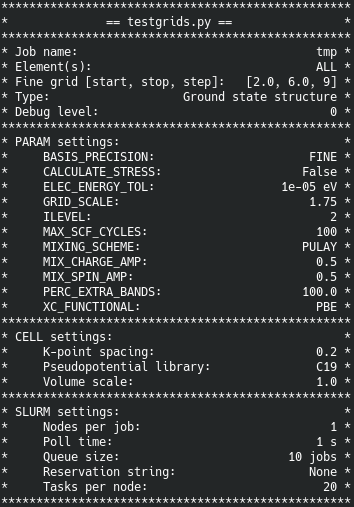
\includegraphics{testgrids_default.png}
    \caption{Summary of all the customisable parameters and their values during a default run. A summary card like this is printed at the beginning of every run, and should be especially useful if the execution output is being logged.}
    \label{fig:testgrids_default}
\end{figure}

\subsection{Installation and Requirements}

The \code{testgrids.py} script does not require any installation or compilation, however, there are a number of mandatory (and optional) packages that are required for the script to work. The list below summarised these requirements, with all quoted version numbers representing the versions that were used during the development and testing of the code. The usage of ``\code{X.X} or higher" here assumes that no changes to the packages will be introduced in the future that will break compatibility with the current requirements. Similarly, it is likely that any package with the same major version will also work, therefore the version numbers in following list can be interpreted as a guidance more than an absolute requirement:

\begin{itemize}
    \item $[$Mandatory$]$ \code{Environment Modules 3.2.10} or higher \cite{modules}
    \item $[$Mandatory$]$ \code{CASTEP 18.1.2} or higher \cite{castep}
    \item $[$Mandatory$]$ \code{Python 3.6.4} or higher \cite{python}
    \item $[$Mandatory$]$ \code{NumPy 1.14.0} or higher \cite{numpy}
    \item $[$Mandatory$]$ \code{Matplotlib 2.1.2} or higher \cite{matplotlib}
    \item $[$Mandatory$]$ any of the following Matplotlib non-interactive backends: \code{agg}, \code{cairo}, \code{gdk}, \code{pdf}, \code{pgf}, \code{ps}, \code{svg}
    \item $[$Optional$]$ any of the following Matplotlib interactive backends: \code{GTK}, \code{GTKAgg}, \code{GTKCairo}, \code{MacOSX}, \code{Qt4Agg}, \code{Qt5Agg}, \code{TkAgg}, \code{WX}, \code{WXAgg}, \code{GTK3Cairo}, \code{GTK3Agg}, \code{WebAgg}, \code{nbAgg}
\end{itemize}

It should be noted that with proper usage of the Environment Modules package, some of the requirements will have to be loaded using the \code{module load} statement before they can be used. On the system where the script was tested, only Python and Matplotlib needed to be loaded, as the script itself takes care of loading CASTEP, and NumPy as well as the required Matplotlib backends were available with Python. If Matplotlib is available as a module separate from Python, as was the case with this system, loading the Matplotlib module will also load the required Python module as a dependency, and therefore the loading of all required modules can be accomplished with a single statement. It should be also be noted that, if the user encounters a syntax error during the execution of the script, this means that Python 2 has been loaded instead of the required Python 3.

Below is also a directory tree showing all the auxiliary files that are included with \code{testgrids.py} along with a short description of their purpose. In order for the script to be able to access these files, its working directory has to be set to its root folder. Files and directories marked with \code{*} are obtained from the $\Delta$ calculation package directly (without any modifications) \cite{delta}, while those marked with \code{**} are also obtained from the same package but have been modified for use with this script.

\hspace{10mm}

\begin{forest}
  for tree={
    font=\ttfamily,
    grow'=0,
    child anchor=west,
    parent anchor=south,
    anchor=west,
    calign=first,
    edge path={
      \noexpand\path [draw, \forestoption{edge}]
      (!u.south west) +(7.5pt,0) |- node[fill,inner sep=1.25pt] {} (.child anchor)\forestoption{edge label};
    },
    before typesetting nodes={
      if n=1
        {insert before={[,phantom]}}
        {}
    },
    fit=band,
    before computing xy={l=15pt},
  }
[\code{testgrids/} \hspace{13.8mm} \small{$\textrm{(root directory)}$}
  [\code{* CIFs/} \hspace{14mm} \small{$\textrm{(directory with CIF files of 71 elemental crystals in their ground state structure)}$}
    [\code{* Ag.cif}]
    [...]
    [\code{* Zr.cif}]
  ]
  [\code{* primCIFs/} \hspace{6.6mm} \small{$\textrm{(directory with CIF files of 71 elemental crystals in a primitive unit cell)}$}
    [\code{* Ag.cif}]
    [...]
    [\code{* Zr.cif}]
  ]
  [\code{* calcDelta.py} \hspace{1mm} \small{$\textrm{(Python script that calculates the } \Delta\textrm{-factor between two data sets)}$}
  ]
  [\code{** eosfit.py} \hspace{4.6mm} \small{$\textrm{(Python script that fits a single set of E(V) data to the Birch-Murnaghan EOS)}$}
  ]
  [\code{ipcclean} \hspace{12mm} \small{$\textrm{(shell script that cleans up unused semaphores from previous SLRUM jobs)}$}
  ]
  [\code{template.job} \hspace{4.6mm} \small{$\textrm{(template shell script for submitting job arrays to SLURM)}$}
  ]
  [\code{testgrids.py} \hspace{4.6mm} \small{$\textrm{(main Python script)}$}
  ]
]
\end{forest}

\subsection{Usage examples}

This section provides examples of common use case scenarios of \code{testgrids.py}, ranging from the most basic (that require only passing a few arguments) to fairly advanced (that may require some editing of code). A full list of all supported arguments, their accepted values and any other relevant information about them is given in a table at the end of this section. Depending on the argument, some text and values have been obtained from the CASTEP \cite{castep_doc} or SLURM \cite{slurm_doc} documentation pages.

\vspace{0.75cm} \noindent
\begin{tabular}{ m{2.5cm} m{13.2cm} }
    \hline \hline
    \textbf{QUESTION}: & I want to do a default run and save the results with the name ``default". I don't care about any temporary files, these can be deleted. \\
    \hline
    \textbf{SOLUTION}: & \code{python testgrids.py --name default --clean true} \\  
    \hline
    \textbf{CONCISE}: & \code{python testgrids.py -na default -cl y} \\   
    \hline
    \textbf{NOTE:} & It is always a good idea to give your run a name, as this is the name that will also be given to all relevant files and plots. \\
    \hline \hline
\end{tabular} 

\vspace{0.75cm} \noindent
\begin{tabular}{ m{2.5cm} m{13.2cm} }
    \hline \hline 
    \textbf{QUESTION}: & I want to do a default run but only for silicon. I also want to open the generated plot in interactive view. \\
    \hline 
    \textbf{SOLUTION}: & \code{python testgrids.py --element Si --save false} \\  
    \hline 
    \textbf{CONCISE}: & \code{python testgrids.py -el Si -sa n} \\
    \hline 
    \textbf{NOTE:} & Using \code{--save false} is not recommended for when a run involves more than a few elements. Interactive plotting windows are opened sequentially (next window opens after the previous one is closed). For all 71 elements, this would represent 71 separate plots. \\
    \hline \hline 
\end{tabular}

\vspace{0.75cm} \noindent
\begin{tabular}{ m{2.5cm} m{13.2cm} }
    \hline \hline 
    \textbf{QUESTION}: & I want to do a default run but over a higher range (1.5 to 6.5) and with a larger density (0.1) of \code{FINE\_GRID\_SIZE} values. \\
    \hline 
    \textbf{SOLUTION}: & \code{python testgrids.py --fine\_grid\_min 1.5 --fine\_grid\_max 6.5 ...} \code{... --fine\_grid\_step 51 --name long\_run} \\
    \hline 
    \textbf{CONCISE}: & \code{python testgrids.py -f0 1.5 -f1 6.5 -fs 51 -na long\_run} \\
    \hline 
    \textbf{NOTE:} & A run with 51 \code{FINE\_GRID\_SIZE} steps and the default number of elements will require $51*7*71=25,347$ total jobs, which will take a significant time to complete. When starting a long run, it is recommended to verify that the run behaves and gives results as expected, usually by doing a preliminary run with a single element or a smaller number of steps. \\
    \hline \hline 
\end{tabular} 

\vspace{0.75cm} \noindent
\begin{tabular}{ m{2.5cm} m{13.2cm} }
    \hline \hline 
    \textbf{QUESTION}: & I have a lot of nodes with 64 cores available to me under the reservation ``El\_Psy\_Kongroo". As my run involves large jobs, I want each job to run on 2 nodes. \\
    \hline 
    \textbf{SOLUTION}: & \code{python testgrids.py --reserve El\_Psy\_Kongroo --tasks 64 --nodes 2 ...} \code{... --queue 100} \\
    \hline 
    \textbf{CONCISE}: & \code{python testgrids.py -r El\_Psy\_Kongroo -t 64 -no 2 -q 100} \\
    \hline 
    \textbf{NOTE:} & The semaphore cleanup script is not available when using \code{--reserve}, so any necessary cleanup needs to be done before starting the run. When using \code{--tasks} and \code{--nodes}, it is important to know the number of cores available per node, as well as the performance implications of running a job across many cores and nodes. Setting a large value for \code{--queue} will submit an equally large number of job arrays to the SLURM queue (or all jobs waiting to be submitted, whichever is smaller), therefore it is important to be mindful of this if you aren't using reserved nodes. \\
    \hline \hline 
\end{tabular}

\vspace{0.75cm} \noindent
\begin{tabular}{ m{2.5cm} m{13.2cm} }
    \hline \hline 
    \textbf{QUESTION}: & I am testing the behaviour of a new set of values for some parameters, and would like the script to be as verbose as possible. As I am logging the output, I do need frequent infromation about job progress in the SLURM queue. \\
    \hline 
    \textbf{SOLUTION}: & \code{python testgrids.py --name test --debug 1 --poll\_wait 60 >> test.log} \\
    \hline 
    \textbf{CONCISE}: & \code{python testgrids.py -na test -d 1 -po 60 >> test.log} \\
    \hline 
    \textbf{NOTE:} & Using \code{--debug 1} will enable debugging mode that, at level 1, only enables verbose output. At higher levels, debug mode is used to control the flow of code (this is discussed further in the next section) and should not be used unless you understand the implications of the value you have chosen. Setting \code{--poll\_wait} to higher values increases the time between successive checks of the SLURM queue, that in turn decreases the amount of repetitive output. However, jobs that are pending to be submitted to the queue can only be submitted after the queue reports that it is empty, therefore very high values of \code{--poll\_wait} are likely to waste time by leaving the SLURM queue empty for longer.\\
    \hline \hline 
\end{tabular}

\vspace{0.75cm} \noindent
\begin{tabular}{ m{2.5cm} m{13.2cm} }
    \hline \hline 
    \textbf{QUESTION}: & I have completed a run previously and have the relevant \code{.pickle} file. I would like to open these plots in interactive view again. \\
    \hline 
    \textbf{SOLUTION}: & \code{python testgrids.py --load old\_run.pickle --save false} \\
    \hline 
    \textbf{CONCISE}: & \code{python testgrids.py -l old\_run.pickle -sa n} \\
    \hline 
    \textbf{NOTE:} & When using \code{--load}, the built-in argument parser will ignore all arguments besides \code{--save}. This way, it is possible to either revisit old data using interactive plots, or re-plot old data and save the figures when the previous ones are no longer available or were never plotted. This is especially useful for runs with a reused \code{--name} argument that did not save any new figures (\code{testgrids.py} will not overwrite an existing directory in \code{./figs}). Similar functionality can be achieved by repeating your run with identical arguments and adding \code{--debug 4}, however, the former method is preferred. \\
    \hline \hline 
\end{tabular}

\vspace{0.75cm} \noindent
\begin{tabular}{ m{2.5cm} m{13.2cm} }
    \hline \hline 
    \textbf{QUESTION}: & I would like to do a run involving the calculation of a stress tensor on elemental crystals in their primitive unit cell. \\
    \hline 
    \textbf{SOLUTION}: & \code{python testgrids.py --primitive true --stress true} \\
    \hline 
    \textbf{CONCISE}: & \code{python testgrids.py -pr y -st y} \\
    \hline 
    \textbf{NOTE:} & Choosing to run calculations on elemental crystals in their primitive unit cell instead of the default ground state structure will allow for faster calculations, however, the results will no longer be interpretable in the same way as those quoted on the $\Delta$-project website. Enabling calculations of the stress tensor will also increase the total calculation time. The pressure (in GPa) will be visible in the \code{name.table.txt} file, however, this setting should have no effect on the generated plots. \\
    \hline \hline 
\end{tabular}

\vspace{0.75cm} \noindent
\begin{tabular}{ m{2.5cm} m{13.2cm} }
    \hline \hline 
    \textbf{QUESTION}: & I would like to tweak some arguments relating to the density mixing procedure. \\
    \hline 
    \textbf{SOLUTION}: & \code{python testgrids.py --mix\_scheme broyden --mix\_charge\_amp 0.8 ...} \code{... --mix\_spin\_amp 1.75} \\
    \hline 
    \textbf{CONCISE}: & \code{python testgrids.py -mi broyden -mc 0.8 -ms 1.75} \\
    \hline 
    \textbf{NOTE:} & When experiencing SCF convergence failures, it is often helpful to switch \code{--mix\_scheme} between Pulay and Broyden, as well as decreasing the mixing amplitude for the charge and spin density arguments. \\
    \hline \hline 
\end{tabular}

\vspace{0.75cm} \noindent
\begin{tabular}{ m{2.5cm} m{13.2cm} }
    \hline \hline 
    \textbf{QUESTION}: & I would like to do a run involving a metal or finite-temperature insulator. I would also like to also increase the precision of this run in all available aspects. \\
    \hline 
    \textbf{SOLUTION}: & \code{python testgrids.py --extra\_bands 120 --basis\_prec precise ...} \code{... --elec\_enrg\_tol 1e-8 --grid 2.5 --kpoint\_spacing 0.15 ...} \code{... --max\_scf\_cycles 200} \\
    \hline 
    \textbf{CONCISE}: & \code{python testgrids.py -ba 120 -bp precise -ee 1e-8 -g 2.5 -k 0.15 -sc 200} \\
    \hline 
    \textbf{NOTE:} & When dealing with metals or finite-temperature insulators, it can be useful to increase the number of available bands using \code{--extra\_bands}. Although the default value of \code{--extra\_bands 100} should be enough for most scenarios, no significant performance losses were measured with using higher values. It should be noted that the above combination of parameters does not necessarily correspond to a real-life scenario, and is instead used for demonstration of the available arguments. Good understanding of the advantages and drawbacks of the above parameters and their combinations is essential in obtaining meaningful results from a run. Setting \code{--basis\_prec} to a higher level increases the precision of convergence of atomic energies with respect to the plane wave cutoff energy. Decreasing \code{--elec\_enrg\_tol} decreases the tolerance for accepting convergence of the total energy in an electronic minimisation. Increasing \code{--grid} increases the size of the standard grid, relative to the diameter of the cutoff sphere (it is important to be aware that changes to this argument also impacts \code{FINE\_GRID\_SIZE}, which is defined relative to \code{GRID\_SIZE}). Choosing a smaller \code{--kpoint\_spacing} increases the k-point density in reciprocal space, in turn increasing the smoothness of the ground state energy well. Increasing \code{--max\_scf\_cycles} increases the maximum number of SCF cycles performed in an electronic minimisation, therefore reducing the likelihood of failed convergence (although frequent SCF convergence failures often point to a different problem). A well thought-out combination of some or all of these arguments backed by a number of preliminary runs is often required. It should also be obvious that tweaking most of these parameters will have a noticeable impact on the performance of a run. \\
    \hline \hline 
\end{tabular}

\vspace{0.75cm} \noindent
\begin{tabular}{ m{2.5cm} m{13.2cm} }
    \hline \hline 
    \textbf{QUESTION}: & I would like to use the LDA exchange-correlation functional for this run. Since the LDA description tends to overbind atoms and underestimate cell volume, I would like to apply a +3\% cell volume correction before $\Delta$ calculations take place. \\
    \hline 
    \textbf{SOLUTION}: & \code{python testgrids.py --xc\_functional LDA --volume\_scale 1.03} \\
    \hline 
    \textbf{CONCISE}: & \code{python testgrids.py -x LDA -v 1.03} \\
    \hline 
    \textbf{NOTE:} & Cell volume scaling is applied before any $\Delta$-project relevant calculations take place; the \code{--volume\_scale} argument can therefore be useful if you encounter a lot of fitting errors from the Birch-Murnaghan EOS fitting function. The \code{--xc\_functional} argument currently supports a large number of functionals, including all the functionals documented in CASTEP 18.1. If you know that the CASTEP version you are using includes support for a functional that is not supported by \code{testgrids.py}, you can add it yourself: open \code{testgrids.py} in your preferred editor, scroll down to the \code{parse\_args(...)} function, look for a statement with \code{args.xc\_functional} and a list of functionals, and add your functional to the list. If a functional that is not currently supported becomes popular, I will endeavour to update the list. \\
    \hline \hline 
\end{tabular}

\vspace{0.75cm} \noindent
\begin{tabular}{ m{2.5cm} m{13.2cm} }
    \hline \hline 
    \textbf{QUESTION}: & I would like to use a different version of CASTEP for this run, and because I'm doing some testing, I would like to increase the verbosity of the generated \code{.castep} files. \\
    \hline 
    \textbf{SOLUTION}: & \code{python testgrids.py --castep CASTEP/19.11 --ilevel 3} \\
    \hline 
    \textbf{CONCISE}: & \code{python testgrids.py -ca CASTEP/19.11 -i 3} \\
    \hline 
    \textbf{NOTE:} & Although CASTEP's \code{IPRINT} argument accepts values of 1, 2 and 3, \code{--ilevel} does not support level 1 as this option does not produce a verbose enough output in the \code{.castep} files for scraping the required information. Level 2 is the default, and it can be increased up to level 3 for additional verbosity. If a different CASTEP version is to be used for all runs, it is fairly simple to edit the default CASTEP module used by \code{testgrids.py} to avoid having to use the \code{--castep} argument with every run: open \code{testgrids.py} in your preferred editor, scroll down to the \code{parse\_args(...)} function, look for a statement with \code{args.castep = "CASTEP/19.1.1-foss-2018a"} and edit the string to match the name of your CASTEP module. \\
    \hline \hline 
\end{tabular}

\vspace{0.75cm} \noindent
\begin{tabular}{ m{2.5cm} m{13.2cm} }
    \hline \hline 
    \textbf{QUESTION}: & I have a directory containing \code{.cif} files which I would like to use for my run. \\
    \hline 
    \textbf{SOLUTION}: & \code{python testgrids.py --cif\_dir /path/to/dir}\\
    \hline 
    \textbf{CONCISE}: & \code{python testgrids.py -cf /path/to/dir} \\
    \hline 
    \textbf{NOTE:} & When \code{--cif\_dir} is specified, the \code{--primitive} argument is ignored. This argument is especially useful for doing a run involving a subset of elements from \code{.cif} files already provided with \code{testgrids.py}: simply copy the elements of your choice into a new directory, and supply the path to that directory (either relative or absolute) to the \code{--cif\_dir} argument. When using custom \code{.cif} files, it is essential that the files contain enough information for CASTEP's \code{cif2cell} script to generate a \code{.cell} file containing \code{BLOCK LATTICE\_CART}, \code{BLOCK POSITIONS\_FRAC}, \code{BLOCK SPECIES\_POT} and \code{BLOCK SYMMETRY\_OPS}. \\
    \hline \hline 
\end{tabular}

\vspace{0.75cm} \noindent
\begin{tabular}{ m{2.5cm} m{13.2cm} }
    \hline \hline 
    \textbf{QUESTION}: & I would like to use specific pseudopotential library for my run. \\
    \hline 
    \textbf{SOLUTION}: & \code{python testgrids.py --pseudo\_pot NCP19}\\
    \hline 
    \textbf{CONCISE}: & \code{python testgrids.py -ps NCP19} \\
    \hline 
    \textbf{NOTE:} & The list of possible pseudopotential libraries that can be officially used with \code{testgrids.py} is limited to only C19, QC5 and NCP19. Although this script was not intended for use with other libraries that are available with CASTEP, adding your own pseudopotential to the list of supported ones should not cause any issues: open \code{testgrids.py} in your preferred editor, scroll down to the \code{parse\_args(...)} function, look for a statement with \code{args.pseudo\_pot} and a list of pseudopotential libraries, and add your library to the list. Furthermore, the list of libraries is not necessarily limited to libraries: you may add \code{.otfglib}, \code{.usp}, \code{.uspcc}, \code{.uspso}, \code{.recpot}, \code{.upf}, \code{.dat} or  \code{.data} files (with their file extension), as well as a valid OTFG pseudopotential string to the list. If your usage of \code{testgrids.py} will involve a number unsupported pseudopotentials, you may simply comment out the \code{if} block containing \code{args.pseudo\_pot} to suppress the check carried out by the argument parser. \\
    \hline \hline 
\end{tabular}

\clearpage

\begin{table}[!h]
\centering
\begin{tabularx}{1\linewidth}{|c|c|c|c|>{\hsize=.6\hsize\linewidth=\hsize}Y|>{\hsize=1.4\hsize\linewidth=\hsize}Y|}
\hline
\textbf{Argument} & \textbf{Abbr.} & \textbf{Type} & \textbf{Default} & \textbf{Accepted values} & \textbf{Notes} \\ \hline

\code{--extra\_bands} & \code{-ba} & \code{float} & \code{100.0} & any $\geq 0$ & Controls the percentage of extra bands in addition to the number of occupied bands (necessary for metals or finite temperature insulators). Corresponds to the CASTEP \code{.param} file keyword \code{PERC\_EXTRA\_BANDS}. \\ \hline

\code{--basis\_prec} & \code{-bp} & \code{str} & \code{"FINE"} & any one of \code{COARSE}, \code{MEDIUM}, \code{FINE}, \code{PRECISE} or \code{EXTREME} & Specifies the precision of the basis set by choosing the level of convergence of atomic energies with respect to the plane wave cutoff energy. Corresponds to the CASTEP \code{.param} file keyword \code{BASIS\_PRECISION}. \\ \hline

\code{--castep} & \code{-ca} & \code{str} & \code{""} & any string corresponding to a CASTEP module that can be loaded & Specifies the CASTEP module that will be used during the exacution of the script. Validated by attempting to load the specified module in a clean environment. If no value provided, argument defaults to \code{CASTEP/19.1.1-foss-2018a} \\ \hline

\code{--clean} & \code{-cl} & \code{bool} & \code{False} & any string than can be interpreted as a boolean & Specifies whether the temporary data folder should be deleted at the end of the execution of the script. \\ \hline

\code{--cif\_dir} & \code{-cf} & \code{str} & \code{""} & any string corresponding to a valid path to a directory & Specifies the directory containing the \code{.cif} files to be used. Validated by checking the existence of the directory. If no value provided, argument defaults to either \code{./CIFs} or \code{./primCIFs} depending on the value of the \code{--primitive} argument\\ \hline

\code{--debug} & \code{-d} & \code{int} & \code{0} & any $\geq 0$ & Specifies the debug level, increasing script verbosity and controlling code flow.\\ \hline

\code{--elec\_enrg\_tol} & \code{-ee} & \code{float} & \code{1e-5} & any $> 0$ & Controls the tolerance for accepting convergence of the total energy in an electronic minimisation. Corresponds to the CASTEP \code{.param} file keyword \code{ELEC\_ENERGY\_TOL}. \\ \hline

\code{--element} & \code{-el} & \code{str} & \code{""} & any string corresponding to a symbol of an element present in the CIFs directory & Specifies which single element to simulate, validated by verifying the existence of a corresponding .cif file in the directory specified by \code{--cif\_dir}. If no value provided, argument defaults to all elements in the CIFs folder \\ \hline

\code{--fine\_grid\_min} & \code{-f0} & \code{float} & \code{2.0} & $1 \leq$ any $\leq$ \code{-f1} & Specifies the lowest value of the CASTEP \code{.param} file keyword \code{FINE\_GRID\_SCALE}. \\ \hline

\code{--fine\_grid\_max} & \code{-f1} & \code{float} & \code{6.0} & any $\geq$ \code{-f0} &  Specifies the highest value of the CASTEP \code{.param} file keyword \code{FINE\_GRID\_SCALE}. \\ \hline

\code{--fine\_grid\_step} & \code{-fs} & \code{int} & \code{9} & any $\geq 2$ & Specifies the number of samples between \code{--fine\_grid\_min} and \code{--fine\_grid\_max} (inclusive). \\ \hline

\code{--grid} & \code{-g} & \code{float} & \code{1.75} & any $\geq 1$ & Specifies the fixed value of the CASTEP \code{.param} file keyword \code{GRID\_SCALE}. \\ \hline

\code{--ilevel} & \code{-i} & \code{int} & \code{2} & 2 or 3 & Specifies the level of verbosity of \code{.castep} files. Corresponds to the CASTEP \code{.param} file keyword \code{IPRINT}. \\ \hline

\code{--kpoint\_spacing} & \code{-k} & \code{float} & \code{0.2} & any $> 0$ & Specifies the k-point density of a Monkhorst-Pack grid (units of inverse length). Corresponds to the CASTEP \code{.cell} file keyword \code{KPOINT\_MP\_SPACING}. \\ \hline

\code{--load} & \code{-l} & \code{str} & \code{""} & Any string corresponding to a valid path to a file & Specifies the path to a \code{.pickle} file that will be loaded instead of running any simulations. Validated by verifying the existence of the specified file. \\ \hline

\end{tabularx}
\caption{Summary of optional arguments that can be passed to the \code{testgrids.py} (Part 1: [a-l])}
\label{tab:arguments1}
\end{table}

\clearpage

\begin{table}[!h]
\centering
\begin{tabularx}{1\linewidth}{|c|c|c|c|>{\hsize=.6\hsize\linewidth=\hsize}Y|>{\hsize=1.4\hsize\linewidth=\hsize}Y|}
\hline
\textbf{Argument} & \textbf{Abbr.} & \textbf{Type} & \textbf{Default} & \textbf{Accepted values} & \textbf{Notes} \\ \hline

\code{--mix\_charge\_amp} & \code{-mc} & \code{float} & \code{0.5} & any $> 0$ & Determines the mixing amplitude for the charge density in the density mixing procedure. Corresponds to the CASTEP \code{.param} file keyword \code{MIX\_CHARGE\_AMP}. \\ \hline

\code{--mix\_scheme} & \code{-mi} & \code{str} & \code{"PULAY"} & any one of \code{BROYDEN}, \code{KERKER}, \code{LINEAR} or \code{PULAY} & Determines which mixing scheme will be used in the density mixing procedure. Corresponds to the CASTEP \code{.param} file keyword \code{MIXING\_SCHEME}. \\ \hline

\code{--mix\_spin\_amp} & \code{-ms} & \code{float} & \code{0.5} & any $> 0$ & Determines the mixing amplitude for the spin density in the density mixing procedure. Corresponds to the CASTEP \code{.param} file keyword \code{MIX\_SPIN\_AMP}. \\ \hline

\code{--name} & \code{-na} & \code{str} & \code{"tmp"} & any string & Specifies the name of this run, corresponding to the filenames of the generated files and the temporary simulation data directory. \\ \hline

\code{--nodes} & \code{-no} & \code{int} & \code{1} & any $\geq 1$ & Corresponds to the number of SLURM nodes that will be assigned to each job array. \\ \hline

\code{--poll\_wait} & \code{-po} & \code{int} & \code{1} & any $\geq 1$ & Specifies the time in seconds to wait between polling the SLURM \code{squeue} (used for tracking job progress). Higher values may waste time by not scheduling new jobs in time, while lower values may slow down the machine. \\ \hline

\code{--primitive} & \code{-pr} & \code{bool} & \code{False} & any string that can be interpreted as a boolean & Specifies whether the primitive unit cell .cif files should be used instead of ground-state structure .cif files. Setting to \code{True} will reduce job time but may yield inaccurate results. \\ \hline

\code{--pseudo\_pot} & \code{-ps} & \code{str} & \code{"C19"} & any one of \code{C19}, \code{QC5}, or \code{"NCP19"} & Specifies the pseudopotential library that will be used during this run. Corresponds to the CASTEP \code{.cell} file keyword \code{SPECIES\_POT}. \\ \hline

\code{--queue} & \code{-q} & \code{int} & \code{10} & any $\geq 1$ & Specifies the maximum number of job arrays that will be submitted to the SLURM queue at a time. \\ \hline

\code{--reserve} & \code{-r} & \code{str} & \code{""} & any string & Specifies the reservation string used when submitting a job array to the SLURM queue. \\ \hline

\code{--save} & \code{-sa} & \code{bool} & \code{True} & any string that can be interpreted as a boolean & Specifies whether plots should be saved to \code{.png} files in the \code{./figs} directory, or drawn on screen. \\ \hline

\code{--max\_scf\_cycles} & \code{-sc} & \code{int} & \code{100} & any $\geq 1$ & Determines the maximum number of SCF cycles performed in an electronic minimisation. Corresponds to the CASTEP \code{.param} file keyword \code{MAX\_SCF\_CYCLES}. \\ \hline

\code{--stress} & \code{-st} & \code{bool} & \code{False} & any string that can be interpreted as a boolean & Controls whether or not a stress calculation will be performed. Setting to \code{True} will increase job time. \\ \hline

\code{--tasks} & \code{-t} & \code{int} & 20 & any $\geq 1$ & Specifies the number of SLURM tasks that a single job should use per node. \\ \hline

\code{--volume\_scale} & \code{-v} & \code{float} & \code{1.0} & any $> 0$ & Specifies the cell volume scale factor that will be applied on top of $\Delta$ project-relevant volume adjustments. \\ \hline

\end{tabularx}
\caption{Summary of optional arguments that can be passed to the \code{testgrids.py} (Part 2: [m-v])}
\label{tab:arguments2}
\end{table}

\clearpage

\begin{table}[!h]
\centering
\begin{tabularx}{1\linewidth}{|c|c|c|c|>{\hsize=1.2\hsize\linewidth=\hsize}Y|>{\hsize=0.8\hsize\linewidth=\hsize}Y|}
\hline
\textbf{Argument} & \textbf{Abbr.} & \textbf{Type} & \textbf{Default} & \textbf{Accepted values} & \textbf{Notes} \\ \hline

\code{--xc\_functional} & \code{-x} & \code{str} & \code{"PBE"} & any one of \code{"LDA"}, \code{"PW91"}, \code{"PBE"}, \code{"PBESOL"}, \code{"RPBE"}, \code{"WC"}, \code{"BLYP"}, \code{"LDA-C2"}, \code{"LDA-X"}, \code{"ZERO"}, \code{"HF"}, \code{"PBE0"}, \code{"B3LYP"}, \code{"HSE03"}, \code{"HSE06"}, \code{"EXX-X"}, \code{"HF-LDA"}, \code{"EXX"}, \code{"EXX-LDA"}, \code{"SHF"}, \code{"SX"}, \code{"SHF-LDA"}, \code{"SX-LDA"}, \code{"WDA"}, \code{"SEX"} or \code{"SEX-LDA"} & Controls which functional is used to calculate the exchange-correlation potential. Corresponds to the CASTEP \code{.param} file keyword \code{XC\_FUNCTIONAL}. \\ \hline

\end{tabularx}
\caption{Summary of optional arguments that can be passed to the \code{testgrids.py} (Part 3: [x])}
\label{tab:arguments3}
\end{table}

\subsection{Troubleshooting}

Although care has been taken to select a set of default parameters that minimise the rate of errors that can occur during the execution of the code, some errors with specific combinations of elements and corresponding parameters still remain. This section summarises all the possible ways in which code can fail; this includes non-critical errors (runtime errors in the SLURM queue, CASTEP jobs or EOS fitting function) as well as critical errors (often missing modules, permission issues, missing files, misspelled paths, or low disk space), and how to remedy them.

\begin{table}[h]
\begin{tabularx}{1\linewidth}{|>{\hsize=0.6\hsize\linewidth=\hsize}Y|c|>{\hsize=1.4\hsize\linewidth=\hsize}Y|}
\hline \hline
\textbf{Error message} & \textbf{Level} & \textbf{Notes} \\ \hline
\code{[WARNING] found .err file} \code{in dir ...} & NCE & This non-critical error is reported when the presence of an \code{.err} file is detected in any temporary job directory. The file is created by CASTEP when it encounters a runtime error such as a convergence failure or a non-variational total energy, and the contents of file should provide enough information regarding the error and how to remedy it. The presence of this error also means that a $\Delta$ value will not be calculated for that corresponding \code{FINE\_GRID\_SIZE} value of the element. \\ \hline
\code{[WARNING] job ... has} \code{encountered an error or} \code{been killed} & NCE & This non-critical error is reported when the presence the words ``error" or ``killed" is detected in an \code{.out} file. The error is reported by SLURM when a job exits with a non-zero return code (it failed in some way), or if the job has been killed (it requested more memory than is available, or exceeded the maximum allocated time); the contents of the file usually provides enough information regarding this error. The presence of this error also means that a $\Delta$ value will not be calculated for that corresponding \code{FINE\_GRID\_SIZE} value of the element. \\ \hline
\code{[WARNING] over 5 warnings} \code{detected in file ...} & W & This warning is reported when more than 5 occurrences of the word ``warning" are detected in the \code{.castep} file. Although some warnings during the first few steps of convergence are common, a large number of warnings may point to an issue that needs investigating. \\ \hline
\code{[DEBUG] discarded as EOS} \code{fitting function returned} \code{a complex or None type} \code{(not float)} & NCE & This non-critical error is reported when the Birch-Murnaghan EOS fitting function returns a complex number or \code{None} as a value for at least one EOS parameter. The error is a result of an inadequate or failed fit; inspecting the \code{name.table.txt} file to deduce whether the relevant E-V curve has a minimum, and adjusting parameters such as \code{--volume\_scale}, \code{--kpoint\_spacing}, \code{--elec\_enrg\_tol} or \code{--basis\_prec} should remedy this. The presence of this error also means that a $\Delta$ value will not be calculated for that corresponding \code{FINE\_GRID\_SIZE} value of the element. \\ \hline
\code{[DEBUG] discarded as EOS} \code{fitting function returned} \code{a negative bulk modulus} \code{derivative} & NCE & This non-critical error is simmilar to the previous one: it results from an inadequate fit, can be remedied in the same ways as the previous error, and also results in a $\Delta$ value being omitted. The difference between them is that this error is triggered when the EOS fitting function returns a negative bulk modulus derivative - an unphysical result.  \\ \hline \hline
\end{tabularx}
\caption{Summary of all possible non-critical errors and warnings, presented in order of the execution stage during which they can occur; [NCE] = Non-critical error, [W] = Warning}
\label{tab:troubleshooting1}
\end{table}

\begin{table}[h]
\begin{tabularx}{1\linewidth}{|c|>{\hsize=1\hsize\linewidth=\hsize}Y|>{\hsize=1\hsize\linewidth=\hsize}Y|}
\hline \hline
\textbf{Return code} & \textbf{Corresponding error} & \textbf{Notes} \\ \hline
\code{00} & None & Execution finished without encountering errors \\ \hline \hline
\code{01} & \code{ImportError} when importing modules & Check all required modules are installed \\ \hline
\code{02} & arg directory does not exist or is inaccessible & Check spelling and permissions of directory \\ \hline
\code{03} & arg file does not exist or is inaccessible & Check spelling and permission of file \\ \hline
\code{04} & \code{TypeError} when parsing args & Check the required arg types in Tables \ref{tab:arguments1}, \ref{tab:arguments2}, \ref{tab:arguments3} \\ \hline
\code{05} & arg out of bounds & Check the arg accepted values in Tables \ref{tab:arguments1}, \ref{tab:arguments2}, \ref{tab:arguments3} \\ \hline
\code{06} & arg not one of possible options & Check the arg accepted values in Tables \ref{tab:arguments1}, \ref{tab:arguments2}, \ref{tab:arguments3} \\ \hline
\code{07} & \code{CalledProcessError} when loading CASTEP & Use \code{--castep} for different CASTEP module \\ \hline \hline
\code{10} & \code{OSError} while generating job data & Check write permissions and remaining space \\ \hline
\code{11} & \code{CalledProcessError} while generating data & Verify that \code{cif2cell} is available in PATH \\ \hline
\code{19} & uncaught exception while generating job data & Inspect error message for more details \\ \hline \hline
\code{20} & \code{CalledProcessError} while running jobs & Verify that \code{sbatch} and \code{squeue} are available \\ \hline
\code{29} & uncaught exception while running jobs & Inspect error message for more details \\ \hline \hline
\code{30} & \code{OSError} while reading job output data & Check \code{testgrids.py} has read permissions \\ \hline
\code{31} & \code{PickleError} when saving array data to disk & Check write permissions and available space \\ \hline
\code{39} & uncaught exception while read job output data & Inspect error message for more details \\ \hline \hline
\code{40} & \code{OSError} while cleaning up & Check write permissions or close opened files \\ \hline
\code{49} & uncaught exception while cleaning up & Inspect error message for more details \\ \hline \hline
\code{50} & \code{OSError} while opening pickle file handle & Check read permissions and path spelling \\ \hline
\code{51} & \code{PickleError} when loading pickle data & Verify pickle file is valid and not corrupted \\ \hline
\code{59} & uncaught exception while loading data arrays & Inspect error message for more details \\ \hline \hline
\code{69} & uncaught exception while deleting semaphores & Inspect error message for more details \\ \hline \hline
\end{tabularx}
\caption{Summary of all possible critical errors. As all of these errors cease the execution of the script, the corresponding return codes are also provided.}
\label{tab:troubleshooting2}
\end{table}

When debugging, it is possible to use the \code{--debug} flag to skip to a various execution points of the code. This is useful when an uncaught exception occurs in a part of the code; when adequate changes are made, the code execution can resume at around that point (assuming all prerequisites for code execution at that point are met). If ``resuming'' code execution this way, the same parameters must be used as those that were used previously, and for which runtime-related files have already been created. The table below gives a full list of allowed \code{--debug} values:

\begin{table}[h]
\begin{tabularx}{1\linewidth}{|c|>{\hsize=1\hsize\linewidth=\hsize}Y|}
\hline
\textbf{Debug level} & \textbf{Notes} \\ \hline
0 (default) & Code runs from beginning to end with minimal verbosity \\ \hline
1 & Code runs from beginning to end with increased verbosity \\ \hline
2 & Code skips initial cleaning of semaphores and cleaning of working directory; execution starts at generation of job data \\ \hline
3 & Code skips everything mentioned above; execution starts at sending jobs to SLURM queue \\ \hline
4 & Code skips everything mentioned above; execution starts at analysis and plotting of data from completed simulations. \\ \hline
5 & Code skips everything mentioned above; execution starts at final semaphore cleanup and removal of working directory (if \code{--clean} is \code{True}) \\ \hline
\end{tabularx}
\caption{List of allowed debug levels and their effect.}
\label{tab:troubleshooting3}
\end{table}

\subsection{Overview of code}

This section explores the code in more detail; the inputs, outputs and purpose of all functions is discussed in order of code execution. A flowchart summarising this information is also included below. As the signatures of all functions are described here, this section can be helpful as a reference when modifying or upgrading the code, or implementing existing functions into your own code.

\newpage
% Composed with the help of mathcha.io



\tikzset{every picture/.style={line width=0.75pt}} %set default line width to 0.75pt        

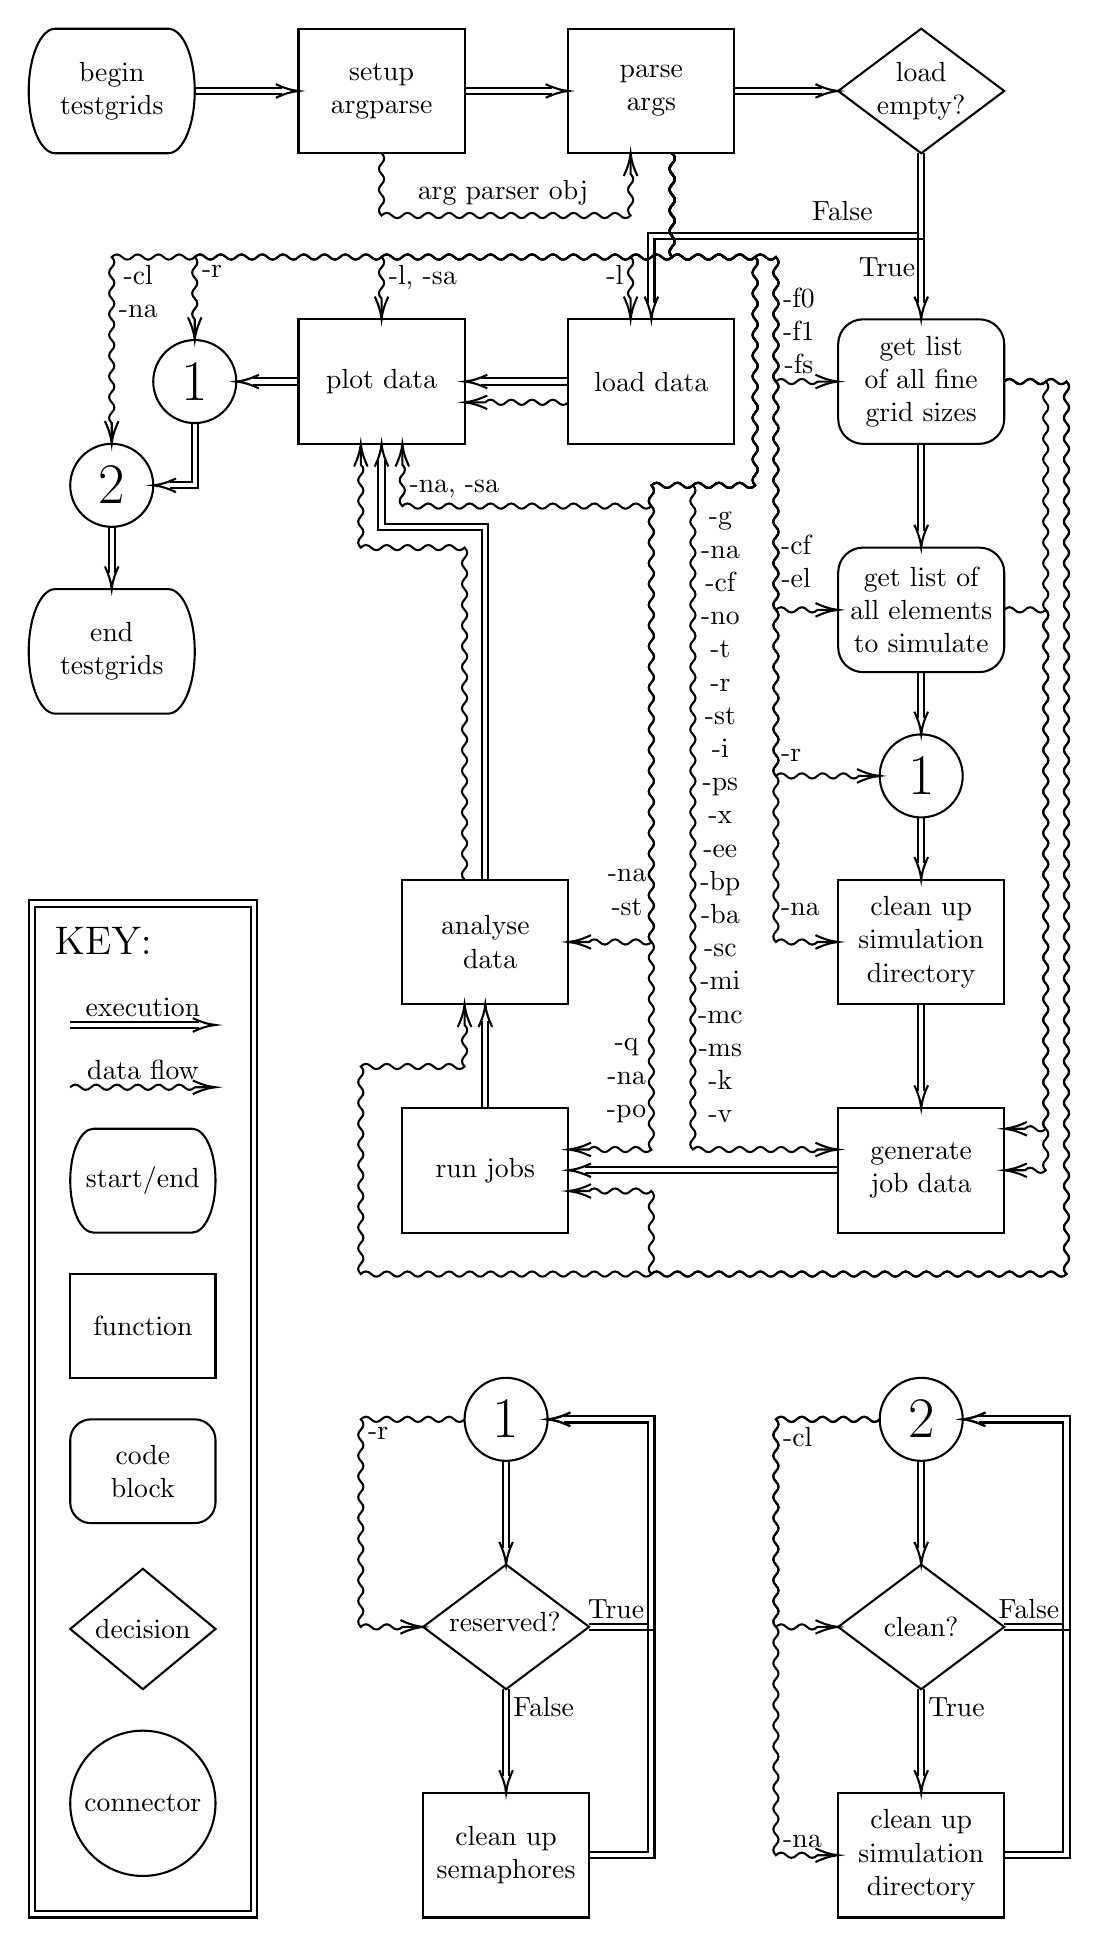
\begin{tikzpicture}[x=0.75pt,y=0.75pt,yscale=-1,xscale=1]
%uncomment if require: \path (0,1077); %set diagram left start at 0, and has height of 1077

%Flowchart: Terminator [id:dp25827733308351086] 
\draw   (22.8,20) -- (77.2,20) .. controls (84.27,20) and (90,33.43) .. (90,50) .. controls (90,66.57) and (84.27,80) .. (77.2,80) -- (22.8,80) .. controls (15.73,80) and (10,66.57) .. (10,50) .. controls (10,33.43) and (15.73,20) .. (22.8,20) -- cycle ;
%Flowchart: Process [id:dp3688925399768985] 
\draw   (140,20) -- (220,20) -- (220,80) -- (140,80) -- cycle ;
%Straight Lines [id:da6785693669659618] 
\draw    (90,48.5) -- (132,48.5)(90,51.5) -- (132,51.5) ;
\draw [shift={(140,50)}, rotate = 180] [color={rgb, 255:red, 0; green, 0; blue, 0 }  ][line width=0.75]    (10.93,-3.29) .. controls (6.95,-1.4) and (3.31,-0.3) .. (0,0) .. controls (3.31,0.3) and (6.95,1.4) .. (10.93,3.29)   ;
%Flowchart: Process [id:dp4463493650567436] 
\draw   (270,20) -- (350,20) -- (350,80) -- (270,80) -- cycle ;
%Straight Lines [id:da587545871050758] 
\draw    (220,48.5) -- (262,48.5)(220,51.5) -- (262,51.5) ;
\draw [shift={(270,50)}, rotate = 180] [color={rgb, 255:red, 0; green, 0; blue, 0 }  ][line width=0.75]    (10.93,-3.29) .. controls (6.95,-1.4) and (3.31,-0.3) .. (0,0) .. controls (3.31,0.3) and (6.95,1.4) .. (10.93,3.29)   ;
%Straight Lines [id:da013992304833393643] 
\draw    (180,80) .. controls (181.67,81.67) and (181.67,83.33) .. (180,85) .. controls (178.33,86.67) and (178.33,88.33) .. (180,90) .. controls (181.67,91.67) and (181.67,93.33) .. (180,95) .. controls (178.33,96.67) and (178.33,98.33) .. (180,100) .. controls (181.67,101.67) and (181.67,103.33) .. (180,105) .. controls (178.33,106.67) and (178.33,108.33) .. (180,110) -- (180,110) .. controls (181.67,108.33) and (183.33,108.33) .. (185,110) .. controls (186.67,111.67) and (188.33,111.67) .. (190,110) .. controls (191.67,108.33) and (193.33,108.33) .. (195,110) .. controls (196.67,111.67) and (198.33,111.67) .. (200,110) .. controls (201.67,108.33) and (203.33,108.33) .. (205,110) .. controls (206.67,111.67) and (208.33,111.67) .. (210,110) .. controls (211.67,108.33) and (213.33,108.33) .. (215,110) .. controls (216.67,111.67) and (218.33,111.67) .. (220,110) .. controls (221.67,108.33) and (223.33,108.33) .. (225,110) .. controls (226.67,111.67) and (228.33,111.67) .. (230,110) .. controls (231.67,108.33) and (233.33,108.33) .. (235,110) .. controls (236.67,111.67) and (238.33,111.67) .. (240,110) .. controls (241.67,108.33) and (243.33,108.33) .. (245,110) .. controls (246.67,111.67) and (248.33,111.67) .. (250,110) .. controls (251.67,108.33) and (253.33,108.33) .. (255,110) .. controls (256.67,111.67) and (258.33,111.67) .. (260,110) .. controls (261.67,108.33) and (263.33,108.33) .. (265,110) .. controls (266.67,111.67) and (268.33,111.67) .. (270,110) .. controls (271.67,108.33) and (273.33,108.33) .. (275,110) .. controls (276.67,111.67) and (278.33,111.67) .. (280,110) .. controls (281.67,108.33) and (283.33,108.33) .. (285,110) .. controls (286.67,111.67) and (288.33,111.67) .. (290,110) .. controls (291.67,108.33) and (293.33,108.33) .. (295,110) .. controls (296.67,111.67) and (298.33,111.67) .. (300,110) -- (300,110) .. controls (298.33,108.33) and (298.33,106.67) .. (300,105) .. controls (301.67,103.33) and (301.67,101.67) .. (300,100) .. controls (298.33,98.33) and (298.33,96.67) .. (300,95) .. controls (301.67,93.33) and (301.67,91.67) .. (300,90) -- (300,82) ;
\draw [shift={(300,80)}, rotate = 450] [color={rgb, 255:red, 0; green, 0; blue, 0 }  ][line width=0.75]    (10.93,-3.29) .. controls (6.95,-1.4) and (3.31,-0.3) .. (0,0) .. controls (3.31,0.3) and (6.95,1.4) .. (10.93,3.29)   ;
%Rounded Rect [id:dp6161067588258142] 
\draw   (400,172) .. controls (400,165.37) and (405.37,160) .. (412,160) -- (468,160) .. controls (474.63,160) and (480,165.37) .. (480,172) -- (480,208) .. controls (480,214.63) and (474.63,220) .. (468,220) -- (412,220) .. controls (405.37,220) and (400,214.63) .. (400,208) -- cycle ;
%Straight Lines [id:da9176152285320409] 
\draw    (441.5,330) -- (441.5,352)(438.5,330) -- (438.5,352) ;
\draw [shift={(440,360)}, rotate = 270] [color={rgb, 255:red, 0; green, 0; blue, 0 }  ][line width=0.75]    (10.93,-3.29) .. controls (6.95,-1.4) and (3.31,-0.3) .. (0,0) .. controls (3.31,0.3) and (6.95,1.4) .. (10.93,3.29)   ;
%Straight Lines [id:da15101297008906855] 
\draw    (320,80) .. controls (321.67,81.67) and (321.67,83.33) .. (320,85) .. controls (318.33,86.67) and (318.33,88.33) .. (320,90) .. controls (321.67,91.67) and (321.67,93.33) .. (320,95) .. controls (318.33,96.67) and (318.33,98.33) .. (320,100) .. controls (321.67,101.67) and (321.67,103.33) .. (320,105) .. controls (318.33,106.67) and (318.33,108.33) .. (320,110) .. controls (321.67,111.67) and (321.67,113.33) .. (320,115) .. controls (318.33,116.67) and (318.33,118.33) .. (320,120) .. controls (321.67,121.67) and (321.67,123.33) .. (320,125) .. controls (318.33,126.67) and (318.33,128.33) .. (320,130) -- (320,130) .. controls (321.67,128.33) and (323.33,128.33) .. (325,130) .. controls (326.67,131.67) and (328.33,131.67) .. (330,130) .. controls (331.67,128.33) and (333.33,128.33) .. (335,130) .. controls (336.67,131.67) and (338.33,131.67) .. (340,130) .. controls (341.67,128.33) and (343.33,128.33) .. (345,130) .. controls (346.67,131.67) and (348.33,131.67) .. (350,130) .. controls (351.67,128.33) and (353.33,128.33) .. (355,130) .. controls (356.67,131.67) and (358.33,131.67) .. (360,130) .. controls (361.67,128.33) and (363.33,128.33) .. (365,130) .. controls (366.67,131.67) and (368.33,131.67) .. (370,130) -- (370,130) .. controls (371.67,131.67) and (371.67,133.33) .. (370,135) .. controls (368.33,136.67) and (368.33,138.33) .. (370,140) .. controls (371.67,141.67) and (371.67,143.33) .. (370,145) .. controls (368.33,146.67) and (368.33,148.33) .. (370,150) .. controls (371.67,151.67) and (371.67,153.33) .. (370,155) .. controls (368.33,156.67) and (368.33,158.33) .. (370,160) .. controls (371.67,161.67) and (371.67,163.33) .. (370,165) .. controls (368.33,166.67) and (368.33,168.33) .. (370,170) .. controls (371.67,171.67) and (371.67,173.33) .. (370,175) .. controls (368.33,176.67) and (368.33,178.33) .. (370,180) .. controls (371.67,181.67) and (371.67,183.33) .. (370,185) .. controls (368.33,186.67) and (368.33,188.33) .. (370,190) -- (370,190) .. controls (371.67,188.33) and (373.33,188.33) .. (375,190) .. controls (376.67,191.67) and (378.33,191.67) .. (380,190) .. controls (381.67,188.33) and (383.33,188.33) .. (385,190) .. controls (386.67,191.67) and (388.33,191.67) .. (390,190) -- (398,190) ;
\draw [shift={(400,190)}, rotate = 180] [color={rgb, 255:red, 0; green, 0; blue, 0 }  ][line width=0.75]    (10.93,-3.29) .. controls (6.95,-1.4) and (3.31,-0.3) .. (0,0) .. controls (3.31,0.3) and (6.95,1.4) .. (10.93,3.29)   ;
%Rounded Rect [id:dp3908718023644233] 
\draw   (400,282) .. controls (400,275.37) and (405.37,270) .. (412,270) -- (468,270) .. controls (474.63,270) and (480,275.37) .. (480,282) -- (480,318) .. controls (480,324.63) and (474.63,330) .. (468,330) -- (412,330) .. controls (405.37,330) and (400,324.63) .. (400,318) -- cycle ;
%Straight Lines [id:da831321020660418] 
\draw    (441.5,220) -- (441.5,262)(438.5,220) -- (438.5,262) ;
\draw [shift={(440,270)}, rotate = 270] [color={rgb, 255:red, 0; green, 0; blue, 0 }  ][line width=0.75]    (10.93,-3.29) .. controls (6.95,-1.4) and (3.31,-0.3) .. (0,0) .. controls (3.31,0.3) and (6.95,1.4) .. (10.93,3.29)   ;
%Straight Lines [id:da9896140948972061] 
\draw    (320,80) .. controls (321.67,81.67) and (321.67,83.33) .. (320,85) .. controls (318.33,86.67) and (318.33,88.33) .. (320,90) .. controls (321.67,91.67) and (321.67,93.33) .. (320,95) .. controls (318.33,96.67) and (318.33,98.33) .. (320,100) .. controls (321.67,101.67) and (321.67,103.33) .. (320,105) .. controls (318.33,106.67) and (318.33,108.33) .. (320,110) .. controls (321.67,111.67) and (321.67,113.33) .. (320,115) .. controls (318.33,116.67) and (318.33,118.33) .. (320,120) .. controls (321.67,121.67) and (321.67,123.33) .. (320,125) .. controls (318.33,126.67) and (318.33,128.33) .. (320,130) -- (320,130) .. controls (321.67,128.33) and (323.33,128.33) .. (325,130) .. controls (326.67,131.67) and (328.33,131.67) .. (330,130) .. controls (331.67,128.33) and (333.33,128.33) .. (335,130) .. controls (336.67,131.67) and (338.33,131.67) .. (340,130) .. controls (341.67,128.33) and (343.33,128.33) .. (345,130) .. controls (346.67,131.67) and (348.33,131.67) .. (350,130) .. controls (351.67,128.33) and (353.33,128.33) .. (355,130) .. controls (356.67,131.67) and (358.33,131.67) .. (360,130) .. controls (361.67,128.33) and (363.33,128.33) .. (365,130) .. controls (366.67,131.67) and (368.33,131.67) .. (370,130) -- (370,130) .. controls (371.67,131.67) and (371.67,133.33) .. (370,135) .. controls (368.33,136.67) and (368.33,138.33) .. (370,140) .. controls (371.67,141.67) and (371.67,143.33) .. (370,145) .. controls (368.33,146.67) and (368.33,148.33) .. (370,150) .. controls (371.67,151.67) and (371.67,153.33) .. (370,155) .. controls (368.33,156.67) and (368.33,158.33) .. (370,160) .. controls (371.67,161.67) and (371.67,163.33) .. (370,165) .. controls (368.33,166.67) and (368.33,168.33) .. (370,170) .. controls (371.67,171.67) and (371.67,173.33) .. (370,175) .. controls (368.33,176.67) and (368.33,178.33) .. (370,180) .. controls (371.67,181.67) and (371.67,183.33) .. (370,185) .. controls (368.33,186.67) and (368.33,188.33) .. (370,190) .. controls (371.67,191.67) and (371.67,193.33) .. (370,195) .. controls (368.33,196.67) and (368.33,198.33) .. (370,200) .. controls (371.67,201.67) and (371.67,203.33) .. (370,205) .. controls (368.33,206.67) and (368.33,208.33) .. (370,210) .. controls (371.67,211.67) and (371.67,213.33) .. (370,215) .. controls (368.33,216.67) and (368.33,218.33) .. (370,220) .. controls (371.67,221.67) and (371.67,223.33) .. (370,225) .. controls (368.33,226.67) and (368.33,228.33) .. (370,230) .. controls (371.67,231.67) and (371.67,233.33) .. (370,235) .. controls (368.33,236.67) and (368.33,238.33) .. (370,240) .. controls (371.67,241.67) and (371.67,243.33) .. (370,245) .. controls (368.33,246.67) and (368.33,248.33) .. (370,250) .. controls (371.67,251.67) and (371.67,253.33) .. (370,255) .. controls (368.33,256.67) and (368.33,258.33) .. (370,260) .. controls (371.67,261.67) and (371.67,263.33) .. (370,265) .. controls (368.33,266.67) and (368.33,268.33) .. (370,270) .. controls (371.67,271.67) and (371.67,273.33) .. (370,275) .. controls (368.33,276.67) and (368.33,278.33) .. (370,280) .. controls (371.67,281.67) and (371.67,283.33) .. (370,285) .. controls (368.33,286.67) and (368.33,288.33) .. (370,290) .. controls (371.67,291.67) and (371.67,293.33) .. (370,295) .. controls (368.33,296.67) and (368.33,298.33) .. (370,300) -- (370,300) .. controls (371.67,298.33) and (373.33,298.33) .. (375,300) .. controls (376.67,301.67) and (378.33,301.67) .. (380,300) .. controls (381.67,298.33) and (383.33,298.33) .. (385,300) .. controls (386.67,301.67) and (388.33,301.67) .. (390,300) -- (398,300) ;
\draw [shift={(400,300)}, rotate = 180] [color={rgb, 255:red, 0; green, 0; blue, 0 }  ][line width=0.75]    (10.93,-3.29) .. controls (6.95,-1.4) and (3.31,-0.3) .. (0,0) .. controls (3.31,0.3) and (6.95,1.4) .. (10.93,3.29)   ;
%Flowchart: Process [id:dp8973254912651609] 
\draw   (400,430) -- (480,430) -- (480,490) -- (400,490) -- cycle ;
%Straight Lines [id:da1959957102853911] 
\draw    (441.5,400) -- (441.5,422)(438.5,400) -- (438.5,422) ;
\draw [shift={(440,430)}, rotate = 270] [color={rgb, 255:red, 0; green, 0; blue, 0 }  ][line width=0.75]    (10.93,-3.29) .. controls (6.95,-1.4) and (3.31,-0.3) .. (0,0) .. controls (3.31,0.3) and (6.95,1.4) .. (10.93,3.29)   ;
%Flowchart: Process [id:dp7105585247007951] 
\draw   (400,540) -- (480,540) -- (480,600) -- (400,600) -- cycle ;
%Straight Lines [id:da08736456972522966] 
\draw    (441.5,490) -- (441.5,532)(438.5,490) -- (438.5,532) ;
\draw [shift={(440,540)}, rotate = 270] [color={rgb, 255:red, 0; green, 0; blue, 0 }  ][line width=0.75]    (10.93,-3.29) .. controls (6.95,-1.4) and (3.31,-0.3) .. (0,0) .. controls (3.31,0.3) and (6.95,1.4) .. (10.93,3.29)   ;
%Straight Lines [id:da9622124136459747] 
\draw    (480,190) .. controls (481.67,188.33) and (483.33,188.33) .. (485,190) .. controls (486.67,191.67) and (488.33,191.67) .. (490,190) .. controls (491.67,188.33) and (493.33,188.33) .. (495,190) .. controls (496.67,191.67) and (498.33,191.67) .. (500,190) -- (500,190) .. controls (501.67,191.67) and (501.67,193.33) .. (500,195) .. controls (498.33,196.67) and (498.33,198.33) .. (500,200) .. controls (501.67,201.67) and (501.67,203.33) .. (500,205) .. controls (498.33,206.67) and (498.33,208.33) .. (500,210) .. controls (501.67,211.67) and (501.67,213.33) .. (500,215) .. controls (498.33,216.67) and (498.33,218.33) .. (500,220) .. controls (501.67,221.67) and (501.67,223.33) .. (500,225) .. controls (498.33,226.67) and (498.33,228.33) .. (500,230) .. controls (501.67,231.67) and (501.67,233.33) .. (500,235) .. controls (498.33,236.67) and (498.33,238.33) .. (500,240) .. controls (501.67,241.67) and (501.67,243.33) .. (500,245) .. controls (498.33,246.67) and (498.33,248.33) .. (500,250) .. controls (501.67,251.67) and (501.67,253.33) .. (500,255) .. controls (498.33,256.67) and (498.33,258.33) .. (500,260) .. controls (501.67,261.67) and (501.67,263.33) .. (500,265) .. controls (498.33,266.67) and (498.33,268.33) .. (500,270) .. controls (501.67,271.67) and (501.67,273.33) .. (500,275) .. controls (498.33,276.67) and (498.33,278.33) .. (500,280) .. controls (501.67,281.67) and (501.67,283.33) .. (500,285) .. controls (498.33,286.67) and (498.33,288.33) .. (500,290) .. controls (501.67,291.67) and (501.67,293.33) .. (500,295) .. controls (498.33,296.67) and (498.33,298.33) .. (500,300) .. controls (501.67,301.67) and (501.67,303.33) .. (500,305) .. controls (498.33,306.67) and (498.33,308.33) .. (500,310) .. controls (501.67,311.67) and (501.67,313.33) .. (500,315) .. controls (498.33,316.67) and (498.33,318.33) .. (500,320) .. controls (501.67,321.67) and (501.67,323.33) .. (500,325) .. controls (498.33,326.67) and (498.33,328.33) .. (500,330) .. controls (501.67,331.67) and (501.67,333.33) .. (500,335) .. controls (498.33,336.67) and (498.33,338.33) .. (500,340) .. controls (501.67,341.67) and (501.67,343.33) .. (500,345) .. controls (498.33,346.67) and (498.33,348.33) .. (500,350) .. controls (501.67,351.67) and (501.67,353.33) .. (500,355) .. controls (498.33,356.67) and (498.33,358.33) .. (500,360) .. controls (501.67,361.67) and (501.67,363.33) .. (500,365) .. controls (498.33,366.67) and (498.33,368.33) .. (500,370) .. controls (501.67,371.67) and (501.67,373.33) .. (500,375) .. controls (498.33,376.67) and (498.33,378.33) .. (500,380) .. controls (501.67,381.67) and (501.67,383.33) .. (500,385) .. controls (498.33,386.67) and (498.33,388.33) .. (500,390) .. controls (501.67,391.67) and (501.67,393.33) .. (500,395) .. controls (498.33,396.67) and (498.33,398.33) .. (500,400) .. controls (501.67,401.67) and (501.67,403.33) .. (500,405) .. controls (498.33,406.67) and (498.33,408.33) .. (500,410) .. controls (501.67,411.67) and (501.67,413.33) .. (500,415) .. controls (498.33,416.67) and (498.33,418.33) .. (500,420) .. controls (501.67,421.67) and (501.67,423.33) .. (500,425) .. controls (498.33,426.67) and (498.33,428.33) .. (500,430) .. controls (501.67,431.67) and (501.67,433.33) .. (500,435) .. controls (498.33,436.67) and (498.33,438.33) .. (500,440) .. controls (501.67,441.67) and (501.67,443.33) .. (500,445) .. controls (498.33,446.67) and (498.33,448.33) .. (500,450) .. controls (501.67,451.67) and (501.67,453.33) .. (500,455) .. controls (498.33,456.67) and (498.33,458.33) .. (500,460) .. controls (501.67,461.67) and (501.67,463.33) .. (500,465) .. controls (498.33,466.67) and (498.33,468.33) .. (500,470) .. controls (501.67,471.67) and (501.67,473.33) .. (500,475) .. controls (498.33,476.67) and (498.33,478.33) .. (500,480) .. controls (501.67,481.67) and (501.67,483.33) .. (500,485) .. controls (498.33,486.67) and (498.33,488.33) .. (500,490) .. controls (501.67,491.67) and (501.67,493.33) .. (500,495) .. controls (498.33,496.67) and (498.33,498.33) .. (500,500) .. controls (501.67,501.67) and (501.67,503.33) .. (500,505) .. controls (498.33,506.67) and (498.33,508.33) .. (500,510) .. controls (501.67,511.67) and (501.67,513.33) .. (500,515) .. controls (498.33,516.67) and (498.33,518.33) .. (500,520) .. controls (501.67,521.67) and (501.67,523.33) .. (500,525) .. controls (498.33,526.67) and (498.33,528.33) .. (500,530) .. controls (501.67,531.67) and (501.67,533.33) .. (500,535) .. controls (498.33,536.67) and (498.33,538.33) .. (500,540) .. controls (501.67,541.67) and (501.67,543.33) .. (500,545) .. controls (498.33,546.67) and (498.33,548.33) .. (500,550) -- (500,550) .. controls (498.33,551.67) and (496.67,551.67) .. (495,550) .. controls (493.33,548.33) and (491.67,548.33) .. (490,550) -- (482,550) ;
\draw [shift={(480,550)}, rotate = 360] [color={rgb, 255:red, 0; green, 0; blue, 0 }  ][line width=0.75]    (10.93,-3.29) .. controls (6.95,-1.4) and (3.31,-0.3) .. (0,0) .. controls (3.31,0.3) and (6.95,1.4) .. (10.93,3.29)   ;
%Flowchart: Process [id:dp45055516879430413] 
\draw   (190,540) -- (270,540) -- (270,600) -- (190,600) -- cycle ;
%Straight Lines [id:da46763617560978665] 
\draw    (400,571.5) -- (278,571.5)(400,568.5) -- (278,568.5) ;
\draw [shift={(270,570)}, rotate = 360] [color={rgb, 255:red, 0; green, 0; blue, 0 }  ][line width=0.75]    (10.93,-3.29) .. controls (6.95,-1.4) and (3.31,-0.3) .. (0,0) .. controls (3.31,0.3) and (6.95,1.4) .. (10.93,3.29)   ;
%Flowchart: Process [id:dp6168087151963813] 
\draw   (190,430) -- (270,430) -- (270,490) -- (190,490) -- cycle ;
%Straight Lines [id:da6266302571004723] 
\draw    (228.5,540) -- (228.5,498)(231.5,540) -- (231.5,498) ;
\draw [shift={(230,490)}, rotate = 450] [color={rgb, 255:red, 0; green, 0; blue, 0 }  ][line width=0.75]    (10.93,-3.29) .. controls (6.95,-1.4) and (3.31,-0.3) .. (0,0) .. controls (3.31,0.3) and (6.95,1.4) .. (10.93,3.29)   ;
%Flowchart: Process [id:dp14256011170842764] 
\draw   (140,160) -- (220,160) -- (220,220) -- (140,220) -- cycle ;
%Straight Lines [id:da5667079663431713] 
\draw    (228.5,430) -- (228.5,261.5) -- (178.5,261.5) -- (178.5,228)(231.5,430) -- (231.5,258.5) -- (181.5,258.5) -- (181.5,228) ;
\draw [shift={(180,220)}, rotate = 450] [color={rgb, 255:red, 0; green, 0; blue, 0 }  ][line width=0.75]    (10.93,-3.29) .. controls (6.95,-1.4) and (3.31,-0.3) .. (0,0) .. controls (3.31,0.3) and (6.95,1.4) .. (10.93,3.29)   ;
%Straight Lines [id:da26600828828569156] 
\draw    (220,430) .. controls (218.33,428.33) and (218.33,426.67) .. (220,425) .. controls (221.67,423.33) and (221.67,421.67) .. (220,420) .. controls (218.33,418.33) and (218.33,416.67) .. (220,415) .. controls (221.67,413.33) and (221.67,411.67) .. (220,410) .. controls (218.33,408.33) and (218.33,406.67) .. (220,405) .. controls (221.67,403.33) and (221.67,401.67) .. (220,400) .. controls (218.33,398.33) and (218.33,396.67) .. (220,395) .. controls (221.67,393.33) and (221.67,391.67) .. (220,390) .. controls (218.33,388.33) and (218.33,386.67) .. (220,385) .. controls (221.67,383.33) and (221.67,381.67) .. (220,380) .. controls (218.33,378.33) and (218.33,376.67) .. (220,375) .. controls (221.67,373.33) and (221.67,371.67) .. (220,370) .. controls (218.33,368.33) and (218.33,366.67) .. (220,365) .. controls (221.67,363.33) and (221.67,361.67) .. (220,360) .. controls (218.33,358.33) and (218.33,356.67) .. (220,355) .. controls (221.67,353.33) and (221.67,351.67) .. (220,350) .. controls (218.33,348.33) and (218.33,346.67) .. (220,345) .. controls (221.67,343.33) and (221.67,341.67) .. (220,340) .. controls (218.33,338.33) and (218.33,336.67) .. (220,335) .. controls (221.67,333.33) and (221.67,331.67) .. (220,330) .. controls (218.33,328.33) and (218.33,326.67) .. (220,325) .. controls (221.67,323.33) and (221.67,321.67) .. (220,320) .. controls (218.33,318.33) and (218.33,316.67) .. (220,315) .. controls (221.67,313.33) and (221.67,311.67) .. (220,310) .. controls (218.33,308.33) and (218.33,306.67) .. (220,305) .. controls (221.67,303.33) and (221.67,301.67) .. (220,300) .. controls (218.33,298.33) and (218.33,296.67) .. (220,295) .. controls (221.67,293.33) and (221.67,291.67) .. (220,290) .. controls (218.33,288.33) and (218.33,286.67) .. (220,285) .. controls (221.67,283.33) and (221.67,281.67) .. (220,280) .. controls (218.33,278.33) and (218.33,276.67) .. (220,275) .. controls (221.67,273.33) and (221.67,271.67) .. (220,270) -- (220,270) .. controls (218.33,271.67) and (216.67,271.67) .. (215,270) .. controls (213.33,268.33) and (211.67,268.33) .. (210,270) .. controls (208.33,271.67) and (206.67,271.67) .. (205,270) .. controls (203.33,268.33) and (201.67,268.33) .. (200,270) .. controls (198.33,271.67) and (196.67,271.67) .. (195,270) .. controls (193.33,268.33) and (191.67,268.33) .. (190,270) .. controls (188.33,271.67) and (186.67,271.67) .. (185,270) .. controls (183.33,268.33) and (181.67,268.33) .. (180,270) .. controls (178.33,271.67) and (176.67,271.67) .. (175,270) .. controls (173.33,268.33) and (171.67,268.33) .. (170,270) -- (170,270) .. controls (168.33,268.33) and (168.33,266.67) .. (170,265) .. controls (171.67,263.33) and (171.67,261.67) .. (170,260) .. controls (168.33,258.33) and (168.33,256.67) .. (170,255) .. controls (171.67,253.33) and (171.67,251.67) .. (170,250) .. controls (168.33,248.33) and (168.33,246.67) .. (170,245) .. controls (171.67,243.33) and (171.67,241.67) .. (170,240) .. controls (168.33,238.33) and (168.33,236.67) .. (170,235) .. controls (171.67,233.33) and (171.67,231.67) .. (170,230) -- (170,222) ;
\draw [shift={(170,220)}, rotate = 450] [color={rgb, 255:red, 0; green, 0; blue, 0 }  ][line width=0.75]    (10.93,-3.29) .. controls (6.95,-1.4) and (3.31,-0.3) .. (0,0) .. controls (3.31,0.3) and (6.95,1.4) .. (10.93,3.29)   ;
%Flowchart: Process [id:dp8748177096856669] 
\draw   (270,160) -- (350,160) -- (350,220) -- (270,220) -- cycle ;
%Straight Lines [id:da9573981618254621] 
\draw    (270,191.5) -- (228,191.5)(270,188.5) -- (228,188.5) ;
\draw [shift={(220,190)}, rotate = 360] [color={rgb, 255:red, 0; green, 0; blue, 0 }  ][line width=0.75]    (10.93,-3.29) .. controls (6.95,-1.4) and (3.31,-0.3) .. (0,0) .. controls (3.31,0.3) and (6.95,1.4) .. (10.93,3.29)   ;
%Straight Lines [id:da7618093809472319] 
\draw    (441.5,80) -- (441.5,121.5) -- (311.5,121.5) -- (311.5,152)(438.5,80) -- (438.5,118.5) -- (308.5,118.5) -- (308.5,152) ;
\draw [shift={(310,160)}, rotate = 270] [color={rgb, 255:red, 0; green, 0; blue, 0 }  ][line width=0.75]    (10.93,-3.29) .. controls (6.95,-1.4) and (3.31,-0.3) .. (0,0) .. controls (3.31,0.3) and (6.95,1.4) .. (10.93,3.29)   ;
%Flowchart: Terminator [id:dp6533098311473264] 
\draw   (22.8,290) -- (77.2,290) .. controls (84.27,290) and (90,303.43) .. (90,320) .. controls (90,336.57) and (84.27,350) .. (77.2,350) -- (22.8,350) .. controls (15.73,350) and (10,336.57) .. (10,320) .. controls (10,303.43) and (15.73,290) .. (22.8,290) -- cycle ;
%Shape: Diamond [id:dp27764507055785814] 
\draw   (440,20) -- (480,50) -- (440,80) -- (400,50) -- cycle ;
%Straight Lines [id:da6003915495028687] 
\draw    (350,48.5) -- (392,48.5)(350,51.5) -- (392,51.5) ;
\draw [shift={(400,50)}, rotate = 180] [color={rgb, 255:red, 0; green, 0; blue, 0 }  ][line width=0.75]    (10.93,-3.29) .. controls (6.95,-1.4) and (3.31,-0.3) .. (0,0) .. controls (3.31,0.3) and (6.95,1.4) .. (10.93,3.29)   ;
%Straight Lines [id:da928423032664172] 
\draw    (441.5,80) -- (441.5,152)(438.5,80) -- (438.5,152) ;
\draw [shift={(440,160)}, rotate = 270] [color={rgb, 255:red, 0; green, 0; blue, 0 }  ][line width=0.75]    (10.93,-3.29) .. controls (6.95,-1.4) and (3.31,-0.3) .. (0,0) .. controls (3.31,0.3) and (6.95,1.4) .. (10.93,3.29)   ;
%Straight Lines [id:da30165885274052173] 
\draw    (320,80) .. controls (321.67,81.67) and (321.67,83.33) .. (320,85) .. controls (318.33,86.67) and (318.33,88.33) .. (320,90) .. controls (321.67,91.67) and (321.67,93.33) .. (320,95) .. controls (318.33,96.67) and (318.33,98.33) .. (320,100) .. controls (321.67,101.67) and (321.67,103.33) .. (320,105) .. controls (318.33,106.67) and (318.33,108.33) .. (320,110) .. controls (321.67,111.67) and (321.67,113.33) .. (320,115) .. controls (318.33,116.67) and (318.33,118.33) .. (320,120) .. controls (321.67,121.67) and (321.67,123.33) .. (320,125) .. controls (318.33,126.67) and (318.33,128.33) .. (320,130) -- (320,130) .. controls (318.33,131.67) and (316.67,131.67) .. (315,130) .. controls (313.33,128.33) and (311.67,128.33) .. (310,130) .. controls (308.33,131.67) and (306.67,131.67) .. (305,130) .. controls (303.33,128.33) and (301.67,128.33) .. (300,130) -- (300,130) .. controls (301.67,131.67) and (301.67,133.33) .. (300,135) .. controls (298.33,136.67) and (298.33,138.33) .. (300,140) .. controls (301.67,141.67) and (301.67,143.33) .. (300,145) .. controls (298.33,146.67) and (298.33,148.33) .. (300,150) -- (300,158) ;
\draw [shift={(300,160)}, rotate = 270] [color={rgb, 255:red, 0; green, 0; blue, 0 }  ][line width=0.75]    (10.93,-3.29) .. controls (6.95,-1.4) and (3.31,-0.3) .. (0,0) .. controls (3.31,0.3) and (6.95,1.4) .. (10.93,3.29)   ;
%Straight Lines [id:da4984335162646871] 
\draw    (320,80) .. controls (321.67,81.67) and (321.67,83.33) .. (320,85) .. controls (318.33,86.67) and (318.33,88.33) .. (320,90) .. controls (321.67,91.67) and (321.67,93.33) .. (320,95) .. controls (318.33,96.67) and (318.33,98.33) .. (320,100) .. controls (321.67,101.67) and (321.67,103.33) .. (320,105) .. controls (318.33,106.67) and (318.33,108.33) .. (320,110) .. controls (321.67,111.67) and (321.67,113.33) .. (320,115) .. controls (318.33,116.67) and (318.33,118.33) .. (320,120) .. controls (321.67,121.67) and (321.67,123.33) .. (320,125) .. controls (318.33,126.67) and (318.33,128.33) .. (320,130) -- (320,130) .. controls (318.33,131.67) and (316.67,131.67) .. (315,130) .. controls (313.33,128.33) and (311.67,128.33) .. (310,130) .. controls (308.33,131.67) and (306.67,131.67) .. (305,130) .. controls (303.33,128.33) and (301.67,128.33) .. (300,130) .. controls (298.33,131.67) and (296.67,131.67) .. (295,130) .. controls (293.33,128.33) and (291.67,128.33) .. (290,130) .. controls (288.33,131.67) and (286.67,131.67) .. (285,130) .. controls (283.33,128.33) and (281.67,128.33) .. (280,130) .. controls (278.33,131.67) and (276.67,131.67) .. (275,130) .. controls (273.33,128.33) and (271.67,128.33) .. (270,130) .. controls (268.33,131.67) and (266.67,131.67) .. (265,130) .. controls (263.33,128.33) and (261.67,128.33) .. (260,130) .. controls (258.33,131.67) and (256.67,131.67) .. (255,130) .. controls (253.33,128.33) and (251.67,128.33) .. (250,130) .. controls (248.33,131.67) and (246.67,131.67) .. (245,130) .. controls (243.33,128.33) and (241.67,128.33) .. (240,130) .. controls (238.33,131.67) and (236.67,131.67) .. (235,130) .. controls (233.33,128.33) and (231.67,128.33) .. (230,130) .. controls (228.33,131.67) and (226.67,131.67) .. (225,130) .. controls (223.33,128.33) and (221.67,128.33) .. (220,130) .. controls (218.33,131.67) and (216.67,131.67) .. (215,130) .. controls (213.33,128.33) and (211.67,128.33) .. (210,130) .. controls (208.33,131.67) and (206.67,131.67) .. (205,130) .. controls (203.33,128.33) and (201.67,128.33) .. (200,130) .. controls (198.33,131.67) and (196.67,131.67) .. (195,130) .. controls (193.33,128.33) and (191.67,128.33) .. (190,130) .. controls (188.33,131.67) and (186.67,131.67) .. (185,130) .. controls (183.33,128.33) and (181.67,128.33) .. (180,130) -- (180,130) .. controls (181.67,131.67) and (181.67,133.33) .. (180,135) .. controls (178.33,136.67) and (178.33,138.33) .. (180,140) .. controls (181.67,141.67) and (181.67,143.33) .. (180,145) .. controls (178.33,146.67) and (178.33,148.33) .. (180,150) -- (180,158) ;
\draw [shift={(180,160)}, rotate = 270] [color={rgb, 255:red, 0; green, 0; blue, 0 }  ][line width=0.75]    (10.93,-3.29) .. controls (6.95,-1.4) and (3.31,-0.3) .. (0,0) .. controls (3.31,0.3) and (6.95,1.4) .. (10.93,3.29)   ;
%Straight Lines [id:da05715907224214334] 
\draw    (270,200) .. controls (268.33,201.67) and (266.67,201.67) .. (265,200) .. controls (263.33,198.33) and (261.67,198.33) .. (260,200) .. controls (258.33,201.67) and (256.67,201.67) .. (255,200) .. controls (253.33,198.33) and (251.67,198.33) .. (250,200) .. controls (248.33,201.67) and (246.67,201.67) .. (245,200) .. controls (243.33,198.33) and (241.67,198.33) .. (240,200) .. controls (238.33,201.67) and (236.67,201.67) .. (235,200) .. controls (233.33,198.33) and (231.67,198.33) .. (230,200) -- (222,200) ;
\draw [shift={(220,200)}, rotate = 360] [color={rgb, 255:red, 0; green, 0; blue, 0 }  ][line width=0.75]    (10.93,-3.29) .. controls (6.95,-1.4) and (3.31,-0.3) .. (0,0) .. controls (3.31,0.3) and (6.95,1.4) .. (10.93,3.29)   ;
%Flowchart: Connector [id:dp26389314177955536] 
\draw   (220,690) .. controls (220,678.95) and (228.95,670) .. (240,670) .. controls (251.05,670) and (260,678.95) .. (260,690) .. controls (260,701.05) and (251.05,710) .. (240,710) .. controls (228.95,710) and (220,701.05) .. (220,690) -- cycle ;
%Flowchart: Process [id:dp11071382617928749] 
\draw   (200,870) -- (280,870) -- (280,930) -- (200,930) -- cycle ;
%Flowchart: Connector [id:dp2830619650209396] 
\draw   (420,380) .. controls (420,368.95) and (428.95,360) .. (440,360) .. controls (451.05,360) and (460,368.95) .. (460,380) .. controls (460,391.05) and (451.05,400) .. (440,400) .. controls (428.95,400) and (420,391.05) .. (420,380) -- cycle ;
%Straight Lines [id:da6972002649995268] 
\draw    (320,80) .. controls (321.67,81.67) and (321.67,83.33) .. (320,85) .. controls (318.33,86.67) and (318.33,88.33) .. (320,90) .. controls (321.67,91.67) and (321.67,93.33) .. (320,95) .. controls (318.33,96.67) and (318.33,98.33) .. (320,100) .. controls (321.67,101.67) and (321.67,103.33) .. (320,105) .. controls (318.33,106.67) and (318.33,108.33) .. (320,110) .. controls (321.67,111.67) and (321.67,113.33) .. (320,115) .. controls (318.33,116.67) and (318.33,118.33) .. (320,120) .. controls (321.67,121.67) and (321.67,123.33) .. (320,125) .. controls (318.33,126.67) and (318.33,128.33) .. (320,130) -- (320,130) .. controls (321.67,128.33) and (323.33,128.33) .. (325,130) .. controls (326.67,131.67) and (328.33,131.67) .. (330,130) .. controls (331.67,128.33) and (333.33,128.33) .. (335,130) .. controls (336.67,131.67) and (338.33,131.67) .. (340,130) .. controls (341.67,128.33) and (343.33,128.33) .. (345,130) .. controls (346.67,131.67) and (348.33,131.67) .. (350,130) .. controls (351.67,128.33) and (353.33,128.33) .. (355,130) .. controls (356.67,131.67) and (358.33,131.67) .. (360,130) .. controls (361.67,128.33) and (363.33,128.33) .. (365,130) .. controls (366.67,131.67) and (368.33,131.67) .. (370,130) -- (370,130) .. controls (371.67,131.67) and (371.67,133.33) .. (370,135) .. controls (368.33,136.67) and (368.33,138.33) .. (370,140) .. controls (371.67,141.67) and (371.67,143.33) .. (370,145) .. controls (368.33,146.67) and (368.33,148.33) .. (370,150) .. controls (371.67,151.67) and (371.67,153.33) .. (370,155) .. controls (368.33,156.67) and (368.33,158.33) .. (370,160) .. controls (371.67,161.67) and (371.67,163.33) .. (370,165) .. controls (368.33,166.67) and (368.33,168.33) .. (370,170) .. controls (371.67,171.67) and (371.67,173.33) .. (370,175) .. controls (368.33,176.67) and (368.33,178.33) .. (370,180) .. controls (371.67,181.67) and (371.67,183.33) .. (370,185) .. controls (368.33,186.67) and (368.33,188.33) .. (370,190) .. controls (371.67,191.67) and (371.67,193.33) .. (370,195) .. controls (368.33,196.67) and (368.33,198.33) .. (370,200) .. controls (371.67,201.67) and (371.67,203.33) .. (370,205) .. controls (368.33,206.67) and (368.33,208.33) .. (370,210) .. controls (371.67,211.67) and (371.67,213.33) .. (370,215) .. controls (368.33,216.67) and (368.33,218.33) .. (370,220) .. controls (371.67,221.67) and (371.67,223.33) .. (370,225) .. controls (368.33,226.67) and (368.33,228.33) .. (370,230) .. controls (371.67,231.67) and (371.67,233.33) .. (370,235) .. controls (368.33,236.67) and (368.33,238.33) .. (370,240) .. controls (371.67,241.67) and (371.67,243.33) .. (370,245) .. controls (368.33,246.67) and (368.33,248.33) .. (370,250) .. controls (371.67,251.67) and (371.67,253.33) .. (370,255) .. controls (368.33,256.67) and (368.33,258.33) .. (370,260) .. controls (371.67,261.67) and (371.67,263.33) .. (370,265) .. controls (368.33,266.67) and (368.33,268.33) .. (370,270) .. controls (371.67,271.67) and (371.67,273.33) .. (370,275) .. controls (368.33,276.67) and (368.33,278.33) .. (370,280) .. controls (371.67,281.67) and (371.67,283.33) .. (370,285) .. controls (368.33,286.67) and (368.33,288.33) .. (370,290) .. controls (371.67,291.67) and (371.67,293.33) .. (370,295) .. controls (368.33,296.67) and (368.33,298.33) .. (370,300) .. controls (371.67,301.67) and (371.67,303.33) .. (370,305) .. controls (368.33,306.67) and (368.33,308.33) .. (370,310) .. controls (371.67,311.67) and (371.67,313.33) .. (370,315) .. controls (368.33,316.67) and (368.33,318.33) .. (370,320) .. controls (371.67,321.67) and (371.67,323.33) .. (370,325) .. controls (368.33,326.67) and (368.33,328.33) .. (370,330) .. controls (371.67,331.67) and (371.67,333.33) .. (370,335) .. controls (368.33,336.67) and (368.33,338.33) .. (370,340) .. controls (371.67,341.67) and (371.67,343.33) .. (370,345) .. controls (368.33,346.67) and (368.33,348.33) .. (370,350) .. controls (371.67,351.67) and (371.67,353.33) .. (370,355) .. controls (368.33,356.67) and (368.33,358.33) .. (370,360) .. controls (371.67,361.67) and (371.67,363.33) .. (370,365) .. controls (368.33,366.67) and (368.33,368.33) .. (370,370) .. controls (371.67,371.67) and (371.67,373.33) .. (370,375) .. controls (368.33,376.67) and (368.33,378.33) .. (370,380) -- (370,380) .. controls (371.67,378.33) and (373.33,378.33) .. (375,380) .. controls (376.67,381.67) and (378.33,381.67) .. (380,380) .. controls (381.67,378.33) and (383.33,378.33) .. (385,380) .. controls (386.67,381.67) and (388.33,381.67) .. (390,380) .. controls (391.67,378.33) and (393.33,378.33) .. (395,380) .. controls (396.67,381.67) and (398.33,381.67) .. (400,380) .. controls (401.67,378.33) and (403.33,378.33) .. (405,380) .. controls (406.67,381.67) and (408.33,381.67) .. (410,380) -- (418,380) ;
\draw [shift={(420,380)}, rotate = 180] [color={rgb, 255:red, 0; green, 0; blue, 0 }  ][line width=0.75]    (10.93,-3.29) .. controls (6.95,-1.4) and (3.31,-0.3) .. (0,0) .. controls (3.31,0.3) and (6.95,1.4) .. (10.93,3.29)   ;
%Shape: Diamond [id:dp5456840530419882] 
\draw   (240,760) -- (280,790) -- (240,820) -- (200,790) -- cycle ;
%Straight Lines [id:da7657038694742806] 
\draw    (241.5,710) -- (241.5,752)(238.5,710) -- (238.5,752) ;
\draw [shift={(240,760)}, rotate = 270] [color={rgb, 255:red, 0; green, 0; blue, 0 }  ][line width=0.75]    (10.93,-3.29) .. controls (6.95,-1.4) and (3.31,-0.3) .. (0,0) .. controls (3.31,0.3) and (6.95,1.4) .. (10.93,3.29)   ;
%Straight Lines [id:da8441332761159279] 
\draw    (280,788.5) -- (308.5,788.5) -- (308.5,691.5) -- (268,691.5)(280,791.5) -- (311.5,791.5) -- (311.5,688.5) -- (268,688.5) ;
\draw [shift={(260,690)}, rotate = 360] [color={rgb, 255:red, 0; green, 0; blue, 0 }  ][line width=0.75]    (10.93,-3.29) .. controls (6.95,-1.4) and (3.31,-0.3) .. (0,0) .. controls (3.31,0.3) and (6.95,1.4) .. (10.93,3.29)   ;
%Straight Lines [id:da32183636883270794] 
\draw    (220,690) .. controls (218.33,691.67) and (216.67,691.67) .. (215,690) .. controls (213.33,688.33) and (211.67,688.33) .. (210,690) .. controls (208.33,691.67) and (206.67,691.67) .. (205,690) .. controls (203.33,688.33) and (201.67,688.33) .. (200,690) .. controls (198.33,691.67) and (196.67,691.67) .. (195,690) .. controls (193.33,688.33) and (191.67,688.33) .. (190,690) .. controls (188.33,691.67) and (186.67,691.67) .. (185,690) .. controls (183.33,688.33) and (181.67,688.33) .. (180,690) .. controls (178.33,691.67) and (176.67,691.67) .. (175,690) .. controls (173.33,688.33) and (171.67,688.33) .. (170,690) -- (170,690) .. controls (171.67,691.67) and (171.67,693.33) .. (170,695) .. controls (168.33,696.67) and (168.33,698.33) .. (170,700) .. controls (171.67,701.67) and (171.67,703.33) .. (170,705) .. controls (168.33,706.67) and (168.33,708.33) .. (170,710) .. controls (171.67,711.67) and (171.67,713.33) .. (170,715) .. controls (168.33,716.67) and (168.33,718.33) .. (170,720) .. controls (171.67,721.67) and (171.67,723.33) .. (170,725) .. controls (168.33,726.67) and (168.33,728.33) .. (170,730) .. controls (171.67,731.67) and (171.67,733.33) .. (170,735) .. controls (168.33,736.67) and (168.33,738.33) .. (170,740) .. controls (171.67,741.67) and (171.67,743.33) .. (170,745) .. controls (168.33,746.67) and (168.33,748.33) .. (170,750) .. controls (171.67,751.67) and (171.67,753.33) .. (170,755) .. controls (168.33,756.67) and (168.33,758.33) .. (170,760) .. controls (171.67,761.67) and (171.67,763.33) .. (170,765) .. controls (168.33,766.67) and (168.33,768.33) .. (170,770) .. controls (171.67,771.67) and (171.67,773.33) .. (170,775) .. controls (168.33,776.67) and (168.33,778.33) .. (170,780) .. controls (171.67,781.67) and (171.67,783.33) .. (170,785) .. controls (168.33,786.67) and (168.33,788.33) .. (170,790) -- (170,790) .. controls (171.67,788.33) and (173.33,788.33) .. (175,790) .. controls (176.67,791.67) and (178.33,791.67) .. (180,790) .. controls (181.67,788.33) and (183.33,788.33) .. (185,790) .. controls (186.67,791.67) and (188.33,791.67) .. (190,790) -- (198,790) ;
\draw [shift={(200,790)}, rotate = 180] [color={rgb, 255:red, 0; green, 0; blue, 0 }  ][line width=0.75]    (10.93,-3.29) .. controls (6.95,-1.4) and (3.31,-0.3) .. (0,0) .. controls (3.31,0.3) and (6.95,1.4) .. (10.93,3.29)   ;
%Straight Lines [id:da5966644269770032] 
\draw    (241.5,820) -- (241.5,862)(238.5,820) -- (238.5,862) ;
\draw [shift={(240,870)}, rotate = 270] [color={rgb, 255:red, 0; green, 0; blue, 0 }  ][line width=0.75]    (10.93,-3.29) .. controls (6.95,-1.4) and (3.31,-0.3) .. (0,0) .. controls (3.31,0.3) and (6.95,1.4) .. (10.93,3.29)   ;
%Straight Lines [id:da020379736048627306] 
\draw    (280,898.5) -- (308.5,898.5) -- (308.5,691.5) -- (268,691.5)(280,901.5) -- (311.5,901.5) -- (311.5,688.5) -- (268,688.5) ;
\draw [shift={(260,690)}, rotate = 360] [color={rgb, 255:red, 0; green, 0; blue, 0 }  ][line width=0.75]    (10.93,-3.29) .. controls (6.95,-1.4) and (3.31,-0.3) .. (0,0) .. controls (3.31,0.3) and (6.95,1.4) .. (10.93,3.29)   ;
%Straight Lines [id:da6635110663735284] 
\draw    (320,80) .. controls (321.67,81.67) and (321.67,83.33) .. (320,85) .. controls (318.33,86.67) and (318.33,88.33) .. (320,90) .. controls (321.67,91.67) and (321.67,93.33) .. (320,95) .. controls (318.33,96.67) and (318.33,98.33) .. (320,100) .. controls (321.67,101.67) and (321.67,103.33) .. (320,105) .. controls (318.33,106.67) and (318.33,108.33) .. (320,110) .. controls (321.67,111.67) and (321.67,113.33) .. (320,115) .. controls (318.33,116.67) and (318.33,118.33) .. (320,120) .. controls (321.67,121.67) and (321.67,123.33) .. (320,125) .. controls (318.33,126.67) and (318.33,128.33) .. (320,130) -- (320,130) .. controls (321.67,128.33) and (323.33,128.33) .. (325,130) .. controls (326.67,131.67) and (328.33,131.67) .. (330,130) .. controls (331.67,128.33) and (333.33,128.33) .. (335,130) .. controls (336.67,131.67) and (338.33,131.67) .. (340,130) .. controls (341.67,128.33) and (343.33,128.33) .. (345,130) .. controls (346.67,131.67) and (348.33,131.67) .. (350,130) .. controls (351.67,128.33) and (353.33,128.33) .. (355,130) .. controls (356.67,131.67) and (358.33,131.67) .. (360,130) .. controls (361.67,128.33) and (363.33,128.33) .. (365,130) .. controls (366.67,131.67) and (368.33,131.67) .. (370,130) -- (370,130) .. controls (371.67,131.67) and (371.67,133.33) .. (370,135) .. controls (368.33,136.67) and (368.33,138.33) .. (370,140) .. controls (371.67,141.67) and (371.67,143.33) .. (370,145) .. controls (368.33,146.67) and (368.33,148.33) .. (370,150) .. controls (371.67,151.67) and (371.67,153.33) .. (370,155) .. controls (368.33,156.67) and (368.33,158.33) .. (370,160) .. controls (371.67,161.67) and (371.67,163.33) .. (370,165) .. controls (368.33,166.67) and (368.33,168.33) .. (370,170) .. controls (371.67,171.67) and (371.67,173.33) .. (370,175) .. controls (368.33,176.67) and (368.33,178.33) .. (370,180) .. controls (371.67,181.67) and (371.67,183.33) .. (370,185) .. controls (368.33,186.67) and (368.33,188.33) .. (370,190) .. controls (371.67,191.67) and (371.67,193.33) .. (370,195) .. controls (368.33,196.67) and (368.33,198.33) .. (370,200) .. controls (371.67,201.67) and (371.67,203.33) .. (370,205) .. controls (368.33,206.67) and (368.33,208.33) .. (370,210) .. controls (371.67,211.67) and (371.67,213.33) .. (370,215) .. controls (368.33,216.67) and (368.33,218.33) .. (370,220) .. controls (371.67,221.67) and (371.67,223.33) .. (370,225) .. controls (368.33,226.67) and (368.33,228.33) .. (370,230) .. controls (371.67,231.67) and (371.67,233.33) .. (370,235) .. controls (368.33,236.67) and (368.33,238.33) .. (370,240) .. controls (371.67,241.67) and (371.67,243.33) .. (370,245) .. controls (368.33,246.67) and (368.33,248.33) .. (370,250) .. controls (371.67,251.67) and (371.67,253.33) .. (370,255) .. controls (368.33,256.67) and (368.33,258.33) .. (370,260) .. controls (371.67,261.67) and (371.67,263.33) .. (370,265) .. controls (368.33,266.67) and (368.33,268.33) .. (370,270) .. controls (371.67,271.67) and (371.67,273.33) .. (370,275) .. controls (368.33,276.67) and (368.33,278.33) .. (370,280) .. controls (371.67,281.67) and (371.67,283.33) .. (370,285) .. controls (368.33,286.67) and (368.33,288.33) .. (370,290) .. controls (371.67,291.67) and (371.67,293.33) .. (370,295) .. controls (368.33,296.67) and (368.33,298.33) .. (370,300) .. controls (371.67,301.67) and (371.67,303.33) .. (370,305) .. controls (368.33,306.67) and (368.33,308.33) .. (370,310) .. controls (371.67,311.67) and (371.67,313.33) .. (370,315) .. controls (368.33,316.67) and (368.33,318.33) .. (370,320) .. controls (371.67,321.67) and (371.67,323.33) .. (370,325) .. controls (368.33,326.67) and (368.33,328.33) .. (370,330) .. controls (371.67,331.67) and (371.67,333.33) .. (370,335) .. controls (368.33,336.67) and (368.33,338.33) .. (370,340) .. controls (371.67,341.67) and (371.67,343.33) .. (370,345) .. controls (368.33,346.67) and (368.33,348.33) .. (370,350) .. controls (371.67,351.67) and (371.67,353.33) .. (370,355) .. controls (368.33,356.67) and (368.33,358.33) .. (370,360) .. controls (371.67,361.67) and (371.67,363.33) .. (370,365) .. controls (368.33,366.67) and (368.33,368.33) .. (370,370) .. controls (371.67,371.67) and (371.67,373.33) .. (370,375) .. controls (368.33,376.67) and (368.33,378.33) .. (370,380) .. controls (371.67,381.67) and (371.67,383.33) .. (370,385) .. controls (368.33,386.67) and (368.33,388.33) .. (370,390) .. controls (371.67,391.67) and (371.67,393.33) .. (370,395) .. controls (368.33,396.67) and (368.33,398.33) .. (370,400) .. controls (371.67,401.67) and (371.67,403.33) .. (370,405) .. controls (368.33,406.67) and (368.33,408.33) .. (370,410) .. controls (371.67,411.67) and (371.67,413.33) .. (370,415) .. controls (368.33,416.67) and (368.33,418.33) .. (370,420) .. controls (371.67,421.67) and (371.67,423.33) .. (370,425) .. controls (368.33,426.67) and (368.33,428.33) .. (370,430) .. controls (371.67,431.67) and (371.67,433.33) .. (370,435) .. controls (368.33,436.67) and (368.33,438.33) .. (370,440) .. controls (371.67,441.67) and (371.67,443.33) .. (370,445) .. controls (368.33,446.67) and (368.33,448.33) .. (370,450) .. controls (371.67,451.67) and (371.67,453.33) .. (370,455) .. controls (368.33,456.67) and (368.33,458.33) .. (370,460) -- (370,460) .. controls (371.67,458.33) and (373.33,458.33) .. (375,460) .. controls (376.67,461.67) and (378.33,461.67) .. (380,460) .. controls (381.67,458.33) and (383.33,458.33) .. (385,460) .. controls (386.67,461.67) and (388.33,461.67) .. (390,460) -- (398,460) ;
\draw [shift={(400,460)}, rotate = 180] [color={rgb, 255:red, 0; green, 0; blue, 0 }  ][line width=0.75]    (10.93,-3.29) .. controls (6.95,-1.4) and (3.31,-0.3) .. (0,0) .. controls (3.31,0.3) and (6.95,1.4) .. (10.93,3.29)   ;
%Straight Lines [id:da697108539327381] 
\draw    (480,300) .. controls (481.67,298.33) and (483.33,298.33) .. (485,300) .. controls (486.67,301.67) and (488.33,301.67) .. (490,300) .. controls (491.67,298.33) and (493.33,298.33) .. (495,300) .. controls (496.67,301.67) and (498.33,301.67) .. (500,300) -- (500,300) .. controls (501.67,301.67) and (501.67,303.33) .. (500,305) .. controls (498.33,306.67) and (498.33,308.33) .. (500,310) .. controls (501.67,311.67) and (501.67,313.33) .. (500,315) .. controls (498.33,316.67) and (498.33,318.33) .. (500,320) .. controls (501.67,321.67) and (501.67,323.33) .. (500,325) .. controls (498.33,326.67) and (498.33,328.33) .. (500,330) .. controls (501.67,331.67) and (501.67,333.33) .. (500,335) .. controls (498.33,336.67) and (498.33,338.33) .. (500,340) .. controls (501.67,341.67) and (501.67,343.33) .. (500,345) .. controls (498.33,346.67) and (498.33,348.33) .. (500,350) .. controls (501.67,351.67) and (501.67,353.33) .. (500,355) .. controls (498.33,356.67) and (498.33,358.33) .. (500,360) .. controls (501.67,361.67) and (501.67,363.33) .. (500,365) .. controls (498.33,366.67) and (498.33,368.33) .. (500,370) .. controls (501.67,371.67) and (501.67,373.33) .. (500,375) .. controls (498.33,376.67) and (498.33,378.33) .. (500,380) .. controls (501.67,381.67) and (501.67,383.33) .. (500,385) .. controls (498.33,386.67) and (498.33,388.33) .. (500,390) .. controls (501.67,391.67) and (501.67,393.33) .. (500,395) .. controls (498.33,396.67) and (498.33,398.33) .. (500,400) .. controls (501.67,401.67) and (501.67,403.33) .. (500,405) .. controls (498.33,406.67) and (498.33,408.33) .. (500,410) .. controls (501.67,411.67) and (501.67,413.33) .. (500,415) .. controls (498.33,416.67) and (498.33,418.33) .. (500,420) .. controls (501.67,421.67) and (501.67,423.33) .. (500,425) .. controls (498.33,426.67) and (498.33,428.33) .. (500,430) .. controls (501.67,431.67) and (501.67,433.33) .. (500,435) .. controls (498.33,436.67) and (498.33,438.33) .. (500,440) .. controls (501.67,441.67) and (501.67,443.33) .. (500,445) .. controls (498.33,446.67) and (498.33,448.33) .. (500,450) .. controls (501.67,451.67) and (501.67,453.33) .. (500,455) .. controls (498.33,456.67) and (498.33,458.33) .. (500,460) .. controls (501.67,461.67) and (501.67,463.33) .. (500,465) .. controls (498.33,466.67) and (498.33,468.33) .. (500,470) .. controls (501.67,471.67) and (501.67,473.33) .. (500,475) .. controls (498.33,476.67) and (498.33,478.33) .. (500,480) .. controls (501.67,481.67) and (501.67,483.33) .. (500,485) .. controls (498.33,486.67) and (498.33,488.33) .. (500,490) .. controls (501.67,491.67) and (501.67,493.33) .. (500,495) .. controls (498.33,496.67) and (498.33,498.33) .. (500,500) .. controls (501.67,501.67) and (501.67,503.33) .. (500,505) .. controls (498.33,506.67) and (498.33,508.33) .. (500,510) .. controls (501.67,511.67) and (501.67,513.33) .. (500,515) .. controls (498.33,516.67) and (498.33,518.33) .. (500,520) .. controls (501.67,521.67) and (501.67,523.33) .. (500,525) .. controls (498.33,526.67) and (498.33,528.33) .. (500,530) .. controls (501.67,531.67) and (501.67,533.33) .. (500,535) .. controls (498.33,536.67) and (498.33,538.33) .. (500,540) .. controls (501.67,541.67) and (501.67,543.33) .. (500,545) .. controls (498.33,546.67) and (498.33,548.33) .. (500,550) .. controls (501.67,551.67) and (501.67,553.33) .. (500,555) .. controls (498.33,556.67) and (498.33,558.33) .. (500,560) .. controls (501.67,561.67) and (501.67,563.33) .. (500,565) .. controls (498.33,566.67) and (498.33,568.33) .. (500,570) -- (500,570) .. controls (498.33,571.67) and (496.67,571.67) .. (495,570) .. controls (493.33,568.33) and (491.67,568.33) .. (490,570) -- (482,570) ;
\draw [shift={(480,570)}, rotate = 360] [color={rgb, 255:red, 0; green, 0; blue, 0 }  ][line width=0.75]    (10.93,-3.29) .. controls (6.95,-1.4) and (3.31,-0.3) .. (0,0) .. controls (3.31,0.3) and (6.95,1.4) .. (10.93,3.29)   ;
%Straight Lines [id:da7775459067006909] 
\draw    (320,80) .. controls (321.67,81.67) and (321.67,83.33) .. (320,85) .. controls (318.33,86.67) and (318.33,88.33) .. (320,90) .. controls (321.67,91.67) and (321.67,93.33) .. (320,95) .. controls (318.33,96.67) and (318.33,98.33) .. (320,100) .. controls (321.67,101.67) and (321.67,103.33) .. (320,105) .. controls (318.33,106.67) and (318.33,108.33) .. (320,110) .. controls (321.67,111.67) and (321.67,113.33) .. (320,115) .. controls (318.33,116.67) and (318.33,118.33) .. (320,120) .. controls (321.67,121.67) and (321.67,123.33) .. (320,125) .. controls (318.33,126.67) and (318.33,128.33) .. (320,130) -- (320,130) .. controls (321.67,128.33) and (323.33,128.33) .. (325,130) .. controls (326.67,131.67) and (328.33,131.67) .. (330,130) .. controls (331.67,128.33) and (333.33,128.33) .. (335,130) .. controls (336.67,131.67) and (338.33,131.67) .. (340,130) .. controls (341.67,128.33) and (343.33,128.33) .. (345,130) .. controls (346.67,131.67) and (348.33,131.67) .. (350,130) .. controls (351.67,128.33) and (353.33,128.33) .. (355,130) .. controls (356.67,131.67) and (358.33,131.67) .. (360,130) -- (360,130) .. controls (361.67,131.67) and (361.67,133.33) .. (360,135) .. controls (358.33,136.67) and (358.33,138.33) .. (360,140) .. controls (361.67,141.67) and (361.67,143.33) .. (360,145) .. controls (358.33,146.67) and (358.33,148.33) .. (360,150) .. controls (361.67,151.67) and (361.67,153.33) .. (360,155) .. controls (358.33,156.67) and (358.33,158.33) .. (360,160) .. controls (361.67,161.67) and (361.67,163.33) .. (360,165) .. controls (358.33,166.67) and (358.33,168.33) .. (360,170) .. controls (361.67,171.67) and (361.67,173.33) .. (360,175) .. controls (358.33,176.67) and (358.33,178.33) .. (360,180) .. controls (361.67,181.67) and (361.67,183.33) .. (360,185) .. controls (358.33,186.67) and (358.33,188.33) .. (360,190) .. controls (361.67,191.67) and (361.67,193.33) .. (360,195) .. controls (358.33,196.67) and (358.33,198.33) .. (360,200) .. controls (361.67,201.67) and (361.67,203.33) .. (360,205) .. controls (358.33,206.67) and (358.33,208.33) .. (360,210) .. controls (361.67,211.67) and (361.67,213.33) .. (360,215) .. controls (358.33,216.67) and (358.33,218.33) .. (360,220) .. controls (361.67,221.67) and (361.67,223.33) .. (360,225) .. controls (358.33,226.67) and (358.33,228.33) .. (360,230) .. controls (361.67,231.67) and (361.67,233.33) .. (360,235) .. controls (358.33,236.67) and (358.33,238.33) .. (360,240) -- (360,240) .. controls (358.33,241.67) and (356.67,241.67) .. (355,240) .. controls (353.33,238.33) and (351.67,238.33) .. (350,240) .. controls (348.33,241.67) and (346.67,241.67) .. (345,240) .. controls (343.33,238.33) and (341.67,238.33) .. (340,240) .. controls (338.33,241.67) and (336.67,241.67) .. (335,240) .. controls (333.33,238.33) and (331.67,238.33) .. (330,240) -- (330,240) .. controls (331.67,241.67) and (331.67,243.33) .. (330,245) .. controls (328.33,246.67) and (328.33,248.33) .. (330,250) .. controls (331.67,251.67) and (331.67,253.33) .. (330,255) .. controls (328.33,256.67) and (328.33,258.33) .. (330,260) .. controls (331.67,261.67) and (331.67,263.33) .. (330,265) .. controls (328.33,266.67) and (328.33,268.33) .. (330,270) .. controls (331.67,271.67) and (331.67,273.33) .. (330,275) .. controls (328.33,276.67) and (328.33,278.33) .. (330,280) .. controls (331.67,281.67) and (331.67,283.33) .. (330,285) .. controls (328.33,286.67) and (328.33,288.33) .. (330,290) .. controls (331.67,291.67) and (331.67,293.33) .. (330,295) .. controls (328.33,296.67) and (328.33,298.33) .. (330,300) .. controls (331.67,301.67) and (331.67,303.33) .. (330,305) .. controls (328.33,306.67) and (328.33,308.33) .. (330,310) .. controls (331.67,311.67) and (331.67,313.33) .. (330,315) .. controls (328.33,316.67) and (328.33,318.33) .. (330,320) .. controls (331.67,321.67) and (331.67,323.33) .. (330,325) .. controls (328.33,326.67) and (328.33,328.33) .. (330,330) .. controls (331.67,331.67) and (331.67,333.33) .. (330,335) .. controls (328.33,336.67) and (328.33,338.33) .. (330,340) .. controls (331.67,341.67) and (331.67,343.33) .. (330,345) .. controls (328.33,346.67) and (328.33,348.33) .. (330,350) .. controls (331.67,351.67) and (331.67,353.33) .. (330,355) .. controls (328.33,356.67) and (328.33,358.33) .. (330,360) .. controls (331.67,361.67) and (331.67,363.33) .. (330,365) .. controls (328.33,366.67) and (328.33,368.33) .. (330,370) .. controls (331.67,371.67) and (331.67,373.33) .. (330,375) .. controls (328.33,376.67) and (328.33,378.33) .. (330,380) .. controls (331.67,381.67) and (331.67,383.33) .. (330,385) .. controls (328.33,386.67) and (328.33,388.33) .. (330,390) .. controls (331.67,391.67) and (331.67,393.33) .. (330,395) .. controls (328.33,396.67) and (328.33,398.33) .. (330,400) .. controls (331.67,401.67) and (331.67,403.33) .. (330,405) .. controls (328.33,406.67) and (328.33,408.33) .. (330,410) .. controls (331.67,411.67) and (331.67,413.33) .. (330,415) .. controls (328.33,416.67) and (328.33,418.33) .. (330,420) .. controls (331.67,421.67) and (331.67,423.33) .. (330,425) .. controls (328.33,426.67) and (328.33,428.33) .. (330,430) .. controls (331.67,431.67) and (331.67,433.33) .. (330,435) .. controls (328.33,436.67) and (328.33,438.33) .. (330,440) .. controls (331.67,441.67) and (331.67,443.33) .. (330,445) .. controls (328.33,446.67) and (328.33,448.33) .. (330,450) .. controls (331.67,451.67) and (331.67,453.33) .. (330,455) .. controls (328.33,456.67) and (328.33,458.33) .. (330,460) .. controls (331.67,461.67) and (331.67,463.33) .. (330,465) .. controls (328.33,466.67) and (328.33,468.33) .. (330,470) .. controls (331.67,471.67) and (331.67,473.33) .. (330,475) .. controls (328.33,476.67) and (328.33,478.33) .. (330,480) .. controls (331.67,481.67) and (331.67,483.33) .. (330,485) .. controls (328.33,486.67) and (328.33,488.33) .. (330,490) .. controls (331.67,491.67) and (331.67,493.33) .. (330,495) .. controls (328.33,496.67) and (328.33,498.33) .. (330,500) .. controls (331.67,501.67) and (331.67,503.33) .. (330,505) .. controls (328.33,506.67) and (328.33,508.33) .. (330,510) .. controls (331.67,511.67) and (331.67,513.33) .. (330,515) .. controls (328.33,516.67) and (328.33,518.33) .. (330,520) .. controls (331.67,521.67) and (331.67,523.33) .. (330,525) .. controls (328.33,526.67) and (328.33,528.33) .. (330,530) .. controls (331.67,531.67) and (331.67,533.33) .. (330,535) .. controls (328.33,536.67) and (328.33,538.33) .. (330,540) .. controls (331.67,541.67) and (331.67,543.33) .. (330,545) .. controls (328.33,546.67) and (328.33,548.33) .. (330,550) .. controls (331.67,551.67) and (331.67,553.33) .. (330,555) .. controls (328.33,556.67) and (328.33,558.33) .. (330,560) -- (330,560) .. controls (331.67,558.33) and (333.33,558.33) .. (335,560) .. controls (336.67,561.67) and (338.33,561.67) .. (340,560) .. controls (341.67,558.33) and (343.33,558.33) .. (345,560) .. controls (346.67,561.67) and (348.33,561.67) .. (350,560) .. controls (351.67,558.33) and (353.33,558.33) .. (355,560) .. controls (356.67,561.67) and (358.33,561.67) .. (360,560) .. controls (361.67,558.33) and (363.33,558.33) .. (365,560) .. controls (366.67,561.67) and (368.33,561.67) .. (370,560) .. controls (371.67,558.33) and (373.33,558.33) .. (375,560) .. controls (376.67,561.67) and (378.33,561.67) .. (380,560) .. controls (381.67,558.33) and (383.33,558.33) .. (385,560) .. controls (386.67,561.67) and (388.33,561.67) .. (390,560) -- (398,560) ;
\draw [shift={(400,560)}, rotate = 180] [color={rgb, 255:red, 0; green, 0; blue, 0 }  ][line width=0.75]    (10.93,-3.29) .. controls (6.95,-1.4) and (3.31,-0.3) .. (0,0) .. controls (3.31,0.3) and (6.95,1.4) .. (10.93,3.29)   ;
%Straight Lines [id:da681454335882367] 
\draw    (320,80) .. controls (321.67,81.67) and (321.67,83.33) .. (320,85) .. controls (318.33,86.67) and (318.33,88.33) .. (320,90) .. controls (321.67,91.67) and (321.67,93.33) .. (320,95) .. controls (318.33,96.67) and (318.33,98.33) .. (320,100) .. controls (321.67,101.67) and (321.67,103.33) .. (320,105) .. controls (318.33,106.67) and (318.33,108.33) .. (320,110) .. controls (321.67,111.67) and (321.67,113.33) .. (320,115) .. controls (318.33,116.67) and (318.33,118.33) .. (320,120) .. controls (321.67,121.67) and (321.67,123.33) .. (320,125) .. controls (318.33,126.67) and (318.33,128.33) .. (320,130) -- (320,130) .. controls (321.67,128.33) and (323.33,128.33) .. (325,130) .. controls (326.67,131.67) and (328.33,131.67) .. (330,130) .. controls (331.67,128.33) and (333.33,128.33) .. (335,130) .. controls (336.67,131.67) and (338.33,131.67) .. (340,130) .. controls (341.67,128.33) and (343.33,128.33) .. (345,130) .. controls (346.67,131.67) and (348.33,131.67) .. (350,130) .. controls (351.67,128.33) and (353.33,128.33) .. (355,130) .. controls (356.67,131.67) and (358.33,131.67) .. (360,130) -- (360,130) .. controls (361.67,131.67) and (361.67,133.33) .. (360,135) .. controls (358.33,136.67) and (358.33,138.33) .. (360,140) .. controls (361.67,141.67) and (361.67,143.33) .. (360,145) .. controls (358.33,146.67) and (358.33,148.33) .. (360,150) .. controls (361.67,151.67) and (361.67,153.33) .. (360,155) .. controls (358.33,156.67) and (358.33,158.33) .. (360,160) .. controls (361.67,161.67) and (361.67,163.33) .. (360,165) .. controls (358.33,166.67) and (358.33,168.33) .. (360,170) .. controls (361.67,171.67) and (361.67,173.33) .. (360,175) .. controls (358.33,176.67) and (358.33,178.33) .. (360,180) .. controls (361.67,181.67) and (361.67,183.33) .. (360,185) .. controls (358.33,186.67) and (358.33,188.33) .. (360,190) .. controls (361.67,191.67) and (361.67,193.33) .. (360,195) .. controls (358.33,196.67) and (358.33,198.33) .. (360,200) .. controls (361.67,201.67) and (361.67,203.33) .. (360,205) .. controls (358.33,206.67) and (358.33,208.33) .. (360,210) .. controls (361.67,211.67) and (361.67,213.33) .. (360,215) .. controls (358.33,216.67) and (358.33,218.33) .. (360,220) .. controls (361.67,221.67) and (361.67,223.33) .. (360,225) .. controls (358.33,226.67) and (358.33,228.33) .. (360,230) .. controls (361.67,231.67) and (361.67,233.33) .. (360,235) .. controls (358.33,236.67) and (358.33,238.33) .. (360,240) -- (360,240) .. controls (358.33,241.67) and (356.67,241.67) .. (355,240) .. controls (353.33,238.33) and (351.67,238.33) .. (350,240) .. controls (348.33,241.67) and (346.67,241.67) .. (345,240) .. controls (343.33,238.33) and (341.67,238.33) .. (340,240) .. controls (338.33,241.67) and (336.67,241.67) .. (335,240) .. controls (333.33,238.33) and (331.67,238.33) .. (330,240) .. controls (328.33,241.67) and (326.67,241.67) .. (325,240) .. controls (323.33,238.33) and (321.67,238.33) .. (320,240) .. controls (318.33,241.67) and (316.67,241.67) .. (315,240) .. controls (313.33,238.33) and (311.67,238.33) .. (310,240) -- (310,240) .. controls (311.67,241.67) and (311.67,243.33) .. (310,245) .. controls (308.33,246.67) and (308.33,248.33) .. (310,250) .. controls (311.67,251.67) and (311.67,253.33) .. (310,255) .. controls (308.33,256.67) and (308.33,258.33) .. (310,260) .. controls (311.67,261.67) and (311.67,263.33) .. (310,265) .. controls (308.33,266.67) and (308.33,268.33) .. (310,270) .. controls (311.67,271.67) and (311.67,273.33) .. (310,275) .. controls (308.33,276.67) and (308.33,278.33) .. (310,280) .. controls (311.67,281.67) and (311.67,283.33) .. (310,285) .. controls (308.33,286.67) and (308.33,288.33) .. (310,290) .. controls (311.67,291.67) and (311.67,293.33) .. (310,295) .. controls (308.33,296.67) and (308.33,298.33) .. (310,300) .. controls (311.67,301.67) and (311.67,303.33) .. (310,305) .. controls (308.33,306.67) and (308.33,308.33) .. (310,310) .. controls (311.67,311.67) and (311.67,313.33) .. (310,315) .. controls (308.33,316.67) and (308.33,318.33) .. (310,320) .. controls (311.67,321.67) and (311.67,323.33) .. (310,325) .. controls (308.33,326.67) and (308.33,328.33) .. (310,330) .. controls (311.67,331.67) and (311.67,333.33) .. (310,335) .. controls (308.33,336.67) and (308.33,338.33) .. (310,340) .. controls (311.67,341.67) and (311.67,343.33) .. (310,345) .. controls (308.33,346.67) and (308.33,348.33) .. (310,350) .. controls (311.67,351.67) and (311.67,353.33) .. (310,355) .. controls (308.33,356.67) and (308.33,358.33) .. (310,360) .. controls (311.67,361.67) and (311.67,363.33) .. (310,365) .. controls (308.33,366.67) and (308.33,368.33) .. (310,370) .. controls (311.67,371.67) and (311.67,373.33) .. (310,375) .. controls (308.33,376.67) and (308.33,378.33) .. (310,380) .. controls (311.67,381.67) and (311.67,383.33) .. (310,385) .. controls (308.33,386.67) and (308.33,388.33) .. (310,390) .. controls (311.67,391.67) and (311.67,393.33) .. (310,395) .. controls (308.33,396.67) and (308.33,398.33) .. (310,400) .. controls (311.67,401.67) and (311.67,403.33) .. (310,405) .. controls (308.33,406.67) and (308.33,408.33) .. (310,410) .. controls (311.67,411.67) and (311.67,413.33) .. (310,415) .. controls (308.33,416.67) and (308.33,418.33) .. (310,420) .. controls (311.67,421.67) and (311.67,423.33) .. (310,425) .. controls (308.33,426.67) and (308.33,428.33) .. (310,430) .. controls (311.67,431.67) and (311.67,433.33) .. (310,435) .. controls (308.33,436.67) and (308.33,438.33) .. (310,440) .. controls (311.67,441.67) and (311.67,443.33) .. (310,445) .. controls (308.33,446.67) and (308.33,448.33) .. (310,450) .. controls (311.67,451.67) and (311.67,453.33) .. (310,455) .. controls (308.33,456.67) and (308.33,458.33) .. (310,460) .. controls (311.67,461.67) and (311.67,463.33) .. (310,465) .. controls (308.33,466.67) and (308.33,468.33) .. (310,470) .. controls (311.67,471.67) and (311.67,473.33) .. (310,475) .. controls (308.33,476.67) and (308.33,478.33) .. (310,480) .. controls (311.67,481.67) and (311.67,483.33) .. (310,485) .. controls (308.33,486.67) and (308.33,488.33) .. (310,490) .. controls (311.67,491.67) and (311.67,493.33) .. (310,495) .. controls (308.33,496.67) and (308.33,498.33) .. (310,500) .. controls (311.67,501.67) and (311.67,503.33) .. (310,505) .. controls (308.33,506.67) and (308.33,508.33) .. (310,510) .. controls (311.67,511.67) and (311.67,513.33) .. (310,515) .. controls (308.33,516.67) and (308.33,518.33) .. (310,520) .. controls (311.67,521.67) and (311.67,523.33) .. (310,525) .. controls (308.33,526.67) and (308.33,528.33) .. (310,530) .. controls (311.67,531.67) and (311.67,533.33) .. (310,535) .. controls (308.33,536.67) and (308.33,538.33) .. (310,540) .. controls (311.67,541.67) and (311.67,543.33) .. (310,545) .. controls (308.33,546.67) and (308.33,548.33) .. (310,550) .. controls (311.67,551.67) and (311.67,553.33) .. (310,555) .. controls (308.33,556.67) and (308.33,558.33) .. (310,560) -- (310,560) .. controls (308.33,561.67) and (306.67,561.67) .. (305,560) .. controls (303.33,558.33) and (301.67,558.33) .. (300,560) .. controls (298.33,561.67) and (296.67,561.67) .. (295,560) .. controls (293.33,558.33) and (291.67,558.33) .. (290,560) .. controls (288.33,561.67) and (286.67,561.67) .. (285,560) .. controls (283.33,558.33) and (281.67,558.33) .. (280,560) -- (272,560) ;
\draw [shift={(270,560)}, rotate = 360] [color={rgb, 255:red, 0; green, 0; blue, 0 }  ][line width=0.75]    (10.93,-3.29) .. controls (6.95,-1.4) and (3.31,-0.3) .. (0,0) .. controls (3.31,0.3) and (6.95,1.4) .. (10.93,3.29)   ;
%Straight Lines [id:da5866282418593991] 
\draw    (480,190) .. controls (481.67,188.33) and (483.33,188.33) .. (485,190) .. controls (486.67,191.67) and (488.33,191.67) .. (490,190) .. controls (491.67,188.33) and (493.33,188.33) .. (495,190) .. controls (496.67,191.67) and (498.33,191.67) .. (500,190) .. controls (501.67,188.33) and (503.33,188.33) .. (505,190) .. controls (506.67,191.67) and (508.33,191.67) .. (510,190) -- (510,190) .. controls (511.67,191.67) and (511.67,193.33) .. (510,195) .. controls (508.33,196.67) and (508.33,198.33) .. (510,200) .. controls (511.67,201.67) and (511.67,203.33) .. (510,205) .. controls (508.33,206.67) and (508.33,208.33) .. (510,210) .. controls (511.67,211.67) and (511.67,213.33) .. (510,215) .. controls (508.33,216.67) and (508.33,218.33) .. (510,220) .. controls (511.67,221.67) and (511.67,223.33) .. (510,225) .. controls (508.33,226.67) and (508.33,228.33) .. (510,230) .. controls (511.67,231.67) and (511.67,233.33) .. (510,235) .. controls (508.33,236.67) and (508.33,238.33) .. (510,240) .. controls (511.67,241.67) and (511.67,243.33) .. (510,245) .. controls (508.33,246.67) and (508.33,248.33) .. (510,250) .. controls (511.67,251.67) and (511.67,253.33) .. (510,255) .. controls (508.33,256.67) and (508.33,258.33) .. (510,260) .. controls (511.67,261.67) and (511.67,263.33) .. (510,265) .. controls (508.33,266.67) and (508.33,268.33) .. (510,270) .. controls (511.67,271.67) and (511.67,273.33) .. (510,275) .. controls (508.33,276.67) and (508.33,278.33) .. (510,280) .. controls (511.67,281.67) and (511.67,283.33) .. (510,285) .. controls (508.33,286.67) and (508.33,288.33) .. (510,290) .. controls (511.67,291.67) and (511.67,293.33) .. (510,295) .. controls (508.33,296.67) and (508.33,298.33) .. (510,300) .. controls (511.67,301.67) and (511.67,303.33) .. (510,305) .. controls (508.33,306.67) and (508.33,308.33) .. (510,310) .. controls (511.67,311.67) and (511.67,313.33) .. (510,315) .. controls (508.33,316.67) and (508.33,318.33) .. (510,320) .. controls (511.67,321.67) and (511.67,323.33) .. (510,325) .. controls (508.33,326.67) and (508.33,328.33) .. (510,330) .. controls (511.67,331.67) and (511.67,333.33) .. (510,335) .. controls (508.33,336.67) and (508.33,338.33) .. (510,340) .. controls (511.67,341.67) and (511.67,343.33) .. (510,345) .. controls (508.33,346.67) and (508.33,348.33) .. (510,350) .. controls (511.67,351.67) and (511.67,353.33) .. (510,355) .. controls (508.33,356.67) and (508.33,358.33) .. (510,360) .. controls (511.67,361.67) and (511.67,363.33) .. (510,365) .. controls (508.33,366.67) and (508.33,368.33) .. (510,370) .. controls (511.67,371.67) and (511.67,373.33) .. (510,375) .. controls (508.33,376.67) and (508.33,378.33) .. (510,380) .. controls (511.67,381.67) and (511.67,383.33) .. (510,385) .. controls (508.33,386.67) and (508.33,388.33) .. (510,390) .. controls (511.67,391.67) and (511.67,393.33) .. (510,395) .. controls (508.33,396.67) and (508.33,398.33) .. (510,400) .. controls (511.67,401.67) and (511.67,403.33) .. (510,405) .. controls (508.33,406.67) and (508.33,408.33) .. (510,410) .. controls (511.67,411.67) and (511.67,413.33) .. (510,415) .. controls (508.33,416.67) and (508.33,418.33) .. (510,420) .. controls (511.67,421.67) and (511.67,423.33) .. (510,425) .. controls (508.33,426.67) and (508.33,428.33) .. (510,430) .. controls (511.67,431.67) and (511.67,433.33) .. (510,435) .. controls (508.33,436.67) and (508.33,438.33) .. (510,440) .. controls (511.67,441.67) and (511.67,443.33) .. (510,445) .. controls (508.33,446.67) and (508.33,448.33) .. (510,450) .. controls (511.67,451.67) and (511.67,453.33) .. (510,455) .. controls (508.33,456.67) and (508.33,458.33) .. (510,460) .. controls (511.67,461.67) and (511.67,463.33) .. (510,465) .. controls (508.33,466.67) and (508.33,468.33) .. (510,470) .. controls (511.67,471.67) and (511.67,473.33) .. (510,475) .. controls (508.33,476.67) and (508.33,478.33) .. (510,480) .. controls (511.67,481.67) and (511.67,483.33) .. (510,485) .. controls (508.33,486.67) and (508.33,488.33) .. (510,490) .. controls (511.67,491.67) and (511.67,493.33) .. (510,495) .. controls (508.33,496.67) and (508.33,498.33) .. (510,500) .. controls (511.67,501.67) and (511.67,503.33) .. (510,505) .. controls (508.33,506.67) and (508.33,508.33) .. (510,510) .. controls (511.67,511.67) and (511.67,513.33) .. (510,515) .. controls (508.33,516.67) and (508.33,518.33) .. (510,520) .. controls (511.67,521.67) and (511.67,523.33) .. (510,525) .. controls (508.33,526.67) and (508.33,528.33) .. (510,530) .. controls (511.67,531.67) and (511.67,533.33) .. (510,535) .. controls (508.33,536.67) and (508.33,538.33) .. (510,540) .. controls (511.67,541.67) and (511.67,543.33) .. (510,545) .. controls (508.33,546.67) and (508.33,548.33) .. (510,550) .. controls (511.67,551.67) and (511.67,553.33) .. (510,555) .. controls (508.33,556.67) and (508.33,558.33) .. (510,560) .. controls (511.67,561.67) and (511.67,563.33) .. (510,565) .. controls (508.33,566.67) and (508.33,568.33) .. (510,570) .. controls (511.67,571.67) and (511.67,573.33) .. (510,575) .. controls (508.33,576.67) and (508.33,578.33) .. (510,580) .. controls (511.67,581.67) and (511.67,583.33) .. (510,585) .. controls (508.33,586.67) and (508.33,588.33) .. (510,590) .. controls (511.67,591.67) and (511.67,593.33) .. (510,595) .. controls (508.33,596.67) and (508.33,598.33) .. (510,600) .. controls (511.67,601.67) and (511.67,603.33) .. (510,605) .. controls (508.33,606.67) and (508.33,608.33) .. (510,610) .. controls (511.67,611.67) and (511.67,613.33) .. (510,615) .. controls (508.33,616.67) and (508.33,618.33) .. (510,620) -- (510,620) .. controls (508.33,621.67) and (506.67,621.67) .. (505,620) .. controls (503.33,618.33) and (501.67,618.33) .. (500,620) .. controls (498.33,621.67) and (496.67,621.67) .. (495,620) .. controls (493.33,618.33) and (491.67,618.33) .. (490,620) .. controls (488.33,621.67) and (486.67,621.67) .. (485,620) .. controls (483.33,618.33) and (481.67,618.33) .. (480,620) .. controls (478.33,621.67) and (476.67,621.67) .. (475,620) .. controls (473.33,618.33) and (471.67,618.33) .. (470,620) .. controls (468.33,621.67) and (466.67,621.67) .. (465,620) .. controls (463.33,618.33) and (461.67,618.33) .. (460,620) .. controls (458.33,621.67) and (456.67,621.67) .. (455,620) .. controls (453.33,618.33) and (451.67,618.33) .. (450,620) .. controls (448.33,621.67) and (446.67,621.67) .. (445,620) .. controls (443.33,618.33) and (441.67,618.33) .. (440,620) .. controls (438.33,621.67) and (436.67,621.67) .. (435,620) .. controls (433.33,618.33) and (431.67,618.33) .. (430,620) .. controls (428.33,621.67) and (426.67,621.67) .. (425,620) .. controls (423.33,618.33) and (421.67,618.33) .. (420,620) .. controls (418.33,621.67) and (416.67,621.67) .. (415,620) .. controls (413.33,618.33) and (411.67,618.33) .. (410,620) .. controls (408.33,621.67) and (406.67,621.67) .. (405,620) .. controls (403.33,618.33) and (401.67,618.33) .. (400,620) .. controls (398.33,621.67) and (396.67,621.67) .. (395,620) .. controls (393.33,618.33) and (391.67,618.33) .. (390,620) .. controls (388.33,621.67) and (386.67,621.67) .. (385,620) .. controls (383.33,618.33) and (381.67,618.33) .. (380,620) .. controls (378.33,621.67) and (376.67,621.67) .. (375,620) .. controls (373.33,618.33) and (371.67,618.33) .. (370,620) .. controls (368.33,621.67) and (366.67,621.67) .. (365,620) .. controls (363.33,618.33) and (361.67,618.33) .. (360,620) .. controls (358.33,621.67) and (356.67,621.67) .. (355,620) .. controls (353.33,618.33) and (351.67,618.33) .. (350,620) .. controls (348.33,621.67) and (346.67,621.67) .. (345,620) .. controls (343.33,618.33) and (341.67,618.33) .. (340,620) .. controls (338.33,621.67) and (336.67,621.67) .. (335,620) .. controls (333.33,618.33) and (331.67,618.33) .. (330,620) .. controls (328.33,621.67) and (326.67,621.67) .. (325,620) .. controls (323.33,618.33) and (321.67,618.33) .. (320,620) .. controls (318.33,621.67) and (316.67,621.67) .. (315,620) .. controls (313.33,618.33) and (311.67,618.33) .. (310,620) -- (310,620) .. controls (308.33,618.33) and (308.33,616.67) .. (310,615) .. controls (311.67,613.33) and (311.67,611.67) .. (310,610) .. controls (308.33,608.33) and (308.33,606.67) .. (310,605) .. controls (311.67,603.33) and (311.67,601.67) .. (310,600) .. controls (308.33,598.33) and (308.33,596.67) .. (310,595) .. controls (311.67,593.33) and (311.67,591.67) .. (310,590) .. controls (308.33,588.33) and (308.33,586.67) .. (310,585) .. controls (311.67,583.33) and (311.67,581.67) .. (310,580) -- (310,580) .. controls (308.33,581.67) and (306.67,581.67) .. (305,580) .. controls (303.33,578.33) and (301.67,578.33) .. (300,580) .. controls (298.33,581.67) and (296.67,581.67) .. (295,580) .. controls (293.33,578.33) and (291.67,578.33) .. (290,580) .. controls (288.33,581.67) and (286.67,581.67) .. (285,580) .. controls (283.33,578.33) and (281.67,578.33) .. (280,580) -- (272,580) ;
\draw [shift={(270,580)}, rotate = 360] [color={rgb, 255:red, 0; green, 0; blue, 0 }  ][line width=0.75]    (10.93,-3.29) .. controls (6.95,-1.4) and (3.31,-0.3) .. (0,0) .. controls (3.31,0.3) and (6.95,1.4) .. (10.93,3.29)   ;
%Straight Lines [id:da28908863905214766] 
\draw    (320,80) .. controls (321.67,81.67) and (321.67,83.33) .. (320,85) .. controls (318.33,86.67) and (318.33,88.33) .. (320,90) .. controls (321.67,91.67) and (321.67,93.33) .. (320,95) .. controls (318.33,96.67) and (318.33,98.33) .. (320,100) .. controls (321.67,101.67) and (321.67,103.33) .. (320,105) .. controls (318.33,106.67) and (318.33,108.33) .. (320,110) .. controls (321.67,111.67) and (321.67,113.33) .. (320,115) .. controls (318.33,116.67) and (318.33,118.33) .. (320,120) .. controls (321.67,121.67) and (321.67,123.33) .. (320,125) .. controls (318.33,126.67) and (318.33,128.33) .. (320,130) -- (320,130) .. controls (321.67,128.33) and (323.33,128.33) .. (325,130) .. controls (326.67,131.67) and (328.33,131.67) .. (330,130) .. controls (331.67,128.33) and (333.33,128.33) .. (335,130) .. controls (336.67,131.67) and (338.33,131.67) .. (340,130) .. controls (341.67,128.33) and (343.33,128.33) .. (345,130) .. controls (346.67,131.67) and (348.33,131.67) .. (350,130) .. controls (351.67,128.33) and (353.33,128.33) .. (355,130) .. controls (356.67,131.67) and (358.33,131.67) .. (360,130) -- (360,130) .. controls (361.67,131.67) and (361.67,133.33) .. (360,135) .. controls (358.33,136.67) and (358.33,138.33) .. (360,140) .. controls (361.67,141.67) and (361.67,143.33) .. (360,145) .. controls (358.33,146.67) and (358.33,148.33) .. (360,150) .. controls (361.67,151.67) and (361.67,153.33) .. (360,155) .. controls (358.33,156.67) and (358.33,158.33) .. (360,160) .. controls (361.67,161.67) and (361.67,163.33) .. (360,165) .. controls (358.33,166.67) and (358.33,168.33) .. (360,170) .. controls (361.67,171.67) and (361.67,173.33) .. (360,175) .. controls (358.33,176.67) and (358.33,178.33) .. (360,180) .. controls (361.67,181.67) and (361.67,183.33) .. (360,185) .. controls (358.33,186.67) and (358.33,188.33) .. (360,190) .. controls (361.67,191.67) and (361.67,193.33) .. (360,195) .. controls (358.33,196.67) and (358.33,198.33) .. (360,200) .. controls (361.67,201.67) and (361.67,203.33) .. (360,205) .. controls (358.33,206.67) and (358.33,208.33) .. (360,210) .. controls (361.67,211.67) and (361.67,213.33) .. (360,215) .. controls (358.33,216.67) and (358.33,218.33) .. (360,220) .. controls (361.67,221.67) and (361.67,223.33) .. (360,225) .. controls (358.33,226.67) and (358.33,228.33) .. (360,230) .. controls (361.67,231.67) and (361.67,233.33) .. (360,235) .. controls (358.33,236.67) and (358.33,238.33) .. (360,240) -- (360,240) .. controls (358.33,241.67) and (356.67,241.67) .. (355,240) .. controls (353.33,238.33) and (351.67,238.33) .. (350,240) .. controls (348.33,241.67) and (346.67,241.67) .. (345,240) .. controls (343.33,238.33) and (341.67,238.33) .. (340,240) .. controls (338.33,241.67) and (336.67,241.67) .. (335,240) .. controls (333.33,238.33) and (331.67,238.33) .. (330,240) .. controls (328.33,241.67) and (326.67,241.67) .. (325,240) .. controls (323.33,238.33) and (321.67,238.33) .. (320,240) .. controls (318.33,241.67) and (316.67,241.67) .. (315,240) .. controls (313.33,238.33) and (311.67,238.33) .. (310,240) -- (310,240) .. controls (311.67,241.67) and (311.67,243.33) .. (310,245) .. controls (308.33,246.67) and (308.33,248.33) .. (310,250) .. controls (311.67,251.67) and (311.67,253.33) .. (310,255) .. controls (308.33,256.67) and (308.33,258.33) .. (310,260) .. controls (311.67,261.67) and (311.67,263.33) .. (310,265) .. controls (308.33,266.67) and (308.33,268.33) .. (310,270) .. controls (311.67,271.67) and (311.67,273.33) .. (310,275) .. controls (308.33,276.67) and (308.33,278.33) .. (310,280) .. controls (311.67,281.67) and (311.67,283.33) .. (310,285) .. controls (308.33,286.67) and (308.33,288.33) .. (310,290) .. controls (311.67,291.67) and (311.67,293.33) .. (310,295) .. controls (308.33,296.67) and (308.33,298.33) .. (310,300) .. controls (311.67,301.67) and (311.67,303.33) .. (310,305) .. controls (308.33,306.67) and (308.33,308.33) .. (310,310) .. controls (311.67,311.67) and (311.67,313.33) .. (310,315) .. controls (308.33,316.67) and (308.33,318.33) .. (310,320) .. controls (311.67,321.67) and (311.67,323.33) .. (310,325) .. controls (308.33,326.67) and (308.33,328.33) .. (310,330) .. controls (311.67,331.67) and (311.67,333.33) .. (310,335) .. controls (308.33,336.67) and (308.33,338.33) .. (310,340) .. controls (311.67,341.67) and (311.67,343.33) .. (310,345) .. controls (308.33,346.67) and (308.33,348.33) .. (310,350) .. controls (311.67,351.67) and (311.67,353.33) .. (310,355) .. controls (308.33,356.67) and (308.33,358.33) .. (310,360) .. controls (311.67,361.67) and (311.67,363.33) .. (310,365) .. controls (308.33,366.67) and (308.33,368.33) .. (310,370) .. controls (311.67,371.67) and (311.67,373.33) .. (310,375) .. controls (308.33,376.67) and (308.33,378.33) .. (310,380) .. controls (311.67,381.67) and (311.67,383.33) .. (310,385) .. controls (308.33,386.67) and (308.33,388.33) .. (310,390) .. controls (311.67,391.67) and (311.67,393.33) .. (310,395) .. controls (308.33,396.67) and (308.33,398.33) .. (310,400) .. controls (311.67,401.67) and (311.67,403.33) .. (310,405) .. controls (308.33,406.67) and (308.33,408.33) .. (310,410) .. controls (311.67,411.67) and (311.67,413.33) .. (310,415) .. controls (308.33,416.67) and (308.33,418.33) .. (310,420) .. controls (311.67,421.67) and (311.67,423.33) .. (310,425) .. controls (308.33,426.67) and (308.33,428.33) .. (310,430) .. controls (311.67,431.67) and (311.67,433.33) .. (310,435) .. controls (308.33,436.67) and (308.33,438.33) .. (310,440) .. controls (311.67,441.67) and (311.67,443.33) .. (310,445) .. controls (308.33,446.67) and (308.33,448.33) .. (310,450) .. controls (311.67,451.67) and (311.67,453.33) .. (310,455) .. controls (308.33,456.67) and (308.33,458.33) .. (310,460) -- (310,460) .. controls (308.33,461.67) and (306.67,461.67) .. (305,460) .. controls (303.33,458.33) and (301.67,458.33) .. (300,460) .. controls (298.33,461.67) and (296.67,461.67) .. (295,460) .. controls (293.33,458.33) and (291.67,458.33) .. (290,460) .. controls (288.33,461.67) and (286.67,461.67) .. (285,460) .. controls (283.33,458.33) and (281.67,458.33) .. (280,460) -- (272,460) ;
\draw [shift={(270,460)}, rotate = 360] [color={rgb, 255:red, 0; green, 0; blue, 0 }  ][line width=0.75]    (10.93,-3.29) .. controls (6.95,-1.4) and (3.31,-0.3) .. (0,0) .. controls (3.31,0.3) and (6.95,1.4) .. (10.93,3.29)   ;
%Straight Lines [id:da229629128532983] 
\draw    (480,190) .. controls (481.67,188.33) and (483.33,188.33) .. (485,190) .. controls (486.67,191.67) and (488.33,191.67) .. (490,190) .. controls (491.67,188.33) and (493.33,188.33) .. (495,190) .. controls (496.67,191.67) and (498.33,191.67) .. (500,190) .. controls (501.67,188.33) and (503.33,188.33) .. (505,190) .. controls (506.67,191.67) and (508.33,191.67) .. (510,190) -- (510,190) .. controls (511.67,191.67) and (511.67,193.33) .. (510,195) .. controls (508.33,196.67) and (508.33,198.33) .. (510,200) .. controls (511.67,201.67) and (511.67,203.33) .. (510,205) .. controls (508.33,206.67) and (508.33,208.33) .. (510,210) .. controls (511.67,211.67) and (511.67,213.33) .. (510,215) .. controls (508.33,216.67) and (508.33,218.33) .. (510,220) .. controls (511.67,221.67) and (511.67,223.33) .. (510,225) .. controls (508.33,226.67) and (508.33,228.33) .. (510,230) .. controls (511.67,231.67) and (511.67,233.33) .. (510,235) .. controls (508.33,236.67) and (508.33,238.33) .. (510,240) .. controls (511.67,241.67) and (511.67,243.33) .. (510,245) .. controls (508.33,246.67) and (508.33,248.33) .. (510,250) .. controls (511.67,251.67) and (511.67,253.33) .. (510,255) .. controls (508.33,256.67) and (508.33,258.33) .. (510,260) .. controls (511.67,261.67) and (511.67,263.33) .. (510,265) .. controls (508.33,266.67) and (508.33,268.33) .. (510,270) .. controls (511.67,271.67) and (511.67,273.33) .. (510,275) .. controls (508.33,276.67) and (508.33,278.33) .. (510,280) .. controls (511.67,281.67) and (511.67,283.33) .. (510,285) .. controls (508.33,286.67) and (508.33,288.33) .. (510,290) .. controls (511.67,291.67) and (511.67,293.33) .. (510,295) .. controls (508.33,296.67) and (508.33,298.33) .. (510,300) .. controls (511.67,301.67) and (511.67,303.33) .. (510,305) .. controls (508.33,306.67) and (508.33,308.33) .. (510,310) .. controls (511.67,311.67) and (511.67,313.33) .. (510,315) .. controls (508.33,316.67) and (508.33,318.33) .. (510,320) .. controls (511.67,321.67) and (511.67,323.33) .. (510,325) .. controls (508.33,326.67) and (508.33,328.33) .. (510,330) .. controls (511.67,331.67) and (511.67,333.33) .. (510,335) .. controls (508.33,336.67) and (508.33,338.33) .. (510,340) .. controls (511.67,341.67) and (511.67,343.33) .. (510,345) .. controls (508.33,346.67) and (508.33,348.33) .. (510,350) .. controls (511.67,351.67) and (511.67,353.33) .. (510,355) .. controls (508.33,356.67) and (508.33,358.33) .. (510,360) .. controls (511.67,361.67) and (511.67,363.33) .. (510,365) .. controls (508.33,366.67) and (508.33,368.33) .. (510,370) .. controls (511.67,371.67) and (511.67,373.33) .. (510,375) .. controls (508.33,376.67) and (508.33,378.33) .. (510,380) .. controls (511.67,381.67) and (511.67,383.33) .. (510,385) .. controls (508.33,386.67) and (508.33,388.33) .. (510,390) .. controls (511.67,391.67) and (511.67,393.33) .. (510,395) .. controls (508.33,396.67) and (508.33,398.33) .. (510,400) .. controls (511.67,401.67) and (511.67,403.33) .. (510,405) .. controls (508.33,406.67) and (508.33,408.33) .. (510,410) .. controls (511.67,411.67) and (511.67,413.33) .. (510,415) .. controls (508.33,416.67) and (508.33,418.33) .. (510,420) .. controls (511.67,421.67) and (511.67,423.33) .. (510,425) .. controls (508.33,426.67) and (508.33,428.33) .. (510,430) .. controls (511.67,431.67) and (511.67,433.33) .. (510,435) .. controls (508.33,436.67) and (508.33,438.33) .. (510,440) .. controls (511.67,441.67) and (511.67,443.33) .. (510,445) .. controls (508.33,446.67) and (508.33,448.33) .. (510,450) .. controls (511.67,451.67) and (511.67,453.33) .. (510,455) .. controls (508.33,456.67) and (508.33,458.33) .. (510,460) .. controls (511.67,461.67) and (511.67,463.33) .. (510,465) .. controls (508.33,466.67) and (508.33,468.33) .. (510,470) .. controls (511.67,471.67) and (511.67,473.33) .. (510,475) .. controls (508.33,476.67) and (508.33,478.33) .. (510,480) .. controls (511.67,481.67) and (511.67,483.33) .. (510,485) .. controls (508.33,486.67) and (508.33,488.33) .. (510,490) .. controls (511.67,491.67) and (511.67,493.33) .. (510,495) .. controls (508.33,496.67) and (508.33,498.33) .. (510,500) .. controls (511.67,501.67) and (511.67,503.33) .. (510,505) .. controls (508.33,506.67) and (508.33,508.33) .. (510,510) .. controls (511.67,511.67) and (511.67,513.33) .. (510,515) .. controls (508.33,516.67) and (508.33,518.33) .. (510,520) .. controls (511.67,521.67) and (511.67,523.33) .. (510,525) .. controls (508.33,526.67) and (508.33,528.33) .. (510,530) .. controls (511.67,531.67) and (511.67,533.33) .. (510,535) .. controls (508.33,536.67) and (508.33,538.33) .. (510,540) .. controls (511.67,541.67) and (511.67,543.33) .. (510,545) .. controls (508.33,546.67) and (508.33,548.33) .. (510,550) .. controls (511.67,551.67) and (511.67,553.33) .. (510,555) .. controls (508.33,556.67) and (508.33,558.33) .. (510,560) .. controls (511.67,561.67) and (511.67,563.33) .. (510,565) .. controls (508.33,566.67) and (508.33,568.33) .. (510,570) .. controls (511.67,571.67) and (511.67,573.33) .. (510,575) .. controls (508.33,576.67) and (508.33,578.33) .. (510,580) .. controls (511.67,581.67) and (511.67,583.33) .. (510,585) .. controls (508.33,586.67) and (508.33,588.33) .. (510,590) .. controls (511.67,591.67) and (511.67,593.33) .. (510,595) .. controls (508.33,596.67) and (508.33,598.33) .. (510,600) .. controls (511.67,601.67) and (511.67,603.33) .. (510,605) .. controls (508.33,606.67) and (508.33,608.33) .. (510,610) .. controls (511.67,611.67) and (511.67,613.33) .. (510,615) .. controls (508.33,616.67) and (508.33,618.33) .. (510,620) -- (510,620) .. controls (508.33,621.67) and (506.67,621.67) .. (505,620) .. controls (503.33,618.33) and (501.67,618.33) .. (500,620) .. controls (498.33,621.67) and (496.67,621.67) .. (495,620) .. controls (493.33,618.33) and (491.67,618.33) .. (490,620) .. controls (488.33,621.67) and (486.67,621.67) .. (485,620) .. controls (483.33,618.33) and (481.67,618.33) .. (480,620) .. controls (478.33,621.67) and (476.67,621.67) .. (475,620) .. controls (473.33,618.33) and (471.67,618.33) .. (470,620) .. controls (468.33,621.67) and (466.67,621.67) .. (465,620) .. controls (463.33,618.33) and (461.67,618.33) .. (460,620) .. controls (458.33,621.67) and (456.67,621.67) .. (455,620) .. controls (453.33,618.33) and (451.67,618.33) .. (450,620) .. controls (448.33,621.67) and (446.67,621.67) .. (445,620) .. controls (443.33,618.33) and (441.67,618.33) .. (440,620) .. controls (438.33,621.67) and (436.67,621.67) .. (435,620) .. controls (433.33,618.33) and (431.67,618.33) .. (430,620) .. controls (428.33,621.67) and (426.67,621.67) .. (425,620) .. controls (423.33,618.33) and (421.67,618.33) .. (420,620) .. controls (418.33,621.67) and (416.67,621.67) .. (415,620) .. controls (413.33,618.33) and (411.67,618.33) .. (410,620) .. controls (408.33,621.67) and (406.67,621.67) .. (405,620) .. controls (403.33,618.33) and (401.67,618.33) .. (400,620) .. controls (398.33,621.67) and (396.67,621.67) .. (395,620) .. controls (393.33,618.33) and (391.67,618.33) .. (390,620) .. controls (388.33,621.67) and (386.67,621.67) .. (385,620) .. controls (383.33,618.33) and (381.67,618.33) .. (380,620) .. controls (378.33,621.67) and (376.67,621.67) .. (375,620) .. controls (373.33,618.33) and (371.67,618.33) .. (370,620) .. controls (368.33,621.67) and (366.67,621.67) .. (365,620) .. controls (363.33,618.33) and (361.67,618.33) .. (360,620) .. controls (358.33,621.67) and (356.67,621.67) .. (355,620) .. controls (353.33,618.33) and (351.67,618.33) .. (350,620) .. controls (348.33,621.67) and (346.67,621.67) .. (345,620) .. controls (343.33,618.33) and (341.67,618.33) .. (340,620) .. controls (338.33,621.67) and (336.67,621.67) .. (335,620) .. controls (333.33,618.33) and (331.67,618.33) .. (330,620) .. controls (328.33,621.67) and (326.67,621.67) .. (325,620) .. controls (323.33,618.33) and (321.67,618.33) .. (320,620) .. controls (318.33,621.67) and (316.67,621.67) .. (315,620) .. controls (313.33,618.33) and (311.67,618.33) .. (310,620) .. controls (308.33,621.67) and (306.67,621.67) .. (305,620) .. controls (303.33,618.33) and (301.67,618.33) .. (300,620) .. controls (298.33,621.67) and (296.67,621.67) .. (295,620) .. controls (293.33,618.33) and (291.67,618.33) .. (290,620) .. controls (288.33,621.67) and (286.67,621.67) .. (285,620) .. controls (283.33,618.33) and (281.67,618.33) .. (280,620) .. controls (278.33,621.67) and (276.67,621.67) .. (275,620) .. controls (273.33,618.33) and (271.67,618.33) .. (270,620) .. controls (268.33,621.67) and (266.67,621.67) .. (265,620) .. controls (263.33,618.33) and (261.67,618.33) .. (260,620) .. controls (258.33,621.67) and (256.67,621.67) .. (255,620) .. controls (253.33,618.33) and (251.67,618.33) .. (250,620) .. controls (248.33,621.67) and (246.67,621.67) .. (245,620) .. controls (243.33,618.33) and (241.67,618.33) .. (240,620) .. controls (238.33,621.67) and (236.67,621.67) .. (235,620) .. controls (233.33,618.33) and (231.67,618.33) .. (230,620) .. controls (228.33,621.67) and (226.67,621.67) .. (225,620) .. controls (223.33,618.33) and (221.67,618.33) .. (220,620) .. controls (218.33,621.67) and (216.67,621.67) .. (215,620) .. controls (213.33,618.33) and (211.67,618.33) .. (210,620) .. controls (208.33,621.67) and (206.67,621.67) .. (205,620) .. controls (203.33,618.33) and (201.67,618.33) .. (200,620) .. controls (198.33,621.67) and (196.67,621.67) .. (195,620) .. controls (193.33,618.33) and (191.67,618.33) .. (190,620) .. controls (188.33,621.67) and (186.67,621.67) .. (185,620) .. controls (183.33,618.33) and (181.67,618.33) .. (180,620) .. controls (178.33,621.67) and (176.67,621.67) .. (175,620) .. controls (173.33,618.33) and (171.67,618.33) .. (170,620) -- (170,620) .. controls (168.33,618.33) and (168.33,616.67) .. (170,615) .. controls (171.67,613.33) and (171.67,611.67) .. (170,610) .. controls (168.33,608.33) and (168.33,606.67) .. (170,605) .. controls (171.67,603.33) and (171.67,601.67) .. (170,600) .. controls (168.33,598.33) and (168.33,596.67) .. (170,595) .. controls (171.67,593.33) and (171.67,591.67) .. (170,590) .. controls (168.33,588.33) and (168.33,586.67) .. (170,585) .. controls (171.67,583.33) and (171.67,581.67) .. (170,580) .. controls (168.33,578.33) and (168.33,576.67) .. (170,575) .. controls (171.67,573.33) and (171.67,571.67) .. (170,570) .. controls (168.33,568.33) and (168.33,566.67) .. (170,565) .. controls (171.67,563.33) and (171.67,561.67) .. (170,560) .. controls (168.33,558.33) and (168.33,556.67) .. (170,555) .. controls (171.67,553.33) and (171.67,551.67) .. (170,550) .. controls (168.33,548.33) and (168.33,546.67) .. (170,545) .. controls (171.67,543.33) and (171.67,541.67) .. (170,540) .. controls (168.33,538.33) and (168.33,536.67) .. (170,535) .. controls (171.67,533.33) and (171.67,531.67) .. (170,530) .. controls (168.33,528.33) and (168.33,526.67) .. (170,525) .. controls (171.67,523.33) and (171.67,521.67) .. (170,520) -- (170,520) .. controls (171.67,518.33) and (173.33,518.33) .. (175,520) .. controls (176.67,521.67) and (178.33,521.67) .. (180,520) .. controls (181.67,518.33) and (183.33,518.33) .. (185,520) .. controls (186.67,521.67) and (188.33,521.67) .. (190,520) .. controls (191.67,518.33) and (193.33,518.33) .. (195,520) .. controls (196.67,521.67) and (198.33,521.67) .. (200,520) .. controls (201.67,518.33) and (203.33,518.33) .. (205,520) .. controls (206.67,521.67) and (208.33,521.67) .. (210,520) .. controls (211.67,518.33) and (213.33,518.33) .. (215,520) .. controls (216.67,521.67) and (218.33,521.67) .. (220,520) -- (220,520) .. controls (218.33,518.33) and (218.33,516.67) .. (220,515) .. controls (221.67,513.33) and (221.67,511.67) .. (220,510) .. controls (218.33,508.33) and (218.33,506.67) .. (220,505) .. controls (221.67,503.33) and (221.67,501.67) .. (220,500) -- (220,492) ;
\draw [shift={(220,490)}, rotate = 450] [color={rgb, 255:red, 0; green, 0; blue, 0 }  ][line width=0.75]    (10.93,-3.29) .. controls (6.95,-1.4) and (3.31,-0.3) .. (0,0) .. controls (3.31,0.3) and (6.95,1.4) .. (10.93,3.29)   ;
%Straight Lines [id:da7599261203612886] 
\draw    (320,80) .. controls (321.67,81.67) and (321.67,83.33) .. (320,85) .. controls (318.33,86.67) and (318.33,88.33) .. (320,90) .. controls (321.67,91.67) and (321.67,93.33) .. (320,95) .. controls (318.33,96.67) and (318.33,98.33) .. (320,100) .. controls (321.67,101.67) and (321.67,103.33) .. (320,105) .. controls (318.33,106.67) and (318.33,108.33) .. (320,110) .. controls (321.67,111.67) and (321.67,113.33) .. (320,115) .. controls (318.33,116.67) and (318.33,118.33) .. (320,120) .. controls (321.67,121.67) and (321.67,123.33) .. (320,125) .. controls (318.33,126.67) and (318.33,128.33) .. (320,130) -- (320,130) .. controls (321.67,128.33) and (323.33,128.33) .. (325,130) .. controls (326.67,131.67) and (328.33,131.67) .. (330,130) .. controls (331.67,128.33) and (333.33,128.33) .. (335,130) .. controls (336.67,131.67) and (338.33,131.67) .. (340,130) .. controls (341.67,128.33) and (343.33,128.33) .. (345,130) .. controls (346.67,131.67) and (348.33,131.67) .. (350,130) .. controls (351.67,128.33) and (353.33,128.33) .. (355,130) .. controls (356.67,131.67) and (358.33,131.67) .. (360,130) -- (360,130) .. controls (361.67,131.67) and (361.67,133.33) .. (360,135) .. controls (358.33,136.67) and (358.33,138.33) .. (360,140) .. controls (361.67,141.67) and (361.67,143.33) .. (360,145) .. controls (358.33,146.67) and (358.33,148.33) .. (360,150) .. controls (361.67,151.67) and (361.67,153.33) .. (360,155) .. controls (358.33,156.67) and (358.33,158.33) .. (360,160) .. controls (361.67,161.67) and (361.67,163.33) .. (360,165) .. controls (358.33,166.67) and (358.33,168.33) .. (360,170) .. controls (361.67,171.67) and (361.67,173.33) .. (360,175) .. controls (358.33,176.67) and (358.33,178.33) .. (360,180) .. controls (361.67,181.67) and (361.67,183.33) .. (360,185) .. controls (358.33,186.67) and (358.33,188.33) .. (360,190) .. controls (361.67,191.67) and (361.67,193.33) .. (360,195) .. controls (358.33,196.67) and (358.33,198.33) .. (360,200) .. controls (361.67,201.67) and (361.67,203.33) .. (360,205) .. controls (358.33,206.67) and (358.33,208.33) .. (360,210) .. controls (361.67,211.67) and (361.67,213.33) .. (360,215) .. controls (358.33,216.67) and (358.33,218.33) .. (360,220) .. controls (361.67,221.67) and (361.67,223.33) .. (360,225) .. controls (358.33,226.67) and (358.33,228.33) .. (360,230) .. controls (361.67,231.67) and (361.67,233.33) .. (360,235) .. controls (358.33,236.67) and (358.33,238.33) .. (360,240) -- (360,240) .. controls (358.33,241.67) and (356.67,241.67) .. (355,240) .. controls (353.33,238.33) and (351.67,238.33) .. (350,240) .. controls (348.33,241.67) and (346.67,241.67) .. (345,240) .. controls (343.33,238.33) and (341.67,238.33) .. (340,240) .. controls (338.33,241.67) and (336.67,241.67) .. (335,240) .. controls (333.33,238.33) and (331.67,238.33) .. (330,240) .. controls (328.33,241.67) and (326.67,241.67) .. (325,240) .. controls (323.33,238.33) and (321.67,238.33) .. (320,240) .. controls (318.33,241.67) and (316.67,241.67) .. (315,240) .. controls (313.33,238.33) and (311.67,238.33) .. (310,240) -- (310,240) .. controls (311.67,241.67) and (311.67,243.33) .. (310,245) .. controls (308.33,246.67) and (308.33,248.33) .. (310,250) -- (310,250) .. controls (308.33,251.67) and (306.67,251.67) .. (305,250) .. controls (303.33,248.33) and (301.67,248.33) .. (300,250) .. controls (298.33,251.67) and (296.67,251.67) .. (295,250) .. controls (293.33,248.33) and (291.67,248.33) .. (290,250) .. controls (288.33,251.67) and (286.67,251.67) .. (285,250) .. controls (283.33,248.33) and (281.67,248.33) .. (280,250) .. controls (278.33,251.67) and (276.67,251.67) .. (275,250) .. controls (273.33,248.33) and (271.67,248.33) .. (270,250) .. controls (268.33,251.67) and (266.67,251.67) .. (265,250) .. controls (263.33,248.33) and (261.67,248.33) .. (260,250) .. controls (258.33,251.67) and (256.67,251.67) .. (255,250) .. controls (253.33,248.33) and (251.67,248.33) .. (250,250) .. controls (248.33,251.67) and (246.67,251.67) .. (245,250) .. controls (243.33,248.33) and (241.67,248.33) .. (240,250) .. controls (238.33,251.67) and (236.67,251.67) .. (235,250) .. controls (233.33,248.33) and (231.67,248.33) .. (230,250) .. controls (228.33,251.67) and (226.67,251.67) .. (225,250) .. controls (223.33,248.33) and (221.67,248.33) .. (220,250) .. controls (218.33,251.67) and (216.67,251.67) .. (215,250) .. controls (213.33,248.33) and (211.67,248.33) .. (210,250) .. controls (208.33,251.67) and (206.67,251.67) .. (205,250) .. controls (203.33,248.33) and (201.67,248.33) .. (200,250) .. controls (198.33,251.67) and (196.67,251.67) .. (195,250) .. controls (193.33,248.33) and (191.67,248.33) .. (190,250) -- (190,250) .. controls (188.33,248.33) and (188.33,246.67) .. (190,245) .. controls (191.67,243.33) and (191.67,241.67) .. (190,240) .. controls (188.33,238.33) and (188.33,236.67) .. (190,235) .. controls (191.67,233.33) and (191.67,231.67) .. (190,230) -- (190,222) ;
\draw [shift={(190,220)}, rotate = 450] [color={rgb, 255:red, 0; green, 0; blue, 0 }  ][line width=0.75]    (10.93,-3.29) .. controls (6.95,-1.4) and (3.31,-0.3) .. (0,0) .. controls (3.31,0.3) and (6.95,1.4) .. (10.93,3.29)   ;
%Flowchart: Connector [id:dp8470221442919652] 
\draw   (70,190) .. controls (70,178.95) and (78.95,170) .. (90,170) .. controls (101.05,170) and (110,178.95) .. (110,190) .. controls (110,201.05) and (101.05,210) .. (90,210) .. controls (78.95,210) and (70,201.05) .. (70,190) -- cycle ;
%Straight Lines [id:da5009269161216268] 
\draw    (320,80) .. controls (321.67,81.67) and (321.67,83.33) .. (320,85) .. controls (318.33,86.67) and (318.33,88.33) .. (320,90) .. controls (321.67,91.67) and (321.67,93.33) .. (320,95) .. controls (318.33,96.67) and (318.33,98.33) .. (320,100) .. controls (321.67,101.67) and (321.67,103.33) .. (320,105) .. controls (318.33,106.67) and (318.33,108.33) .. (320,110) .. controls (321.67,111.67) and (321.67,113.33) .. (320,115) .. controls (318.33,116.67) and (318.33,118.33) .. (320,120) .. controls (321.67,121.67) and (321.67,123.33) .. (320,125) .. controls (318.33,126.67) and (318.33,128.33) .. (320,130) -- (320,130) .. controls (318.33,131.67) and (316.67,131.67) .. (315,130) .. controls (313.33,128.33) and (311.67,128.33) .. (310,130) .. controls (308.33,131.67) and (306.67,131.67) .. (305,130) .. controls (303.33,128.33) and (301.67,128.33) .. (300,130) .. controls (298.33,131.67) and (296.67,131.67) .. (295,130) .. controls (293.33,128.33) and (291.67,128.33) .. (290,130) .. controls (288.33,131.67) and (286.67,131.67) .. (285,130) .. controls (283.33,128.33) and (281.67,128.33) .. (280,130) .. controls (278.33,131.67) and (276.67,131.67) .. (275,130) .. controls (273.33,128.33) and (271.67,128.33) .. (270,130) .. controls (268.33,131.67) and (266.67,131.67) .. (265,130) .. controls (263.33,128.33) and (261.67,128.33) .. (260,130) .. controls (258.33,131.67) and (256.67,131.67) .. (255,130) .. controls (253.33,128.33) and (251.67,128.33) .. (250,130) .. controls (248.33,131.67) and (246.67,131.67) .. (245,130) .. controls (243.33,128.33) and (241.67,128.33) .. (240,130) .. controls (238.33,131.67) and (236.67,131.67) .. (235,130) .. controls (233.33,128.33) and (231.67,128.33) .. (230,130) .. controls (228.33,131.67) and (226.67,131.67) .. (225,130) .. controls (223.33,128.33) and (221.67,128.33) .. (220,130) .. controls (218.33,131.67) and (216.67,131.67) .. (215,130) .. controls (213.33,128.33) and (211.67,128.33) .. (210,130) .. controls (208.33,131.67) and (206.67,131.67) .. (205,130) .. controls (203.33,128.33) and (201.67,128.33) .. (200,130) .. controls (198.33,131.67) and (196.67,131.67) .. (195,130) .. controls (193.33,128.33) and (191.67,128.33) .. (190,130) .. controls (188.33,131.67) and (186.67,131.67) .. (185,130) .. controls (183.33,128.33) and (181.67,128.33) .. (180,130) .. controls (178.33,131.67) and (176.67,131.67) .. (175,130) .. controls (173.33,128.33) and (171.67,128.33) .. (170,130) .. controls (168.33,131.67) and (166.67,131.67) .. (165,130) .. controls (163.33,128.33) and (161.67,128.33) .. (160,130) .. controls (158.33,131.67) and (156.67,131.67) .. (155,130) .. controls (153.33,128.33) and (151.67,128.33) .. (150,130) .. controls (148.33,131.67) and (146.67,131.67) .. (145,130) .. controls (143.33,128.33) and (141.67,128.33) .. (140,130) .. controls (138.33,131.67) and (136.67,131.67) .. (135,130) .. controls (133.33,128.33) and (131.67,128.33) .. (130,130) .. controls (128.33,131.67) and (126.67,131.67) .. (125,130) .. controls (123.33,128.33) and (121.67,128.33) .. (120,130) .. controls (118.33,131.67) and (116.67,131.67) .. (115,130) .. controls (113.33,128.33) and (111.67,128.33) .. (110,130) .. controls (108.33,131.67) and (106.67,131.67) .. (105,130) .. controls (103.33,128.33) and (101.67,128.33) .. (100,130) .. controls (98.33,131.67) and (96.67,131.67) .. (95,130) .. controls (93.33,128.33) and (91.67,128.33) .. (90,130) -- (90,130) .. controls (91.67,131.67) and (91.67,133.33) .. (90,135) .. controls (88.33,136.67) and (88.33,138.33) .. (90,140) .. controls (91.67,141.67) and (91.67,143.33) .. (90,145) .. controls (88.33,146.67) and (88.33,148.33) .. (90,150) .. controls (91.67,151.67) and (91.67,153.33) .. (90,155) .. controls (88.33,156.67) and (88.33,158.33) .. (90,160) -- (90,168) ;
\draw [shift={(90,170)}, rotate = 270] [color={rgb, 255:red, 0; green, 0; blue, 0 }  ][line width=0.75]    (10.93,-3.29) .. controls (6.95,-1.4) and (3.31,-0.3) .. (0,0) .. controls (3.31,0.3) and (6.95,1.4) .. (10.93,3.29)   ;
%Straight Lines [id:da21718905854873727] 
\draw    (91.5,210) -- (91.5,241.5) -- (78,241.5)(88.5,210) -- (88.5,238.5) -- (78,238.5) ;
\draw [shift={(70,240)}, rotate = 360] [color={rgb, 255:red, 0; green, 0; blue, 0 }  ][line width=0.75]    (10.93,-3.29) .. controls (6.95,-1.4) and (3.31,-0.3) .. (0,0) .. controls (3.31,0.3) and (6.95,1.4) .. (10.93,3.29)   ;
%Flowchart: Connector [id:dp6765951350043111] 
\draw   (30,240) .. controls (30,228.95) and (38.95,220) .. (50,220) .. controls (61.05,220) and (70,228.95) .. (70,240) .. controls (70,251.05) and (61.05,260) .. (50,260) .. controls (38.95,260) and (30,251.05) .. (30,240) -- cycle ;
%Straight Lines [id:da4479820381205044] 
\draw    (140,191.5) -- (118,191.5)(140,188.5) -- (118,188.5) ;
\draw [shift={(110,190)}, rotate = 360] [color={rgb, 255:red, 0; green, 0; blue, 0 }  ][line width=0.75]    (10.93,-3.29) .. controls (6.95,-1.4) and (3.31,-0.3) .. (0,0) .. controls (3.31,0.3) and (6.95,1.4) .. (10.93,3.29)   ;
%Straight Lines [id:da8197864572001661] 
\draw    (51.5,260) -- (51.5,282)(48.5,260) -- (48.5,282) ;
\draw [shift={(50,290)}, rotate = 270] [color={rgb, 255:red, 0; green, 0; blue, 0 }  ][line width=0.75]    (10.93,-3.29) .. controls (6.95,-1.4) and (3.31,-0.3) .. (0,0) .. controls (3.31,0.3) and (6.95,1.4) .. (10.93,3.29)   ;
%Straight Lines [id:da849142958765605] 
\draw    (320,80) .. controls (321.67,81.67) and (321.67,83.33) .. (320,85) .. controls (318.33,86.67) and (318.33,88.33) .. (320,90) .. controls (321.67,91.67) and (321.67,93.33) .. (320,95) .. controls (318.33,96.67) and (318.33,98.33) .. (320,100) .. controls (321.67,101.67) and (321.67,103.33) .. (320,105) .. controls (318.33,106.67) and (318.33,108.33) .. (320,110) .. controls (321.67,111.67) and (321.67,113.33) .. (320,115) .. controls (318.33,116.67) and (318.33,118.33) .. (320,120) .. controls (321.67,121.67) and (321.67,123.33) .. (320,125) .. controls (318.33,126.67) and (318.33,128.33) .. (320,130) -- (320,130) .. controls (318.33,131.67) and (316.67,131.67) .. (315,130) .. controls (313.33,128.33) and (311.67,128.33) .. (310,130) .. controls (308.33,131.67) and (306.67,131.67) .. (305,130) .. controls (303.33,128.33) and (301.67,128.33) .. (300,130) .. controls (298.33,131.67) and (296.67,131.67) .. (295,130) .. controls (293.33,128.33) and (291.67,128.33) .. (290,130) .. controls (288.33,131.67) and (286.67,131.67) .. (285,130) .. controls (283.33,128.33) and (281.67,128.33) .. (280,130) .. controls (278.33,131.67) and (276.67,131.67) .. (275,130) .. controls (273.33,128.33) and (271.67,128.33) .. (270,130) .. controls (268.33,131.67) and (266.67,131.67) .. (265,130) .. controls (263.33,128.33) and (261.67,128.33) .. (260,130) .. controls (258.33,131.67) and (256.67,131.67) .. (255,130) .. controls (253.33,128.33) and (251.67,128.33) .. (250,130) .. controls (248.33,131.67) and (246.67,131.67) .. (245,130) .. controls (243.33,128.33) and (241.67,128.33) .. (240,130) .. controls (238.33,131.67) and (236.67,131.67) .. (235,130) .. controls (233.33,128.33) and (231.67,128.33) .. (230,130) .. controls (228.33,131.67) and (226.67,131.67) .. (225,130) .. controls (223.33,128.33) and (221.67,128.33) .. (220,130) .. controls (218.33,131.67) and (216.67,131.67) .. (215,130) .. controls (213.33,128.33) and (211.67,128.33) .. (210,130) .. controls (208.33,131.67) and (206.67,131.67) .. (205,130) .. controls (203.33,128.33) and (201.67,128.33) .. (200,130) .. controls (198.33,131.67) and (196.67,131.67) .. (195,130) .. controls (193.33,128.33) and (191.67,128.33) .. (190,130) .. controls (188.33,131.67) and (186.67,131.67) .. (185,130) .. controls (183.33,128.33) and (181.67,128.33) .. (180,130) .. controls (178.33,131.67) and (176.67,131.67) .. (175,130) .. controls (173.33,128.33) and (171.67,128.33) .. (170,130) .. controls (168.33,131.67) and (166.67,131.67) .. (165,130) .. controls (163.33,128.33) and (161.67,128.33) .. (160,130) .. controls (158.33,131.67) and (156.67,131.67) .. (155,130) .. controls (153.33,128.33) and (151.67,128.33) .. (150,130) .. controls (148.33,131.67) and (146.67,131.67) .. (145,130) .. controls (143.33,128.33) and (141.67,128.33) .. (140,130) .. controls (138.33,131.67) and (136.67,131.67) .. (135,130) .. controls (133.33,128.33) and (131.67,128.33) .. (130,130) .. controls (128.33,131.67) and (126.67,131.67) .. (125,130) .. controls (123.33,128.33) and (121.67,128.33) .. (120,130) .. controls (118.33,131.67) and (116.67,131.67) .. (115,130) .. controls (113.33,128.33) and (111.67,128.33) .. (110,130) .. controls (108.33,131.67) and (106.67,131.67) .. (105,130) .. controls (103.33,128.33) and (101.67,128.33) .. (100,130) .. controls (98.33,131.67) and (96.67,131.67) .. (95,130) .. controls (93.33,128.33) and (91.67,128.33) .. (90,130) .. controls (88.33,131.67) and (86.67,131.67) .. (85,130) .. controls (83.33,128.33) and (81.67,128.33) .. (80,130) .. controls (78.33,131.67) and (76.67,131.67) .. (75,130) .. controls (73.33,128.33) and (71.67,128.33) .. (70,130) .. controls (68.33,131.67) and (66.67,131.67) .. (65,130) .. controls (63.33,128.33) and (61.67,128.33) .. (60,130) .. controls (58.33,131.67) and (56.67,131.67) .. (55,130) .. controls (53.33,128.33) and (51.67,128.33) .. (50,130) -- (50,130) .. controls (51.67,131.67) and (51.67,133.33) .. (50,135) .. controls (48.33,136.67) and (48.33,138.33) .. (50,140) .. controls (51.67,141.67) and (51.67,143.33) .. (50,145) .. controls (48.33,146.67) and (48.33,148.33) .. (50,150) .. controls (51.67,151.67) and (51.67,153.33) .. (50,155) .. controls (48.33,156.67) and (48.33,158.33) .. (50,160) .. controls (51.67,161.67) and (51.67,163.33) .. (50,165) .. controls (48.33,166.67) and (48.33,168.33) .. (50,170) .. controls (51.67,171.67) and (51.67,173.33) .. (50,175) .. controls (48.33,176.67) and (48.33,178.33) .. (50,180) .. controls (51.67,181.67) and (51.67,183.33) .. (50,185) .. controls (48.33,186.67) and (48.33,188.33) .. (50,190) .. controls (51.67,191.67) and (51.67,193.33) .. (50,195) .. controls (48.33,196.67) and (48.33,198.33) .. (50,200) .. controls (51.67,201.67) and (51.67,203.33) .. (50,205) .. controls (48.33,206.67) and (48.33,208.33) .. (50,210) -- (50,218) ;
\draw [shift={(50,220)}, rotate = 270] [color={rgb, 255:red, 0; green, 0; blue, 0 }  ][line width=0.75]    (10.93,-3.29) .. controls (6.95,-1.4) and (3.31,-0.3) .. (0,0) .. controls (3.31,0.3) and (6.95,1.4) .. (10.93,3.29)   ;
%Flowchart: Connector [id:dp7535416085427638] 
\draw   (420,690) .. controls (420,678.95) and (428.95,670) .. (440,670) .. controls (451.05,670) and (460,678.95) .. (460,690) .. controls (460,701.05) and (451.05,710) .. (440,710) .. controls (428.95,710) and (420,701.05) .. (420,690) -- cycle ;
%Flowchart: Process [id:dp3502283694303492] 
\draw   (400,870) -- (480,870) -- (480,930) -- (400,930) -- cycle ;
%Shape: Diamond [id:dp7029086550193546] 
\draw   (440,760) -- (480,790) -- (440,820) -- (400,790) -- cycle ;
%Straight Lines [id:da13661703869072817] 
\draw    (441.5,710) -- (441.5,752)(438.5,710) -- (438.5,752) ;
\draw [shift={(440,760)}, rotate = 270] [color={rgb, 255:red, 0; green, 0; blue, 0 }  ][line width=0.75]    (10.93,-3.29) .. controls (6.95,-1.4) and (3.31,-0.3) .. (0,0) .. controls (3.31,0.3) and (6.95,1.4) .. (10.93,3.29)   ;
%Straight Lines [id:da29289255847799445] 
\draw    (480,788.5) -- (508.5,788.5) -- (508.5,691.5) -- (468,691.5)(480,791.5) -- (511.5,791.5) -- (511.5,688.5) -- (468,688.5) ;
\draw [shift={(460,690)}, rotate = 360] [color={rgb, 255:red, 0; green, 0; blue, 0 }  ][line width=0.75]    (10.93,-3.29) .. controls (6.95,-1.4) and (3.31,-0.3) .. (0,0) .. controls (3.31,0.3) and (6.95,1.4) .. (10.93,3.29)   ;
%Straight Lines [id:da31687357701003016] 
\draw    (420,690) .. controls (418.33,691.67) and (416.67,691.67) .. (415,690) .. controls (413.33,688.33) and (411.67,688.33) .. (410,690) .. controls (408.33,691.67) and (406.67,691.67) .. (405,690) .. controls (403.33,688.33) and (401.67,688.33) .. (400,690) .. controls (398.33,691.67) and (396.67,691.67) .. (395,690) .. controls (393.33,688.33) and (391.67,688.33) .. (390,690) .. controls (388.33,691.67) and (386.67,691.67) .. (385,690) .. controls (383.33,688.33) and (381.67,688.33) .. (380,690) .. controls (378.33,691.67) and (376.67,691.67) .. (375,690) .. controls (373.33,688.33) and (371.67,688.33) .. (370,690) -- (370,690) .. controls (371.67,691.67) and (371.67,693.33) .. (370,695) .. controls (368.33,696.67) and (368.33,698.33) .. (370,700) .. controls (371.67,701.67) and (371.67,703.33) .. (370,705) .. controls (368.33,706.67) and (368.33,708.33) .. (370,710) .. controls (371.67,711.67) and (371.67,713.33) .. (370,715) .. controls (368.33,716.67) and (368.33,718.33) .. (370,720) .. controls (371.67,721.67) and (371.67,723.33) .. (370,725) .. controls (368.33,726.67) and (368.33,728.33) .. (370,730) .. controls (371.67,731.67) and (371.67,733.33) .. (370,735) .. controls (368.33,736.67) and (368.33,738.33) .. (370,740) .. controls (371.67,741.67) and (371.67,743.33) .. (370,745) .. controls (368.33,746.67) and (368.33,748.33) .. (370,750) .. controls (371.67,751.67) and (371.67,753.33) .. (370,755) .. controls (368.33,756.67) and (368.33,758.33) .. (370,760) .. controls (371.67,761.67) and (371.67,763.33) .. (370,765) .. controls (368.33,766.67) and (368.33,768.33) .. (370,770) .. controls (371.67,771.67) and (371.67,773.33) .. (370,775) .. controls (368.33,776.67) and (368.33,778.33) .. (370,780) .. controls (371.67,781.67) and (371.67,783.33) .. (370,785) .. controls (368.33,786.67) and (368.33,788.33) .. (370,790) -- (370,790) .. controls (371.67,788.33) and (373.33,788.33) .. (375,790) .. controls (376.67,791.67) and (378.33,791.67) .. (380,790) .. controls (381.67,788.33) and (383.33,788.33) .. (385,790) .. controls (386.67,791.67) and (388.33,791.67) .. (390,790) -- (398,790) ;
\draw [shift={(400,790)}, rotate = 180] [color={rgb, 255:red, 0; green, 0; blue, 0 }  ][line width=0.75]    (10.93,-3.29) .. controls (6.95,-1.4) and (3.31,-0.3) .. (0,0) .. controls (3.31,0.3) and (6.95,1.4) .. (10.93,3.29)   ;
%Straight Lines [id:da22099675399398944] 
\draw    (441.5,820) -- (441.5,862)(438.5,820) -- (438.5,862) ;
\draw [shift={(440,870)}, rotate = 270] [color={rgb, 255:red, 0; green, 0; blue, 0 }  ][line width=0.75]    (10.93,-3.29) .. controls (6.95,-1.4) and (3.31,-0.3) .. (0,0) .. controls (3.31,0.3) and (6.95,1.4) .. (10.93,3.29)   ;
%Straight Lines [id:da39859200247072746] 
\draw    (480,898.5) -- (508.5,898.5) -- (508.5,691.5) -- (468,691.5)(480,901.5) -- (511.5,901.5) -- (511.5,688.5) -- (468,688.5) ;
\draw [shift={(460,690)}, rotate = 360] [color={rgb, 255:red, 0; green, 0; blue, 0 }  ][line width=0.75]    (10.93,-3.29) .. controls (6.95,-1.4) and (3.31,-0.3) .. (0,0) .. controls (3.31,0.3) and (6.95,1.4) .. (10.93,3.29)   ;
%Straight Lines [id:da20886015424825088] 
\draw    (420,690) .. controls (418.33,691.67) and (416.67,691.67) .. (415,690) .. controls (413.33,688.33) and (411.67,688.33) .. (410,690) .. controls (408.33,691.67) and (406.67,691.67) .. (405,690) .. controls (403.33,688.33) and (401.67,688.33) .. (400,690) .. controls (398.33,691.67) and (396.67,691.67) .. (395,690) .. controls (393.33,688.33) and (391.67,688.33) .. (390,690) .. controls (388.33,691.67) and (386.67,691.67) .. (385,690) .. controls (383.33,688.33) and (381.67,688.33) .. (380,690) .. controls (378.33,691.67) and (376.67,691.67) .. (375,690) .. controls (373.33,688.33) and (371.67,688.33) .. (370,690) -- (370,690) .. controls (371.67,691.67) and (371.67,693.33) .. (370,695) .. controls (368.33,696.67) and (368.33,698.33) .. (370,700) .. controls (371.67,701.67) and (371.67,703.33) .. (370,705) .. controls (368.33,706.67) and (368.33,708.33) .. (370,710) .. controls (371.67,711.67) and (371.67,713.33) .. (370,715) .. controls (368.33,716.67) and (368.33,718.33) .. (370,720) .. controls (371.67,721.67) and (371.67,723.33) .. (370,725) .. controls (368.33,726.67) and (368.33,728.33) .. (370,730) .. controls (371.67,731.67) and (371.67,733.33) .. (370,735) .. controls (368.33,736.67) and (368.33,738.33) .. (370,740) .. controls (371.67,741.67) and (371.67,743.33) .. (370,745) .. controls (368.33,746.67) and (368.33,748.33) .. (370,750) .. controls (371.67,751.67) and (371.67,753.33) .. (370,755) .. controls (368.33,756.67) and (368.33,758.33) .. (370,760) .. controls (371.67,761.67) and (371.67,763.33) .. (370,765) .. controls (368.33,766.67) and (368.33,768.33) .. (370,770) .. controls (371.67,771.67) and (371.67,773.33) .. (370,775) .. controls (368.33,776.67) and (368.33,778.33) .. (370,780) .. controls (371.67,781.67) and (371.67,783.33) .. (370,785) .. controls (368.33,786.67) and (368.33,788.33) .. (370,790) .. controls (371.67,791.67) and (371.67,793.33) .. (370,795) .. controls (368.33,796.67) and (368.33,798.33) .. (370,800) .. controls (371.67,801.67) and (371.67,803.33) .. (370,805) .. controls (368.33,806.67) and (368.33,808.33) .. (370,810) .. controls (371.67,811.67) and (371.67,813.33) .. (370,815) .. controls (368.33,816.67) and (368.33,818.33) .. (370,820) .. controls (371.67,821.67) and (371.67,823.33) .. (370,825) .. controls (368.33,826.67) and (368.33,828.33) .. (370,830) .. controls (371.67,831.67) and (371.67,833.33) .. (370,835) .. controls (368.33,836.67) and (368.33,838.33) .. (370,840) .. controls (371.67,841.67) and (371.67,843.33) .. (370,845) .. controls (368.33,846.67) and (368.33,848.33) .. (370,850) .. controls (371.67,851.67) and (371.67,853.33) .. (370,855) .. controls (368.33,856.67) and (368.33,858.33) .. (370,860) .. controls (371.67,861.67) and (371.67,863.33) .. (370,865) .. controls (368.33,866.67) and (368.33,868.33) .. (370,870) .. controls (371.67,871.67) and (371.67,873.33) .. (370,875) .. controls (368.33,876.67) and (368.33,878.33) .. (370,880) .. controls (371.67,881.67) and (371.67,883.33) .. (370,885) .. controls (368.33,886.67) and (368.33,888.33) .. (370,890) .. controls (371.67,891.67) and (371.67,893.33) .. (370,895) .. controls (368.33,896.67) and (368.33,898.33) .. (370,900) -- (370,900) .. controls (371.67,898.33) and (373.33,898.33) .. (375,900) .. controls (376.67,901.67) and (378.33,901.67) .. (380,900) .. controls (381.67,898.33) and (383.33,898.33) .. (385,900) .. controls (386.67,901.67) and (388.33,901.67) .. (390,900) -- (398,900) ;
\draw [shift={(400,900)}, rotate = 180] [color={rgb, 255:red, 0; green, 0; blue, 0 }  ][line width=0.75]    (10.93,-3.29) .. controls (6.95,-1.4) and (3.31,-0.3) .. (0,0) .. controls (3.31,0.3) and (6.95,1.4) .. (10.93,3.29)   ;
%Shape: Frame [id:dp9382539270872661] 
\draw   (10,440) -- (120,440) -- (120,930) -- (10,930) -- cycle(117,443) -- (13,443) -- (13,927) -- (117,927) -- cycle ;
%Flowchart: Terminator [id:dp24258655711979804] 
\draw   (41.2,550) -- (88.8,550) .. controls (94.99,550) and (100,561.19) .. (100,575) .. controls (100,588.81) and (94.99,600) .. (88.8,600) -- (41.2,600) .. controls (35.01,600) and (30,588.81) .. (30,575) .. controls (30,561.19) and (35.01,550) .. (41.2,550) -- cycle ;
%Flowchart: Process [id:dp03467420237548291] 
\draw   (30,620) -- (100,620) -- (100,670) -- (30,670) -- cycle ;
%Rounded Rect [id:dp18872986450229345] 
\draw   (30,700) .. controls (30,694.48) and (34.48,690) .. (40,690) -- (90,690) .. controls (95.52,690) and (100,694.48) .. (100,700) -- (100,730) .. controls (100,735.52) and (95.52,740) .. (90,740) -- (40,740) .. controls (34.48,740) and (30,735.52) .. (30,730) -- cycle ;
%Shape: Diamond [id:dp7314358784133024] 
\draw   (65,762) -- (100,791) -- (65,820) -- (30,791) -- cycle ;
%Flowchart: Connector [id:dp9202114770979182] 
\draw   (30,875) .. controls (30,855.67) and (45.67,840) .. (65,840) .. controls (84.33,840) and (100,855.67) .. (100,875) .. controls (100,894.33) and (84.33,910) .. (65,910) .. controls (45.67,910) and (30,894.33) .. (30,875) -- cycle ;
%Straight Lines [id:da8622916339220514] 
\draw    (30,530) .. controls (31.67,528.33) and (33.33,528.33) .. (35,530) .. controls (36.67,531.67) and (38.33,531.67) .. (40,530) .. controls (41.67,528.33) and (43.33,528.33) .. (45,530) .. controls (46.67,531.67) and (48.33,531.67) .. (50,530) .. controls (51.67,528.33) and (53.33,528.33) .. (55,530) .. controls (56.67,531.67) and (58.33,531.67) .. (60,530) .. controls (61.67,528.33) and (63.33,528.33) .. (65,530) .. controls (66.67,531.67) and (68.33,531.67) .. (70,530) .. controls (71.67,528.33) and (73.33,528.33) .. (75,530) .. controls (76.67,531.67) and (78.33,531.67) .. (80,530) .. controls (81.67,528.33) and (83.33,528.33) .. (85,530) .. controls (86.67,531.67) and (88.33,531.67) .. (90,530) -- (98,530) ;
\draw [shift={(100,530)}, rotate = 180] [color={rgb, 255:red, 0; green, 0; blue, 0 }  ][line width=0.75]    (10.93,-3.29) .. controls (6.95,-1.4) and (3.31,-0.3) .. (0,0) .. controls (3.31,0.3) and (6.95,1.4) .. (10.93,3.29)   ;
%Straight Lines [id:da4071875564415157] 
\draw    (30,498.5) -- (92,498.5)(30,501.5) -- (92,501.5) ;
\draw [shift={(100,500)}, rotate = 180] [color={rgb, 255:red, 0; green, 0; blue, 0 }  ][line width=0.75]    (10.93,-3.29) .. controls (6.95,-1.4) and (3.31,-0.3) .. (0,0) .. controls (3.31,0.3) and (6.95,1.4) .. (10.93,3.29)   ;

% Text Node
\draw (180,50) node   [align=center] {
setup\\argparse
};
% Text Node
\draw  [draw opacity=0]  (290,32) -- (330,32) -- (330,68) -- (290,68) -- cycle  ;
\draw (310,50) node   [align=center] {
parse\\args
};
% Text Node
\draw (440,460) node   [align=center] {
clean up\\simulation\\directory
};
% Text Node
\draw (440,190) node   [align=center] {
get list\\of all fine\\grid sizes
};
% Text Node
\draw (440,300) node   [align=center] {
get list of\\all elements\\to simulate
};
% Text Node
\draw (440,570) node   [align=center] {
generate\\job data
};
% Text Node
\draw (230,570) node   [align=center] {run jobs};
% Text Node
\draw (180,190) node   [align=center] {plot data};
% Text Node
\draw (310,190) node   [align=center] {load data};
% Text Node
\draw (50,50) node   [align=center] {
begin\\testgrids
};
% Text Node
\draw (238.5,99) node   [align=center] {arg parser obj};
% Text Node
\draw (372,187.6) node [anchor=south west] [inner sep=0.75pt]   [align=center] {\mbox{-}f0\\\mbox{-}f1\\\mbox{-}fs};
% Text Node
\draw (371,290.6) node [anchor=south west] [inner sep=0.75pt]   [align=center] {\mbox{-}cf\\\mbox{-}el};
% Text Node
\draw (331,548.6) node [anchor=south west] [inner sep=0.75pt]   [align=center] {\mbox{-}g\\\mbox{-}na\\\mbox{-}cf\\\mbox{-}no\\\mbox{-}t\\\mbox{-}r\\\mbox{-}st\\\mbox{-}i\\\mbox{-}ps\\\mbox{-}x\\\mbox{-}ee\\\mbox{-}bp\\\mbox{-}ba\\\mbox{-}sc\\\mbox{-}mi\\\mbox{-}mc\\\mbox{-}ms\\\mbox{-}k\\\mbox{-}v};
% Text Node
\draw (230,460) node   [align=center] {analyse\\ \ data};
% Text Node
\draw (371,448.6) node [anchor=south west] [inner sep=0.75pt]   [align=center] {\mbox{-}na};
% Text Node
\draw (182,132.4) node [anchor=north west][inner sep=0.75pt]   [align=center] {\mbox{-}l, -sa};
% Text Node
\draw (402,108) node   [align=center] {False};
% Text Node
\draw (423.5,135) node   [align=center] {True};
% Text Node
\draw (50,320) node   [align=center] {
end\\testgrids
};
% Text Node
\draw (440,50) node   [align=center] {
load\\empty?
};
% Text Node
\draw (240,900) node   [align=center] {
clean up\\semaphores
};
% Text Node
\draw (371,374.6) node [anchor=south west] [inner sep=0.75pt]   [align=center] {\mbox{-}r};
% Text Node
\draw (211,781.4) node [anchor=north west][inner sep=0.75pt]   [align=center] {reserved?};
% Text Node
\draw (308,787.6) node [anchor=south east] [inner sep=0.75pt]   [align=center] {True};
% Text Node
\draw (242,822.4) node [anchor=north west][inner sep=0.75pt]   [align=center] {False};
% Text Node
\draw (309,548.6) node [anchor=south east] [inner sep=0.75pt]   [align=center] {\mbox{-}q\\\mbox{-}na\\\mbox{-}po};
% Text Node
\draw (309,448.6) node [anchor=south east] [inner sep=0.75pt]   [align=center] {\mbox{-}na\\\mbox{-}st};
% Text Node
\draw (298,132.4) node [anchor=north east] [inner sep=0.75pt]   [align=center] {\mbox{-}l};
% Text Node
\draw (192,247.6) node [anchor=south west] [inner sep=0.75pt]   [align=center] {\mbox{-}na, -sa};
% Text Node
\draw (92,132.4) node [anchor=north west][inner sep=0.75pt]   [align=center] {\mbox{-}r};
% Text Node
\draw (240,690) node  [font=\huge] [align=center] {1};
% Text Node
\draw (440,380) node  [font=\huge] [align=center] {1};
% Text Node
\draw (90,190) node  [font=\huge] [align=center] {1};
% Text Node
\draw (50,240) node  [font=\huge] [align=center] {2};
% Text Node
\draw (52,132.4) node [anchor=north west][inner sep=0.75pt]   [align=center] {\mbox{-}cl\\\mbox{-}na};
% Text Node
\draw (440,790) node   [align=center] {clean?};
% Text Node
\draw (442,822.4) node [anchor=north west][inner sep=0.75pt]   [align=center] {True};
% Text Node
\draw (508,787.6) node [anchor=south east] [inner sep=0.75pt]   [align=center] {False};
% Text Node
\draw (440,690) node  [font=\huge] [align=center] {2};
% Text Node
\draw (440,900) node   [align=center] {
clean up\\simulation\\directory
};
% Text Node
\draw (172,692.4) node [anchor=north west][inner sep=0.75pt]   [align=center] {\mbox{-}r};
% Text Node
\draw (372,692.4) node [anchor=north west][inner sep=0.75pt]   [align=center] {\mbox{-}cl};
% Text Node
\draw (372,897.6) node [anchor=south west] [inner sep=0.75pt]   [align=center] {\mbox{-}na};
% Text Node
\draw (65,575) node   [align=center] {start/end};
% Text Node
\draw (65,645) node   [align=center] {function};
% Text Node
\draw (65,715) node   [align=center] {
code\\block
};
% Text Node
\draw (65,791) node   [align=center] {decision};
% Text Node
\draw (65,875) node   [align=center] {connector};
% Text Node
\draw (65,527.6) node [anchor=south] [inner sep=0.75pt]   [align=center] {data flow};
% Text Node
\draw (65,497.6) node [anchor=south] [inner sep=0.75pt]   [align=center] {execution};
% Text Node
\draw (21,451.4) node [anchor=north west][inner sep=0.75pt]  [font=\Large] [align=center] {KEY:};


\end{tikzpicture}
\newpage

\vspace{0.75cm} \noindent
\begin{tabular}{ m{2.5cm} m{13.2cm} }
    \hline \hline
    \textbf{FUNCTION}: & \code{setup\_argparse} \\
    \hline
    \textbf{INPUT}: & \code{None} \\  
    \hline
    \textbf{OUTPUT}: & \code{argparse.ArgumentParser} object \\   
    \hline
    \textbf{PURPOSE:} & Sets up parser for command-line arguments; this includes setting argument names, their abbreviated form, allowed types, default values and description of each argument as well as the script as a whole to be shown when \code{--help} is used. A custom type \code{\_str2bool} has been implemented via a private function that attempts to infer boolean values from their common textual representations. Besides settings up the parser, the function is useful for entry-level parsing checks (argument type check, missing required argument), as execution does not continue and the user is informed of the argument requirements if these checks are not satisfied. The parser is then returned. \\
    \hline \hline
\end{tabular} 

\vspace{0.75cm} \noindent
\begin{tabular}{ m{2.5cm} m{13.2cm} }
    \hline \hline
    \textbf{FUNCTION}: & \code{parse\_args} \\
    \hline
    \textbf{INPUT}: & \code{parser} of type \code{argparse.ArgumentParser} \\  
    \hline
    \textbf{OUTPUT}: & \code{argparse.Namespace} object \\   
    \hline
    \textbf{PURPOSE:} & Uses previously setup parser to parse arguments passed to \code{sys.argv}, and verifies whether the arguments are valid. If \code{--load} is specified, only this argument is processed, and a check is performed whether the argument points to an existing file. If not loading data, the rest of the arguments are processed, terminating the execution with an appropriate message if a check fails. The module specified in \code{--castep} is temporarily loaded to test whether it exists. If \code{--cif\_dir} is specified, check whether it points to a valid directory, if not, set up directory to one of the internal directories depending on whether the \code{--primitive} flag is used or not. If \code{--element} is not specified, the previously determined directory is scanned for all available elements. \code{--basis\_prec}, \code{--mixing\_scheme}, \code{--pseudo\_pot}, and \code{--xc\_functional} are compared against their respective available options. The rest of the arguments are then checked whether they are not out of their respective bounds. The \code{Namespace} object containing all arguments and their values is then returned. \\
    \hline \hline
\end{tabular}

\vspace{0.75cm} \noindent
\begin{tabular}{ m{2.5cm} m{13.2cm} }
    \hline \hline
    \textbf{FUNCTION}: & \code{load\_data} \\
    \hline
    \textbf{INPUT}: & \code{pickle\_file} of type \code{str} \\  
    \hline
    \textbf{OUTPUT}: & \code{dict} of element names as keys, and a \code{dict} of array and array-name pairs as values for each element key \\
    \hline
    \textbf{PURPOSE:} & Function simply opens a file handle to the file specified in \code{pickle\_file} for binary reading only, and the pickled dictionary is loaded and returned. \\
    \hline \hline
\end{tabular}

\vspace{0.75cm} \noindent
\begin{tabular}{ m{2.5cm} m{13.2cm} }
    \hline \hline
    \textbf{FUNCTION}: & \code{cleanup\_wkdir} \\
    \hline
    \textbf{INPUT}: & \code{job\_name} of type \code{str} \\  
    \hline
    \textbf{OUTPUT}: & \code{None} \\
    \hline
    \textbf{PURPOSE:} & Function recursively deletes any directory with the name/path \code{job\_name} if it exists. This is either carried out in preparation of a new job with the same name, or to clean up after a completed job is \code{--clean} is specified. \\
    \hline \hline
\end{tabular}

\subsection{Analysis of Output}

% graphs, talk about meaning, etc